%!TEX root = ./template-skripsi.tex
%-------------------------------------------------------------------------------
%                            	BAB IV
%               		KESIMPULAN DAN SARAN
%-------------------------------------------------------------------------------

\chapter{HASIL DAN PEMBAHASAN}

\section{Pembahasan}

Perancangan sistem informasi keperawatan luka dilakukan dengan menggunakan metode \emph{scrum}. Pada metode \emph{scrum}, proses pengembangan sistem dilakukan secara bertahap dikenal sebagai \emph{sprint}. Penelitian ini memiliki empat \emph{sprint} dimana satu putaran \emph{sprint} berdurasi selama dua minggu. Setiap awal pekan, dilakukan perencanaan \emph{sprint backlog} berdasarkan \emph{product backlog} telah disepakati.

\subsection{\emph{Sprint}-1}

\begin{table}[H]
	\centering
	\caption{\emph{Sprint}-1 \emph{backlog}}
	\label{tabel_input}
	\begin{tabular}{|c|l|l|}
		\hline
		\textbf{No} & \textbf{\emph{User Story}} & \textbf{\emph{Task}} \\
		\hline
		
		1 & 
		Pembuatan akun pasien & 
		1. Pembuatan \emph{mock up} tampilan pembuatan\\
		
		& 
		& 
		akun pasien.\\
		
		& 
		& 
		2. Desain \emph{routing table} pembuatan akun\\
		
		& 
		& 
		pasien.\\
		
		& 
		& 
		3. Membuat \emph{database} pasien\\
		\hline
		
		2 & 
		\emph{Dashboard} klinik & 
		1. Pembuatan \emph{mock up} tampilan \emph{dashboard}\\
		
		& 
		& 
		klinik.\\
		
		& 
		& 
		2. Desain \emph{routing table} \emph{dashboard}\\
		
		& 
		& 
		klinik.\\
		\hline
		
	\end{tabular}
\end{table}

\begin{table}[H]
	\centering
	\caption{\emph{Sprint}-1 \emph{backlog} lanjutan 1}
	\label{tabel_input}
	\begin{tabular}{|c|l|l|}
		\hline
		\textbf{No} & \textbf{\emph{User Story}} & \textbf{\emph{Task}} \\
		\hline
		
		3 & 
		Pemeriksaan kesehatan&
		1. Desain \emph{routing table} pemeriksaan\\
		
		& 
		& 
		kesehatan.\\
		
		& 
		& 
		2. Membuat \emph{database} pemeriksaan\\
		
		& 
		& 
		kesehatan.\\
		\hline
		
		4 & 
		Proses pengobatan luka&
		1. Pembuatan \emph{mock up} tampilan proses\\
		
		& 
		& 
		pengobatan.\\
		
		& 
		& 
		2. Desain \emph{routing table} proses\\
		
		& 
		& 
		pengobatan.\\
		
		& 
		& 
		3. Membuat \emph{database} proses\\
		
		& 
		& 
		pengobatan.\\
		\hline
		
		5 & 
		Pendaftaran pasien berobat & 
		1. Pembuatan \emph{mock up} tampilan \\
		
		& 
		& 
		pendaftaran pasien berobat.\\
		
		& 
		& 
		2. Desain \emph{routing table} pendaftaran\\
		
		& 
		& 
		pasien berobat.\\
		
		& 
		& 
		3. Membuat \emph{database} pendaftar\\
		
		& 
		& 
		pengobatan.\\
		\hline
		
		6 & 
		Pengelolaan antrian & 
		1. Pembuatan \emph{mock up} tampilan \\
		
		& 
		& 
		pengelolaan antrian.\\
		
		& 
		& 
		2. Desain \emph{routing table} pengelolaan\\
		
		& 
		& 
		antrian.\\
		
		& 
		& 
		3. Membuat \emph{database} pengelolaan\\
		
		& 
		& 
		antrian.\\
		\hline
		
	\end{tabular}
\end{table}

\begin{table}[H]
	\centering
	\caption{\emph{Sprint}-1 \emph{backlog} lanjutan 2}
	\label{tabel_input}
	\begin{tabular}{|c|l|l|}
		\hline
		\textbf{No} & \textbf{\emph{User Story}} & \textbf{\emph{Task}} \\
		\hline
		
		7 &
		Administrasi keuangan & 
		1. Pembuatan \emph{mock up} tampilan\\
		
		& 
		& 
		administrasi keuangan.\\
		
		& 
		& 
		2. Desain \emph{routing table}\\
		
		& 
		& 
		administrasi keuangan.\\
		
		& 
		& 
		3. Membuat \emph{database}\\
		
		& 
		& 
		administrasi keuangan.\\
		\hline
		
	\end{tabular}
\end{table}

\begin{enumerate}
	
	\item Pembuatan \emph{mock up} pembuatan akun

	\begin{figure}[H]
		\centering
		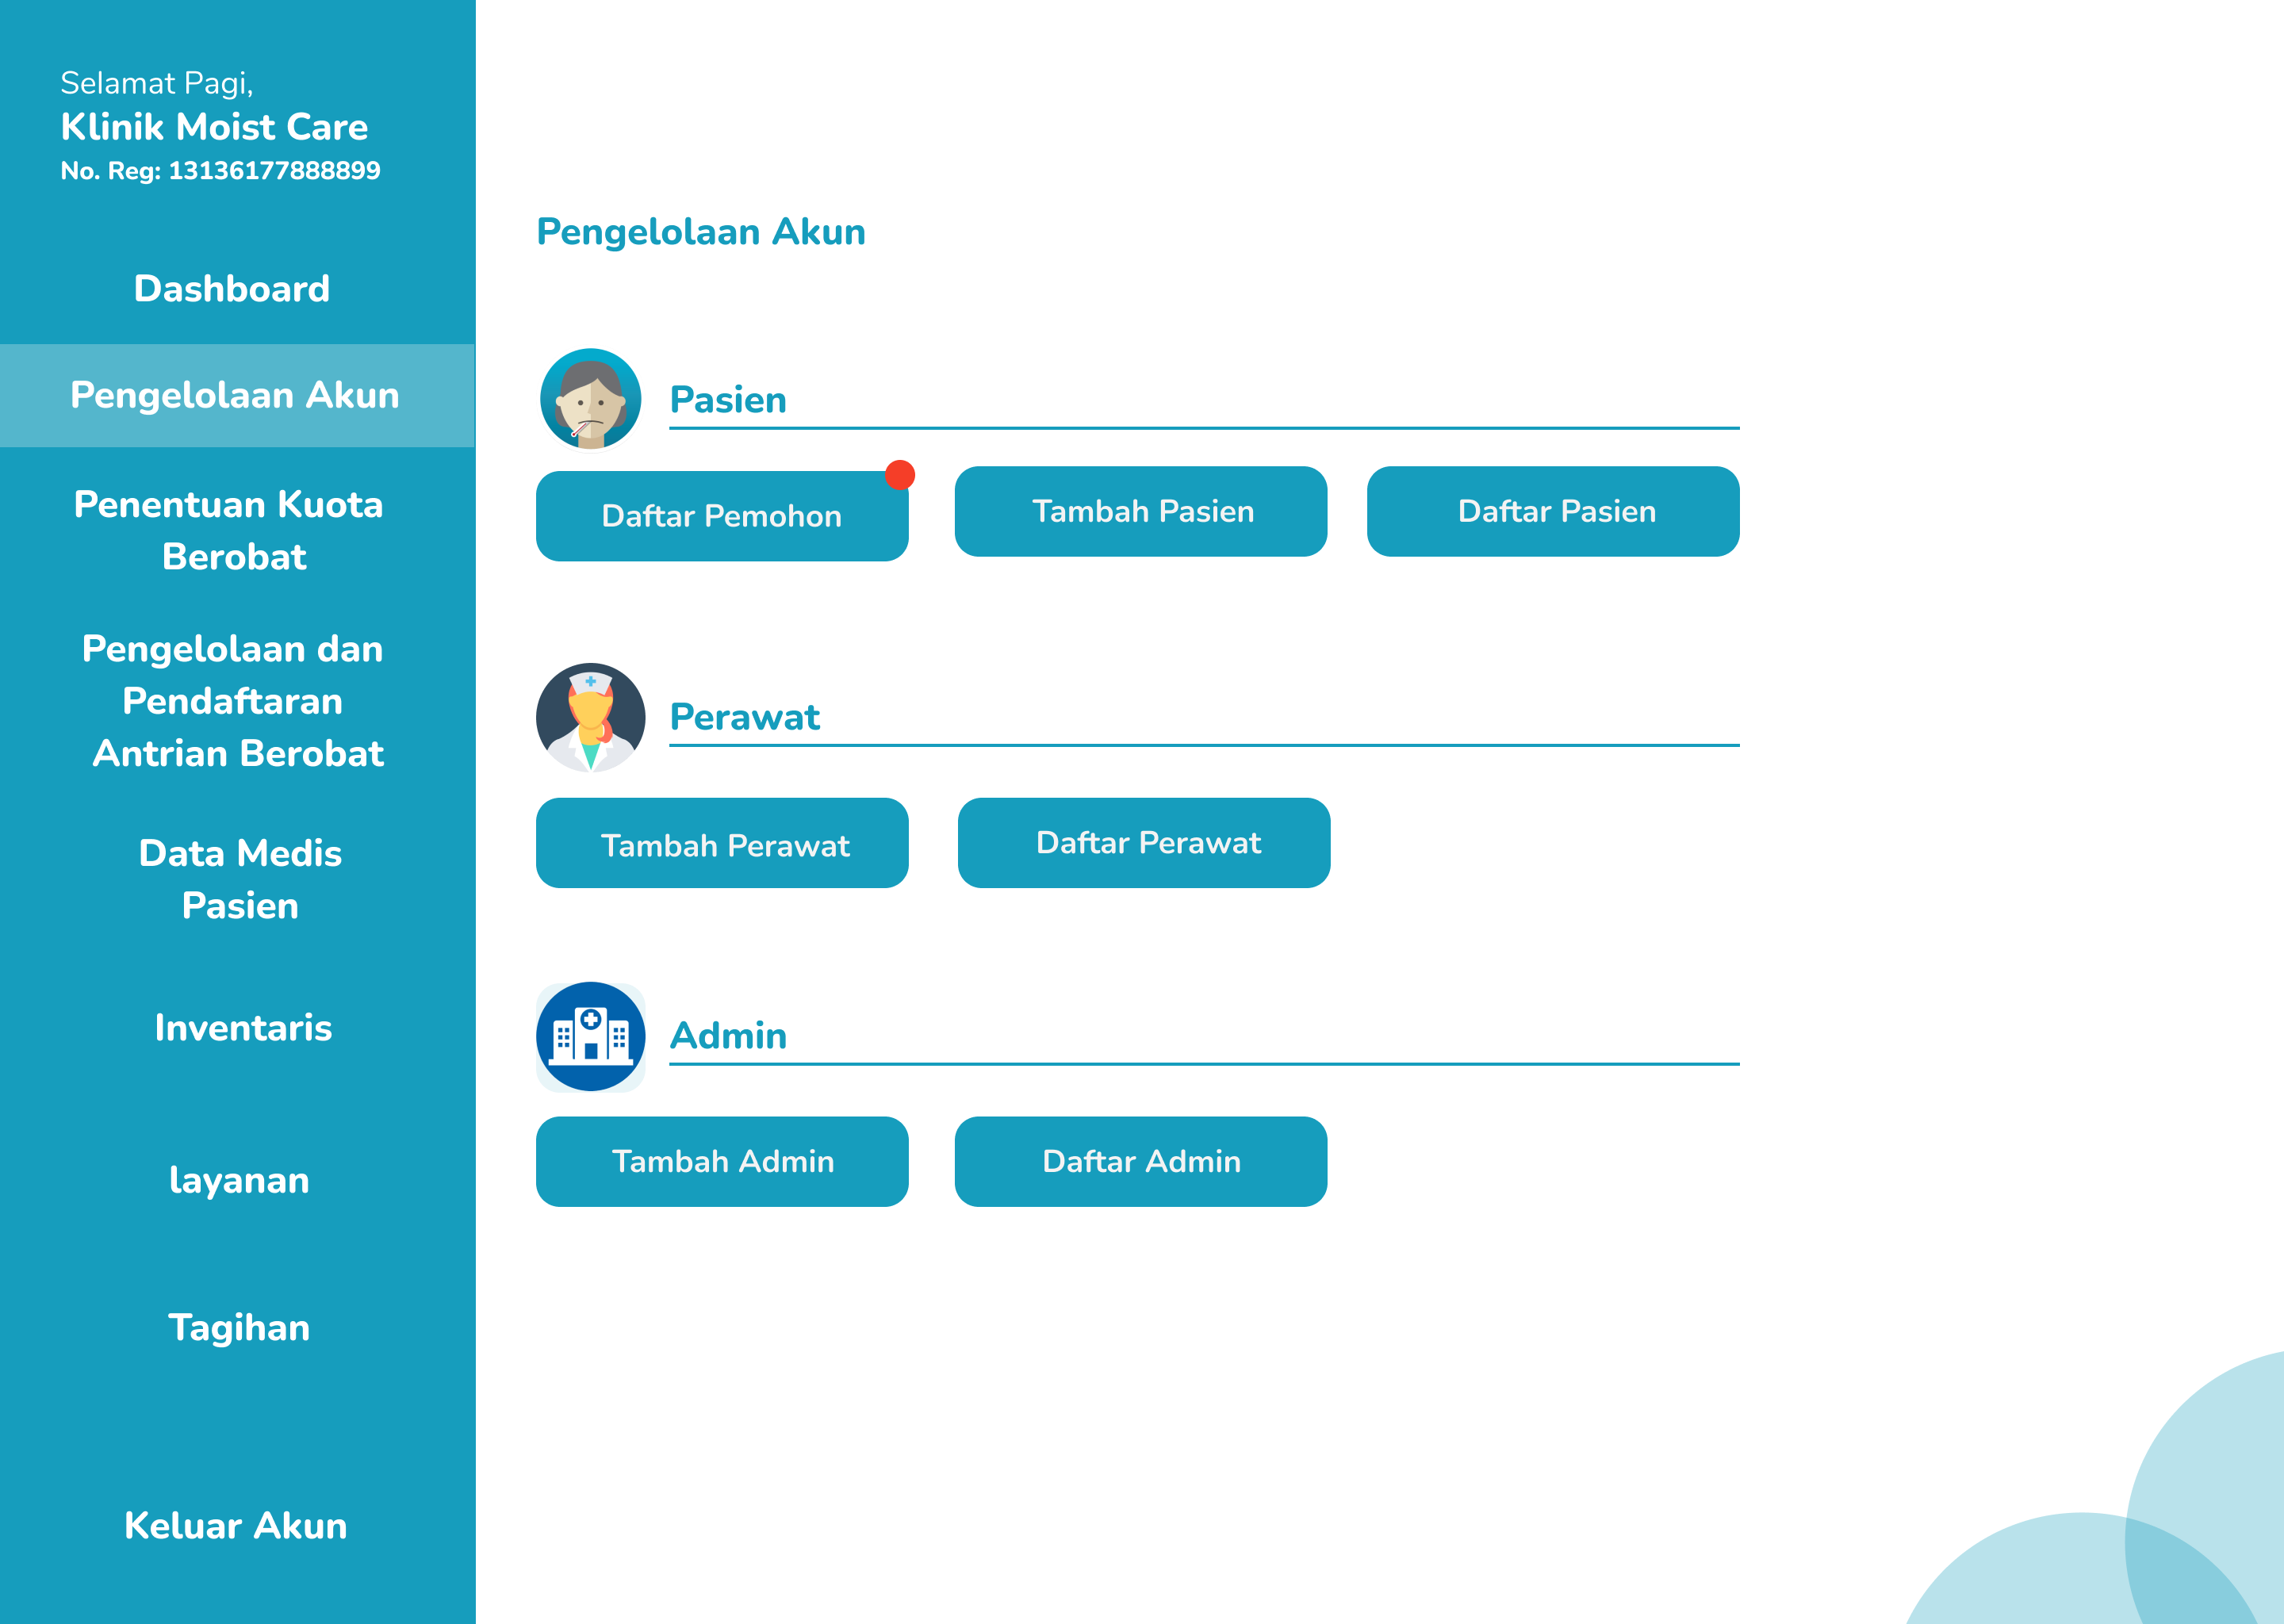
\includegraphics[width=12cm]{gambar/mockup_web/Pembuatan Akun 1.png}
		\caption{\emph{Mock up} tampilan awal pembuatan akun pasien}
		\label{Gambar:tampilanawalpembuatanakunpasien}
	\end{figure}
	
	\textbf{Gambar 4.1} merupakan \emph{mock up} tampilan awal membuat akun pasien. Pada tampilan ini di menu pasien terdapat tombol daftar permohonan pasien untuk melihat \emph{list} akun pasien yang menunggu untuk disetujui pembuatan akunnya. Lalu ada tombol tambah pasien untuk membuat akun pasien baru melalui klinik. Selanjutnya ada tombol daftar pasien untuk melihat semua akun pasien yang terdaftar pada klinik. Di bawah menu pasien ada menu perawat yang berisi tombol tambah perawat untuk membuat akun perawat baru. Lalu tombol daftar perawat untuk melihat semua akun perawat yang terdaftar pada klinik. Selanjutnya di bawah menu perawat ada menu admin yang berisi tombol tambah admin untuk membuat akun admin baru dan ada tombol daftar admin untuk melihat seluruh akun admin yang terdaftar.
	
	Berikutnya saat admin menekan tombol daftar pemohon pada \textbf{Gambar 4.1} maka akan diarahkan ke \textbf{Gambar 4.2}.
	 
	\begin{figure}[H]
		\centering
		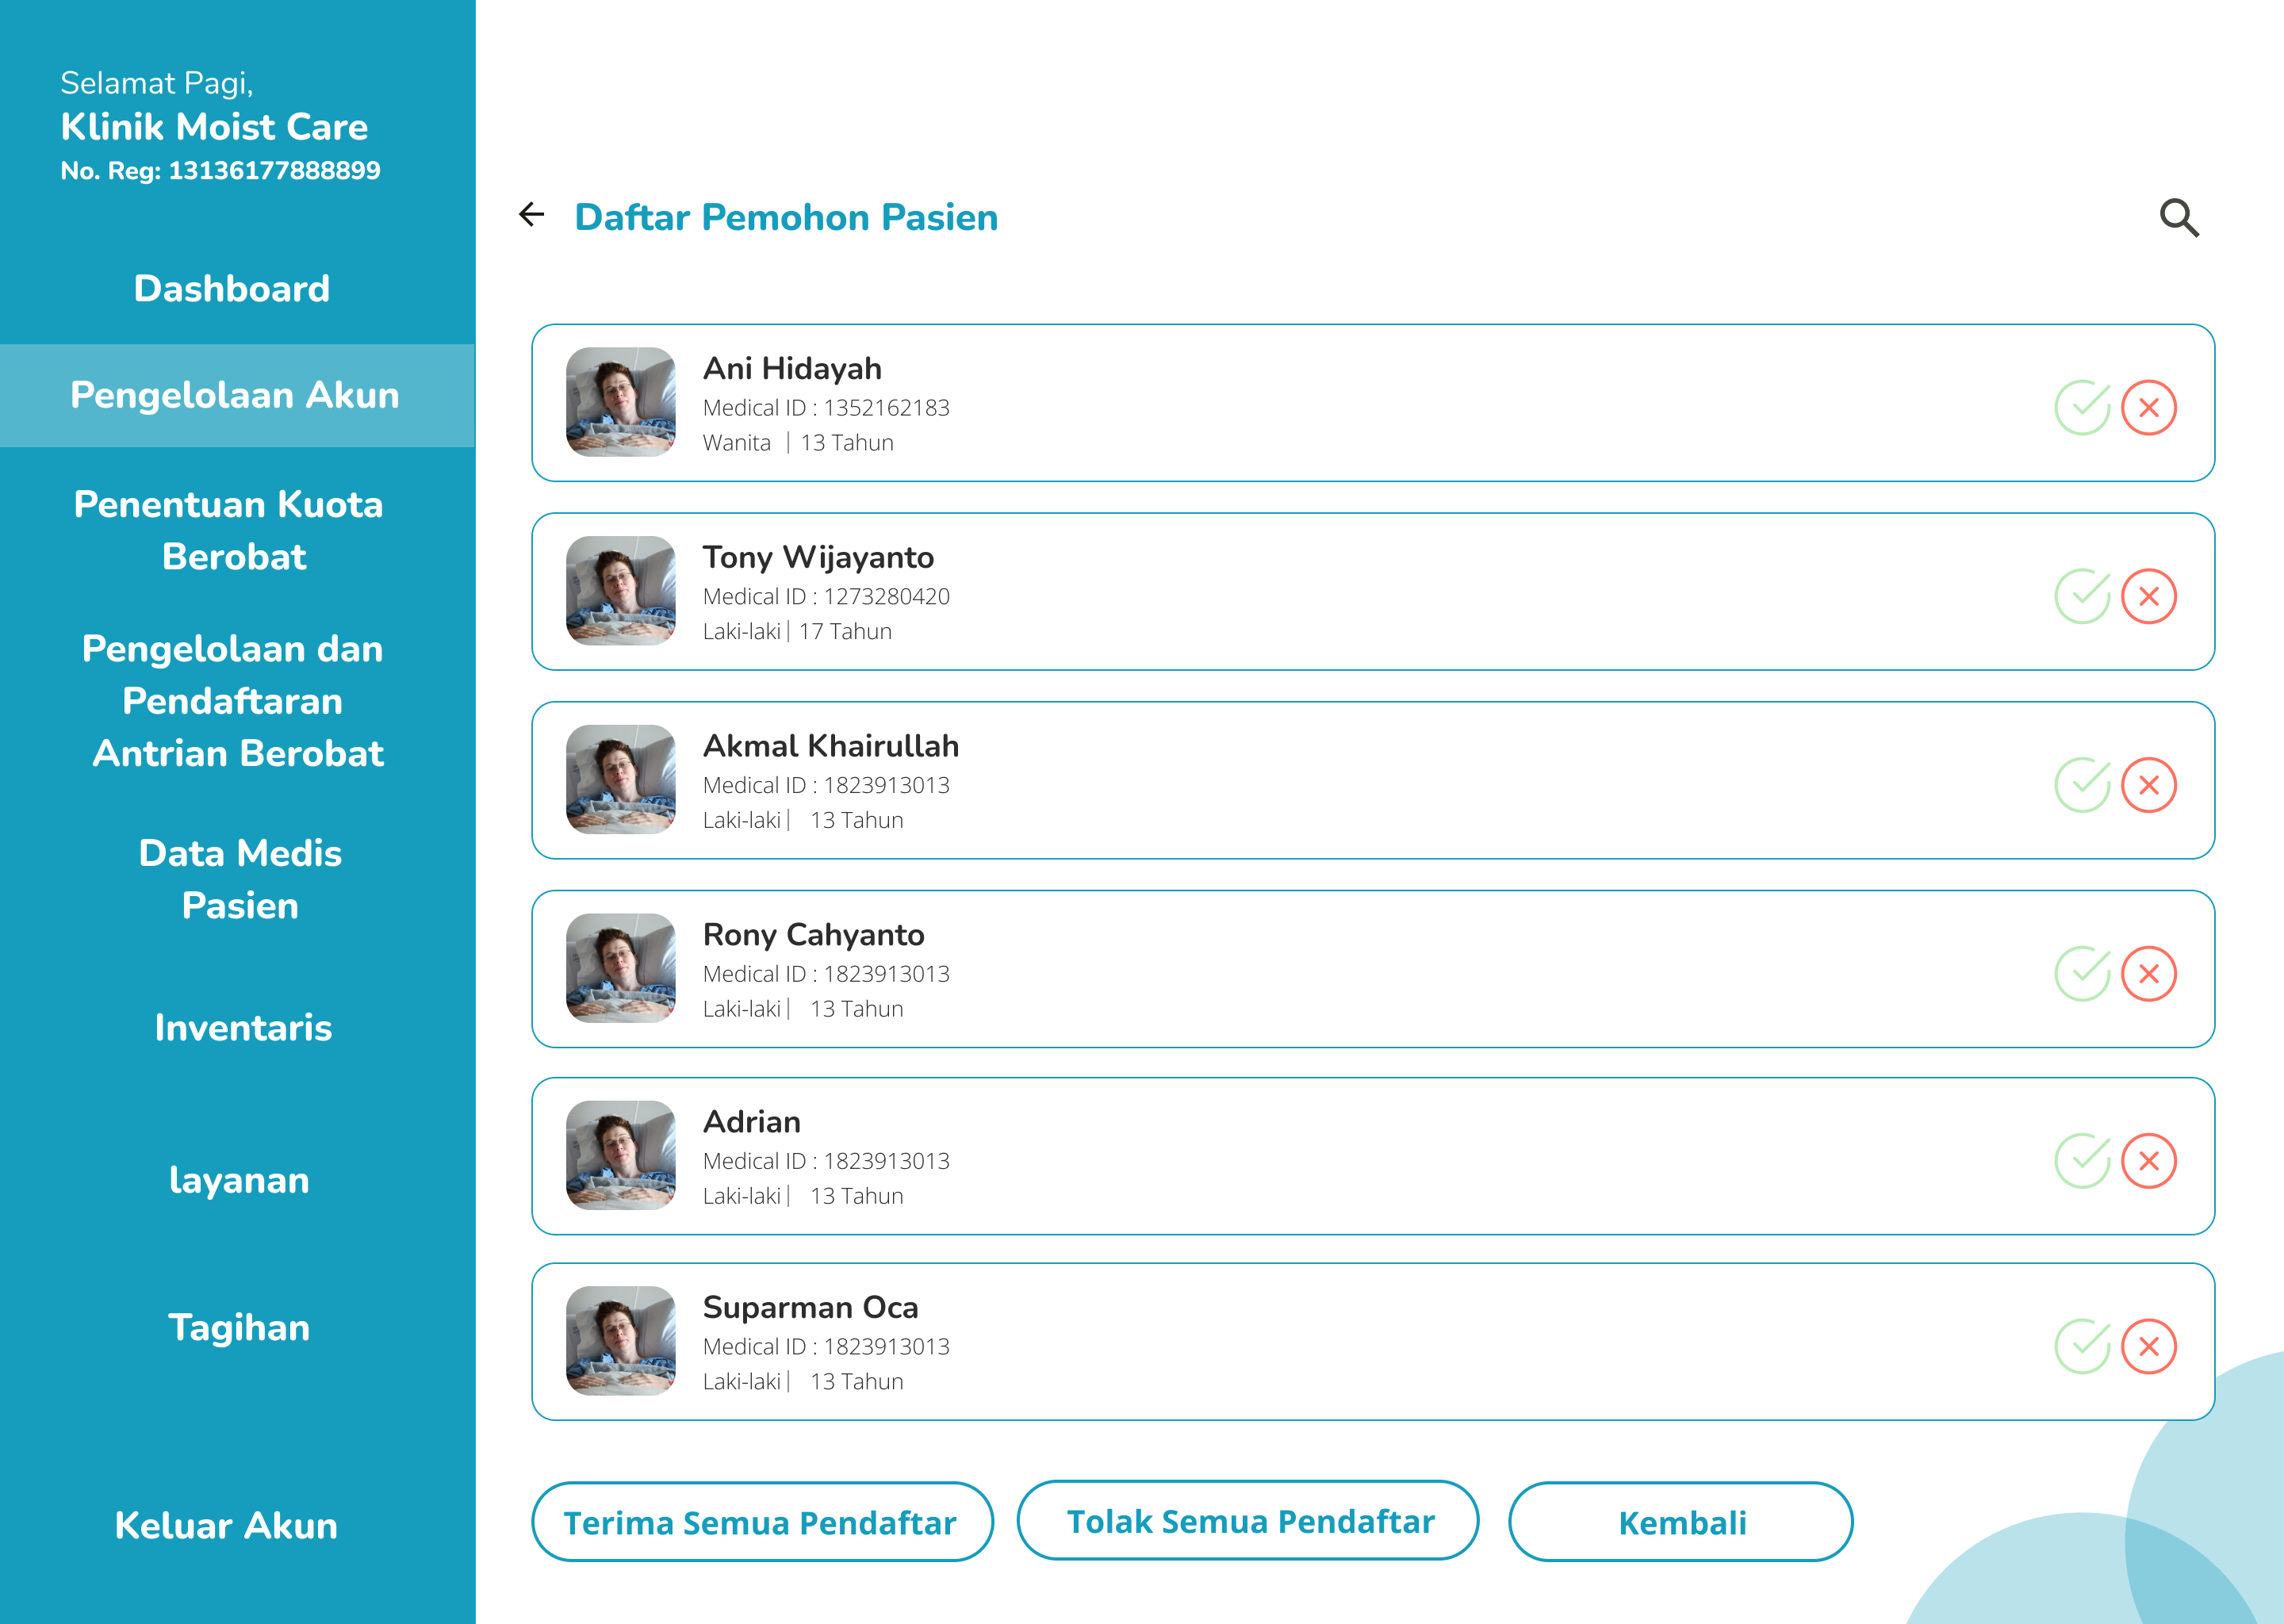
\includegraphics[width=12cm]{gambar/mockup_web/Pembuatan Akun 2.png}
		\caption{\emph{Mock up} tampilan \emph{list} permohonan  pembuatan akun pasien}
		\label{Gambar:listpermohonanpembuatanakunpasien}
	\end{figure}

	\textbf{Gambar 4.2} merupakan tampilan \emph{list} permohonan pembuatan akun pasien. Berisi \emph{list} akun yang menunggu untuk disetujui pembuatan akunnya oleh klinik. Di bawah terdapat tombol terima semua pendaftar untuk menyetujui semua akun yang ada pada \emph{list} permohonan pasien. 	Lalu ada tombol tolak semua pendaftar untuk menolak semua akun yang ada pada \emph{list} permohonan pasien. Dan ada tombol kembali untuk kembali ke tampilan awal pembuatan akun pasien.
	
	Berikutnya ketika admin menekan tombol tambah pasien pada \textbf{Gambar 4.1} maka akan diarahkan ke \textbf{Gambar 4.3}. 
	
	\begin{figure}[H]
		\centering
		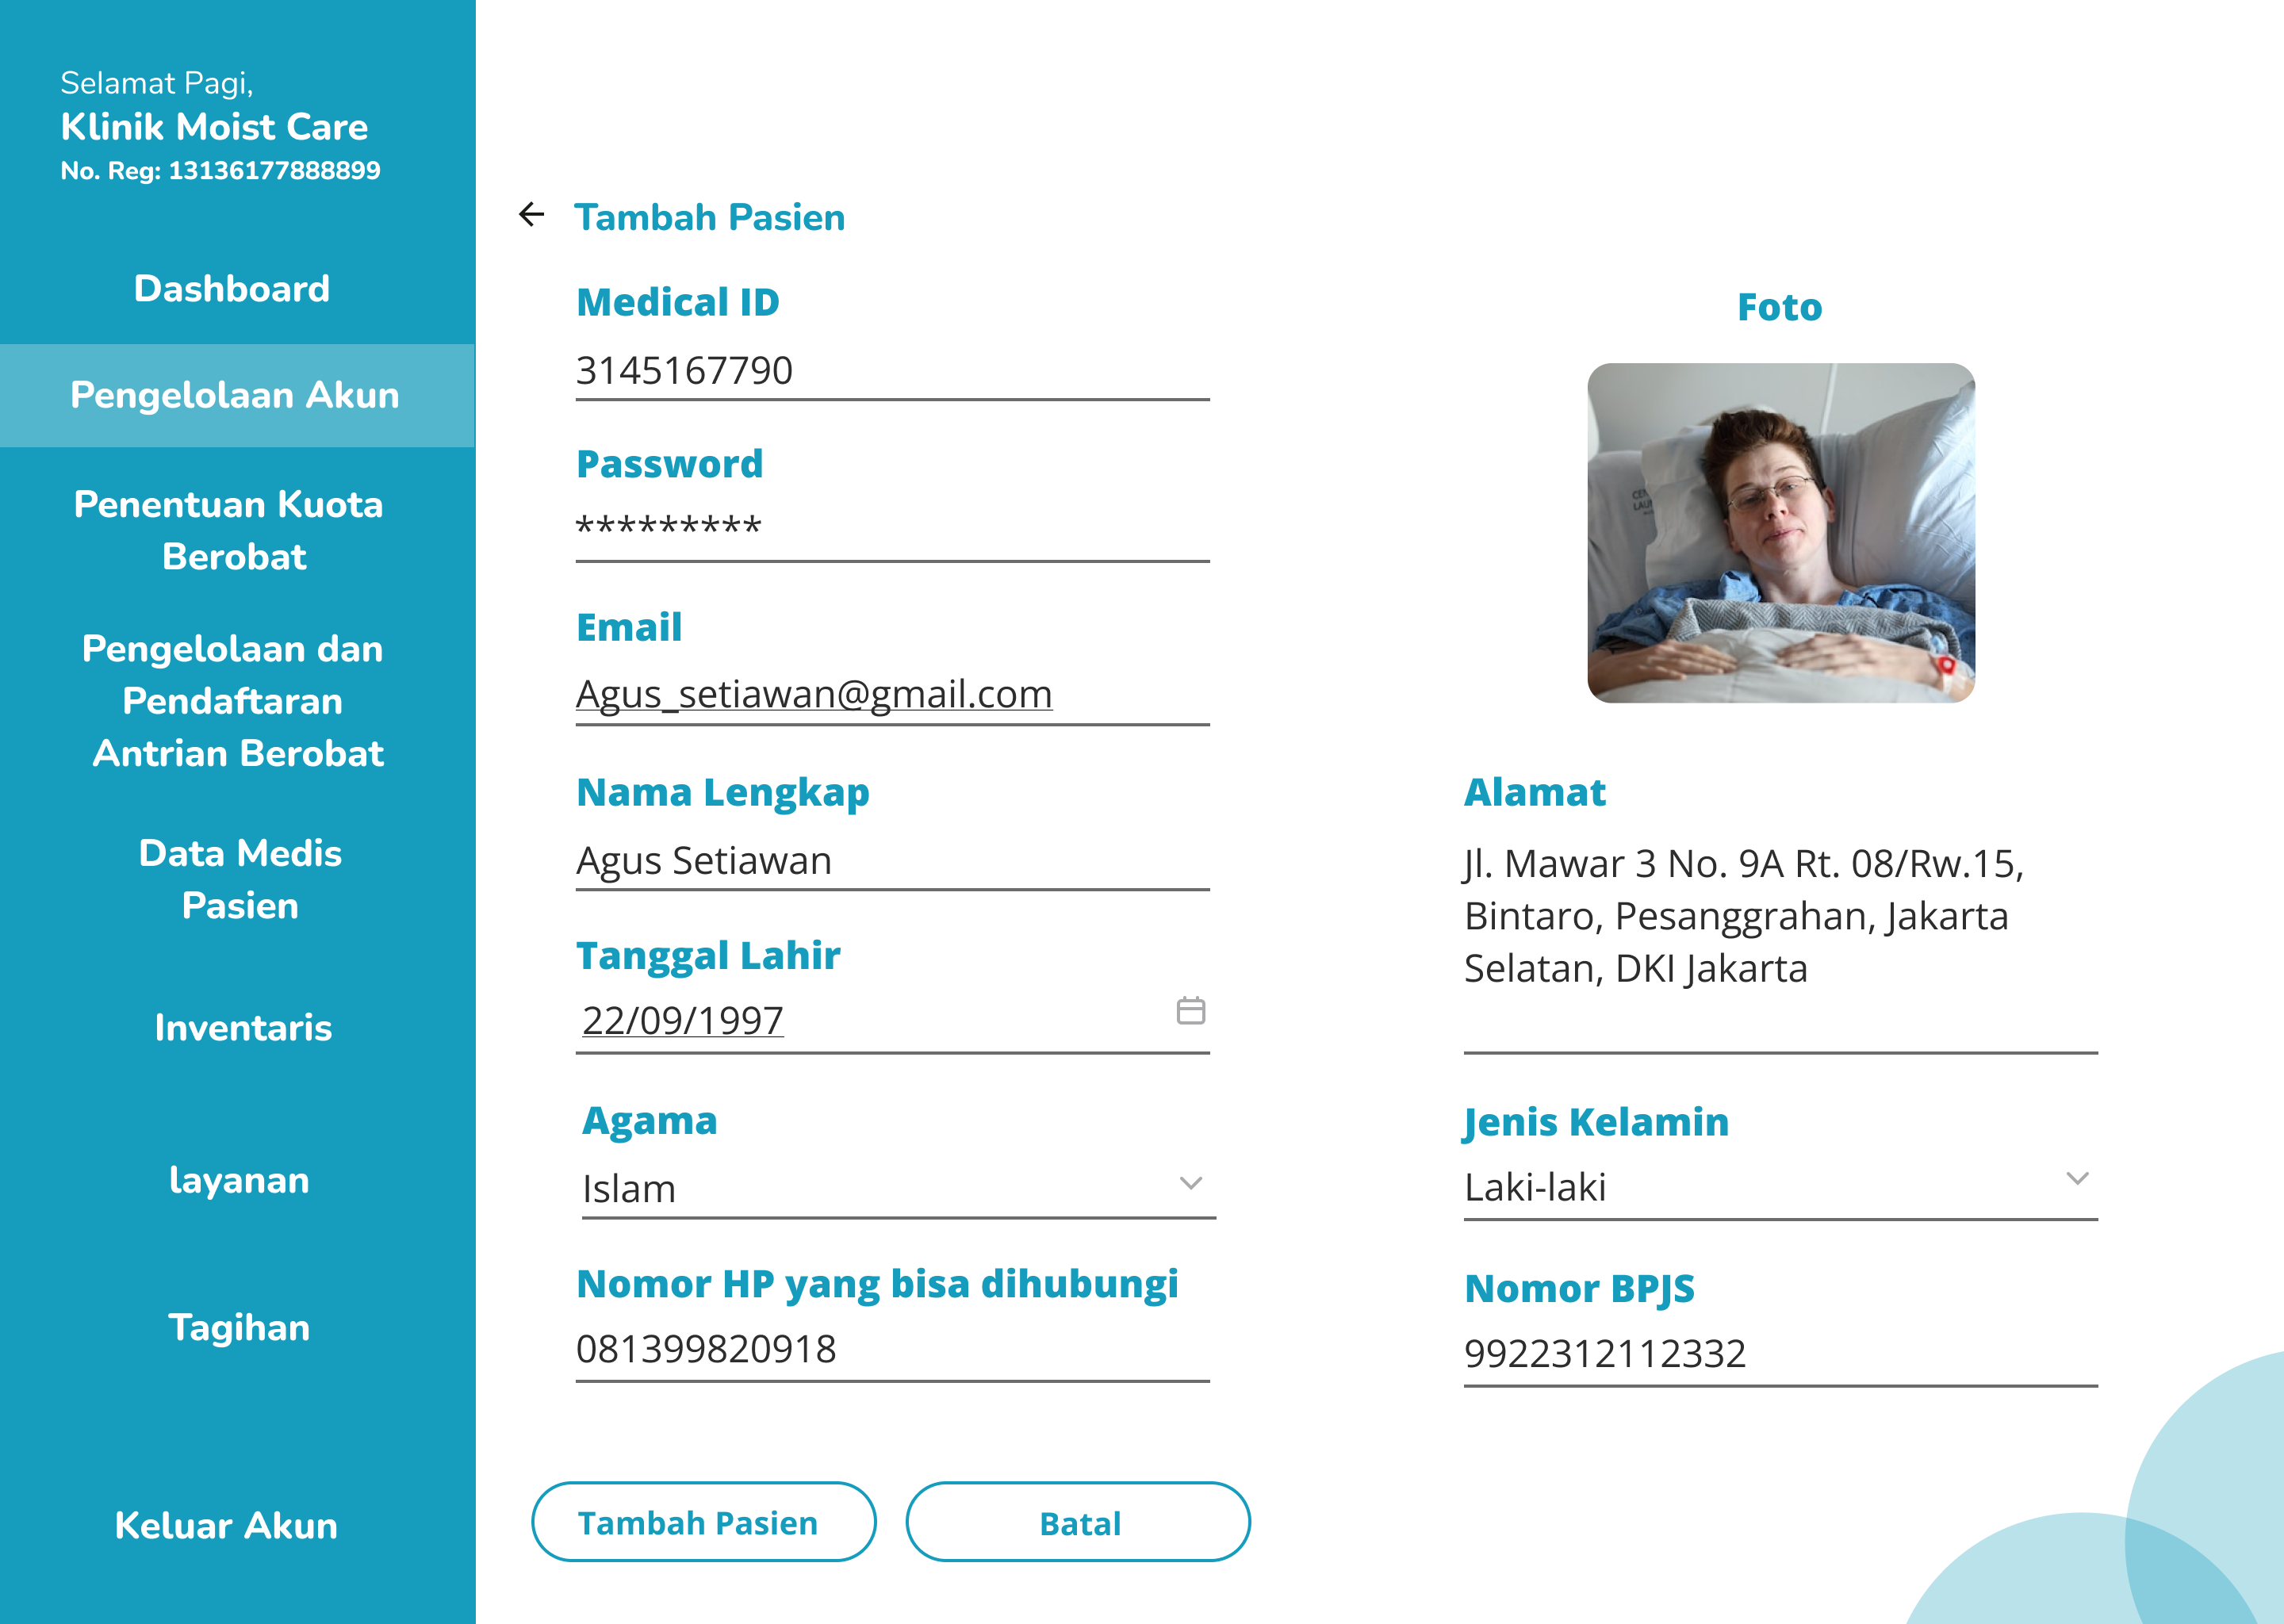
\includegraphics[width=12cm]{gambar/mockup_web/Pembuatan Akun 3.png}
		\caption{\emph{Mock up} pembuatan akun pasien}
		\label{Gambar:pembuatanakunpasien}
	\end{figure}
	
	\textbf{Gambar 4.3} merupakan tampilan pembuatan akun pasien. Saat membuat akun pasien data yang harus diisi adalah medical ID, password, email, nama lengkap, tanggal lahir, agama, Nomor HP yang bisa dihubungi, Nomor BPJS, alamat, foto dan jenis kelamin pasien. Lalu di bawah ada tombol tambah pasien untuk menyimpan akun pasien dan ada tombol batal untuk membatalkan tambah akun pasien yang mengarah kembali ke \textbf{Gambar 4.1}. 
	
	\item Desain \emph{routing table} pembuatan akun pasien
	
	\textbf{Tabel 4.4} pada halaman selanjutnya merupakan \emph{routing table} pembuatan akun pasien:
	
	\begin{table}[H]
		\centering
		\caption{\emph{Routing table} pembuatan akun pasien}
		\label{tabel_input}
		\begin{tabular}{|c|c|c|c|c|c|}
			\hline
			\textbf{\emph{Group}} & \textbf{\emph{Name}} & \textbf{API} & \textbf{HTTP} & \textbf{Keterangan} & \textbf{\emph{Return}} \\
			
			& & \textbf{\emph{Endpoint}} & \textbf{\emph{Verb}} & & \textbf{\emph{Type}} \\
			\hline

			Pasien & 
			\emph{CREATE} &
			\emph{/add\_new\_}
			&
			\emph{POST} &
			menampilkan halaman &
			\emph{view}\\
			
			& 
			&
			\emph{patient}&
			&
			tambah pasien oleh&\\
			
			& 
			&
			&
			&
			klinik&\\
			\hline
			
			& 
			\emph{READ} &
			\emph{/list\_patient}&
			\emph{GET} &
			Menampilkan halaman&
			\emph{view}\\
			
			& 
			&
			&
			&
			seluruh pasien yang &\\
			
			& 
			&
			&
			&
			sudah terverifikasi &\\
			
			& 
			&
			&
			&
			oleh klinik &\\
			\hline
			
			& 
			\emph{READ} &
			\emph{/list\_request}
			&
			\emph{GET} &
			menampilkan halaman &
			\emph{view}\\
			
			& 
			&
			\emph{\_new\_patient}&
			&
			\emph{list} pasien yang &\\
			
			& 
			&
			&
			&
			membuat akun mandiri&\\
			
			
			& 
			&
			&
			&
			dan belum terverifikasi&\\
			
			& 
			&
			&
			&
			oleh klinik&\\
			\hline
			
			Pasien& 
			\emph{READ} &
			\emph{/profil\_pasien}&
			\emph{GET} &
			Menampilkan halaman &
			\emph{view}\\
			
			& 
			&
			\emph{/<\_id>}&
			&
			data pasien&\\
			
			& 
			&
			&
			&
			berdasarkan id pasien&\\
			\hline
			
		\end{tabular}
	\end{table}
	
	\item Membuat \emph{database} pasien
	
	\textbf{Gambar 4.4} pada halaman selanjutnya merupakan tabel pasien yang memuat beberapa atribut yaitu id\_pasien, \emph{password}, id\_staff\_klinik, nama dan agama, tanggal\_lahir, usia, jenis\_kelamin, alamat, no\_hp, email, no\_bpjs, verif, \emph{list\_image\_id}, \emph{created\_at} dan \emph{update\_at} . Data tersebut akan disimpan pada \emph{database} MongoDB dan disimpan dalam format JSON. Tabel atau \emph{collection} pasien akan dibuat bersamaan dengan pemanggilan REST API pembuatan akun pasien.
	
	\begin{figure}[H]
		\centering
		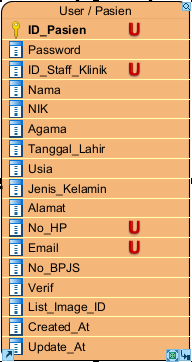
\includegraphics[width=4cm]{gambar/database_pasien.png}
		\caption{Tabel Pasien}
		\label{Gambar:pembuatanakunpasien}
	\end{figure}
	
	\item Pembuatan \emph{mock up} \emph{dashboard} klinik
	
	\begin{figure}[H]
		\centering
		\includegraphics[width=12cm]{gambar/mockup_web/dashboard.png}
		\caption{\emph{Mock up} tampilan awal dashboard klinik}
		\label{Gambar:pengelolaanantrian2}
	\end{figure}
	
	\textbf{Gambar 4.5} merupakan tampilan \emph{dashboard} klinik. Admin dapat melihat statistik kinerja perawat, \emph{cost} perawatan pasien, \emph{income} masuk dan \emph{balance} keuangan dengan detail rata-rata harian, mingguan, dan bulanan.
	
	\item Desain \emph{routing table dashboard} klinik
	
	\textbf{Tabel 4.5} merupakan \emph{routing table} untuk \emph{dashboard} klinik:
	
	\begin{table}[H]
		\centering
		\caption{\emph{Routing table dashboard} klinik}
		\label{tabel_input}
		\begin{tabular}{|c|c|c|c|c|c|}
			\hline
			\textbf{\emph{Group}} & \textbf{\emph{Name}} & \textbf{API} & \textbf{HTTP} & \textbf{Keterangan} & \textbf{\emph{Return}} \\
			
			& & \textbf{\emph{Endpoint}} & \textbf{\emph{Verb}} & & \textbf{\emph{Type}} \\
			\hline
			
			\emph{Dashboard}& 
			\emph{READ} &
			/ &
			\emph{GET} &
			Menampilkan halaman &
			\emph{view}\\
			
			& 
			&
			&
			&
			\emph{dashboard} klinik &
			\\
			\hline
			
		\end{tabular}
	\end{table}
	
	\item Desain \emph{routing table} pemeriksaan kesehatan
	
	\textbf{Tabel 4.6} dan \textbf{Tabel 4.7} merupakan \emph{routing table} untuk pemeriksaan kesehatan:
	
	\begin{table}[H]
		\centering
		\caption{\emph{Routing table} pemeriksaan kesehatan}
		\label{tabel_input}
		\begin{tabular}{|c|c|c|c|c|c|}
			\hline
			\textbf{\emph{Group}} & \textbf{\emph{Name}} & \textbf{API} & \textbf{HTTP} & \textbf{Keterangan} & \textbf{\emph{Return}} \\
			
			& & \textbf{\emph{Endpoint}} & \textbf{\emph{Verb}} & & \textbf{\emph{Type}} \\
			\hline
			
			Pemeri-& 
			\emph{READ} &
			/\emph{list\_patient} &
			\emph{GET} &
			Menampilkan halaman &
			\emph{view}\\
			
			ksaan& 
			&
			\_\emph{medical}&
			&
			\emph{list} pasien yang  &
			\\
			
			Keseha-& 
			&
			\_\emph{check}&
			&
			telah melakukan &
			\\
			
			tan& 
			&
			&
			&
			pemeriksaan kesehatan &
			\\
			\hline
			
			& 
			\emph{READ} &
			/\emph{list\_medical} &
			\emph{GET} &
			Menampilkan halaman &
			\emph{view}\\
			
			& 
			&
			\_\emph{\_check\_}&
			&
			\emph{list} hasil pemeriksaan &
			\\
			
			& 
			&
			\_\emph{data/<nik>}&
			&
			kesehatan 1 pasien &
			\\
			\hline				
			
		\end{tabular}
	\end{table}
	
	\begin{table}[H]
		\centering
		\caption{\emph{Routing table} pemeriksaan kesehatan - lanjutan}
		\label{tabel_input}
		\begin{tabular}{|c|c|c|c|c|c|}
			\hline
			\textbf{\emph{Group}} & \textbf{\emph{Name}} & \textbf{API} & \textbf{HTTP} & \textbf{Keterangan} & \textbf{\emph{Return}} \\
			
			& & \textbf{\emph{Endpoint}} & \textbf{\emph{Verb}} & & \textbf{\emph{Type}} \\
			\hline
			
			Pemeri-& 
			\emph{READ} &
			/detail\_ &
			\emph{GET} &
			Menampilkan halaman &
			\emph{view}\\
			
			ksaan& 
			&
			\_\emph{medical\_}&
			&
			detail hasil pemeriksaan &
			\\
			
			Keseha-& 
			&
			check\_data&
			&
			kesehatan &
			\\
			
			tan& 
			&
			/<\_id>&
			&
			&
			\\
			\hline				
			
		\end{tabular}
	\end{table}
	
	\item Membuat \emph{database} pemeriksaan kesehatan
	
	\begin{figure}[H]
		\centering
		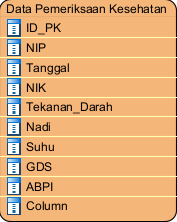
\includegraphics[width=5cm]{gambar/database_data_pemeriksaan_kesehatan.png}
		\caption{Tabel pemeriksaan kesehatan}
		\label{Gambar:pengelolaanantrian2}
	\end{figure}

	\textbf{Gambar 4.6} merupakan tabel pemeriksaan kesehatan memuat beberapa atribut yaitu id\_pk, NIP, tanggal, NIK pasien, tekanan\_darah, nadi, jenis\_kelamin, alamat, no\_hp, email, no\_bpjs, verif, suhu, GDS dan ABPI . Data tersebut akan disimpan pada \emph{database} MongoDB dan disimpan dalam format JSON.
	
	\break
	\item Pembuatan \emph{mock up} proses pengobatan luka
	
	Pada \textbf{Gambar 4.7} pada halaman selanjutnya merupakan tampilan awal data medis pasien. Terdapat \emph{list} data medis pasien beserta tombol lihat. Admin maupun perawat dapat menyeleksi data berdasarkan pasien atau perawat pada \emph{field} dikategorikan berdasarkan perawat. Dan terdapat juga \emph{search bar} untuk mencari data medis pasien berdasarkan kata kunci \emph{Medical} ID atau nomor BPJS.
	
	\begin{figure}[H]
		\centering
		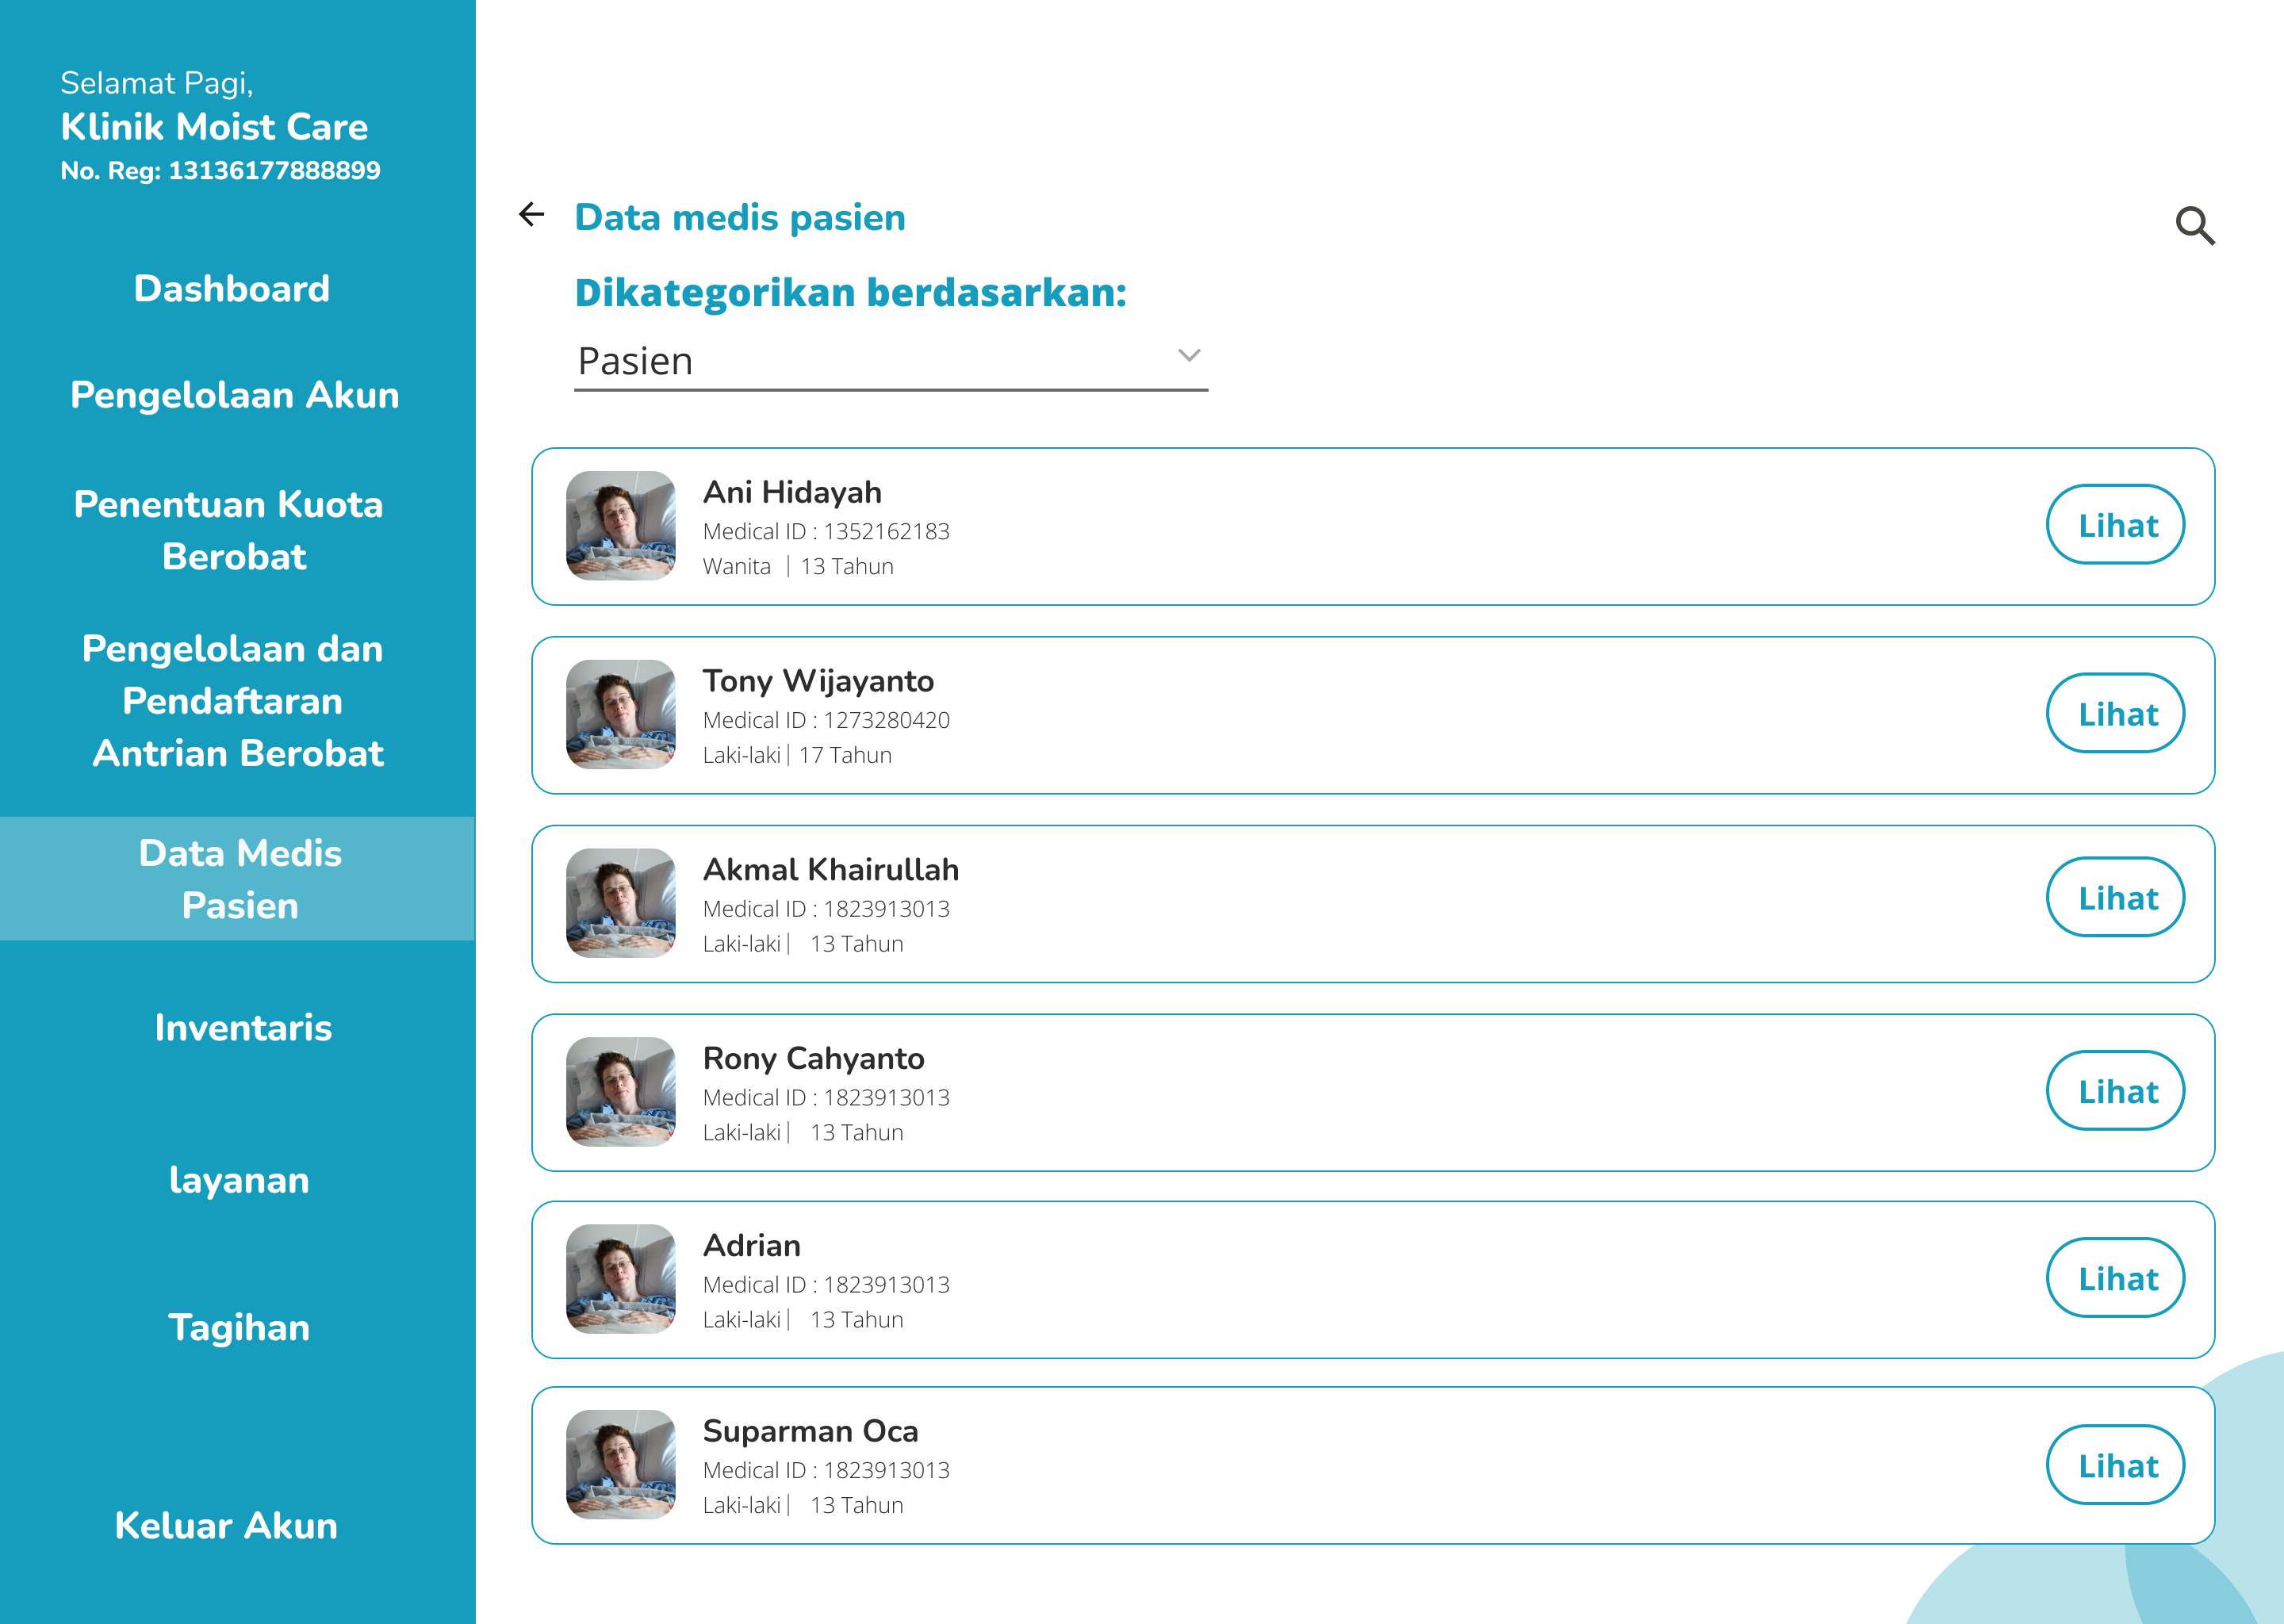
\includegraphics[width=12cm]{gambar/mockup_web/Proses Pengobatan 1.png}
		\caption{\emph{Mock up} tampilan awal data medis pasien}
		\label{Gambar:pengelolaanantrian2}
	\end{figure}
	
	Ketika admin menekan tombol lihat pada data pasien yang dipilih pada \textbf{Gambar 4.7} maka akan diarahkan ke \textbf{Gambar 4.8} pada halaman selanjutnya yang merupakan profil data medis pasien dan berisikan data berupa \emph{Medical} ID, email, nama lengkap, tanggal lahir, agama, nomor hp, alamat, jenis kelamin, foto, dan nomor BPJS. Selanjutnya terdapat tombol profil, histori kajian dan galeri luka. Dan terdapat tombol kembali untuk menuju ke halaman sebelumnya.
	
	\begin{figure}[H]
		\centering
		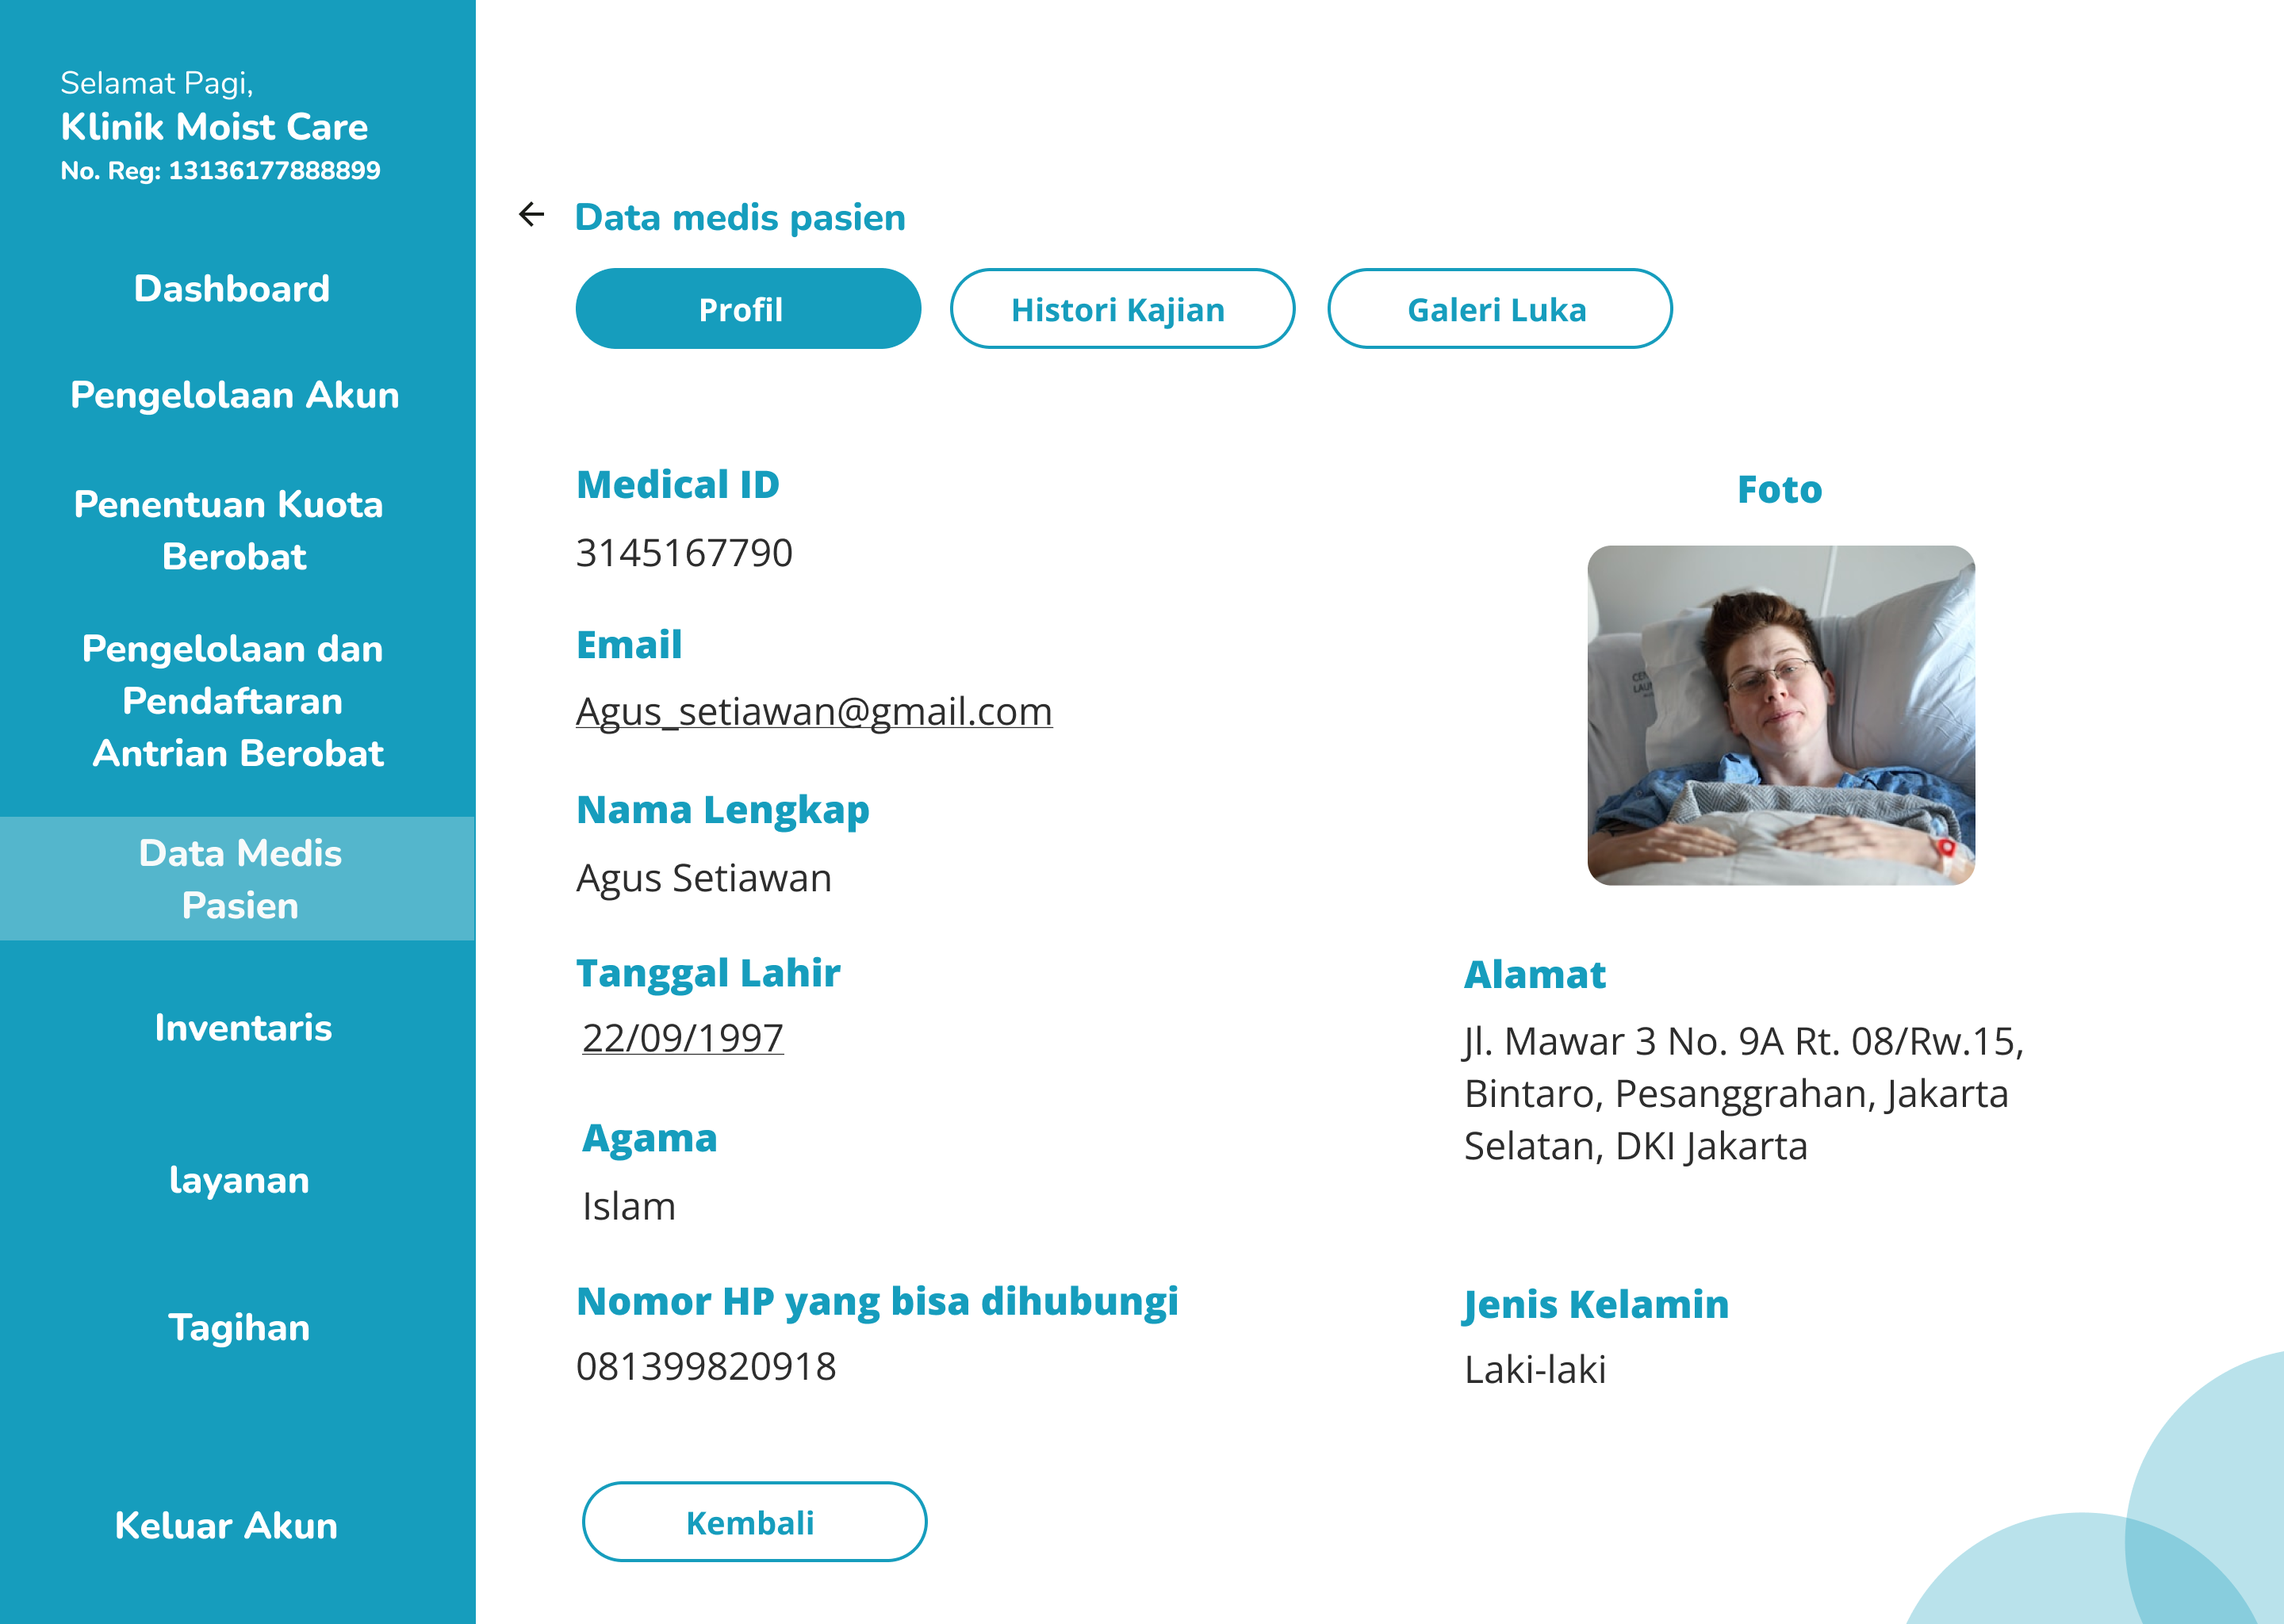
\includegraphics[width=12cm]{gambar/mockup_web/Proses Pengobatan 2.png}
		\caption{\emph{Mock up} profil data medis pasien}
		\label{Gambar:pengelolaanantrian2}
	\end{figure}
	
	Ketika admin menekan tombol histori kajian pada \textbf{Gambar 4.8} maka akan diarahkan ke \textbf{Gambar 4.9}. 
	
	\begin{figure}[H]
		\centering
		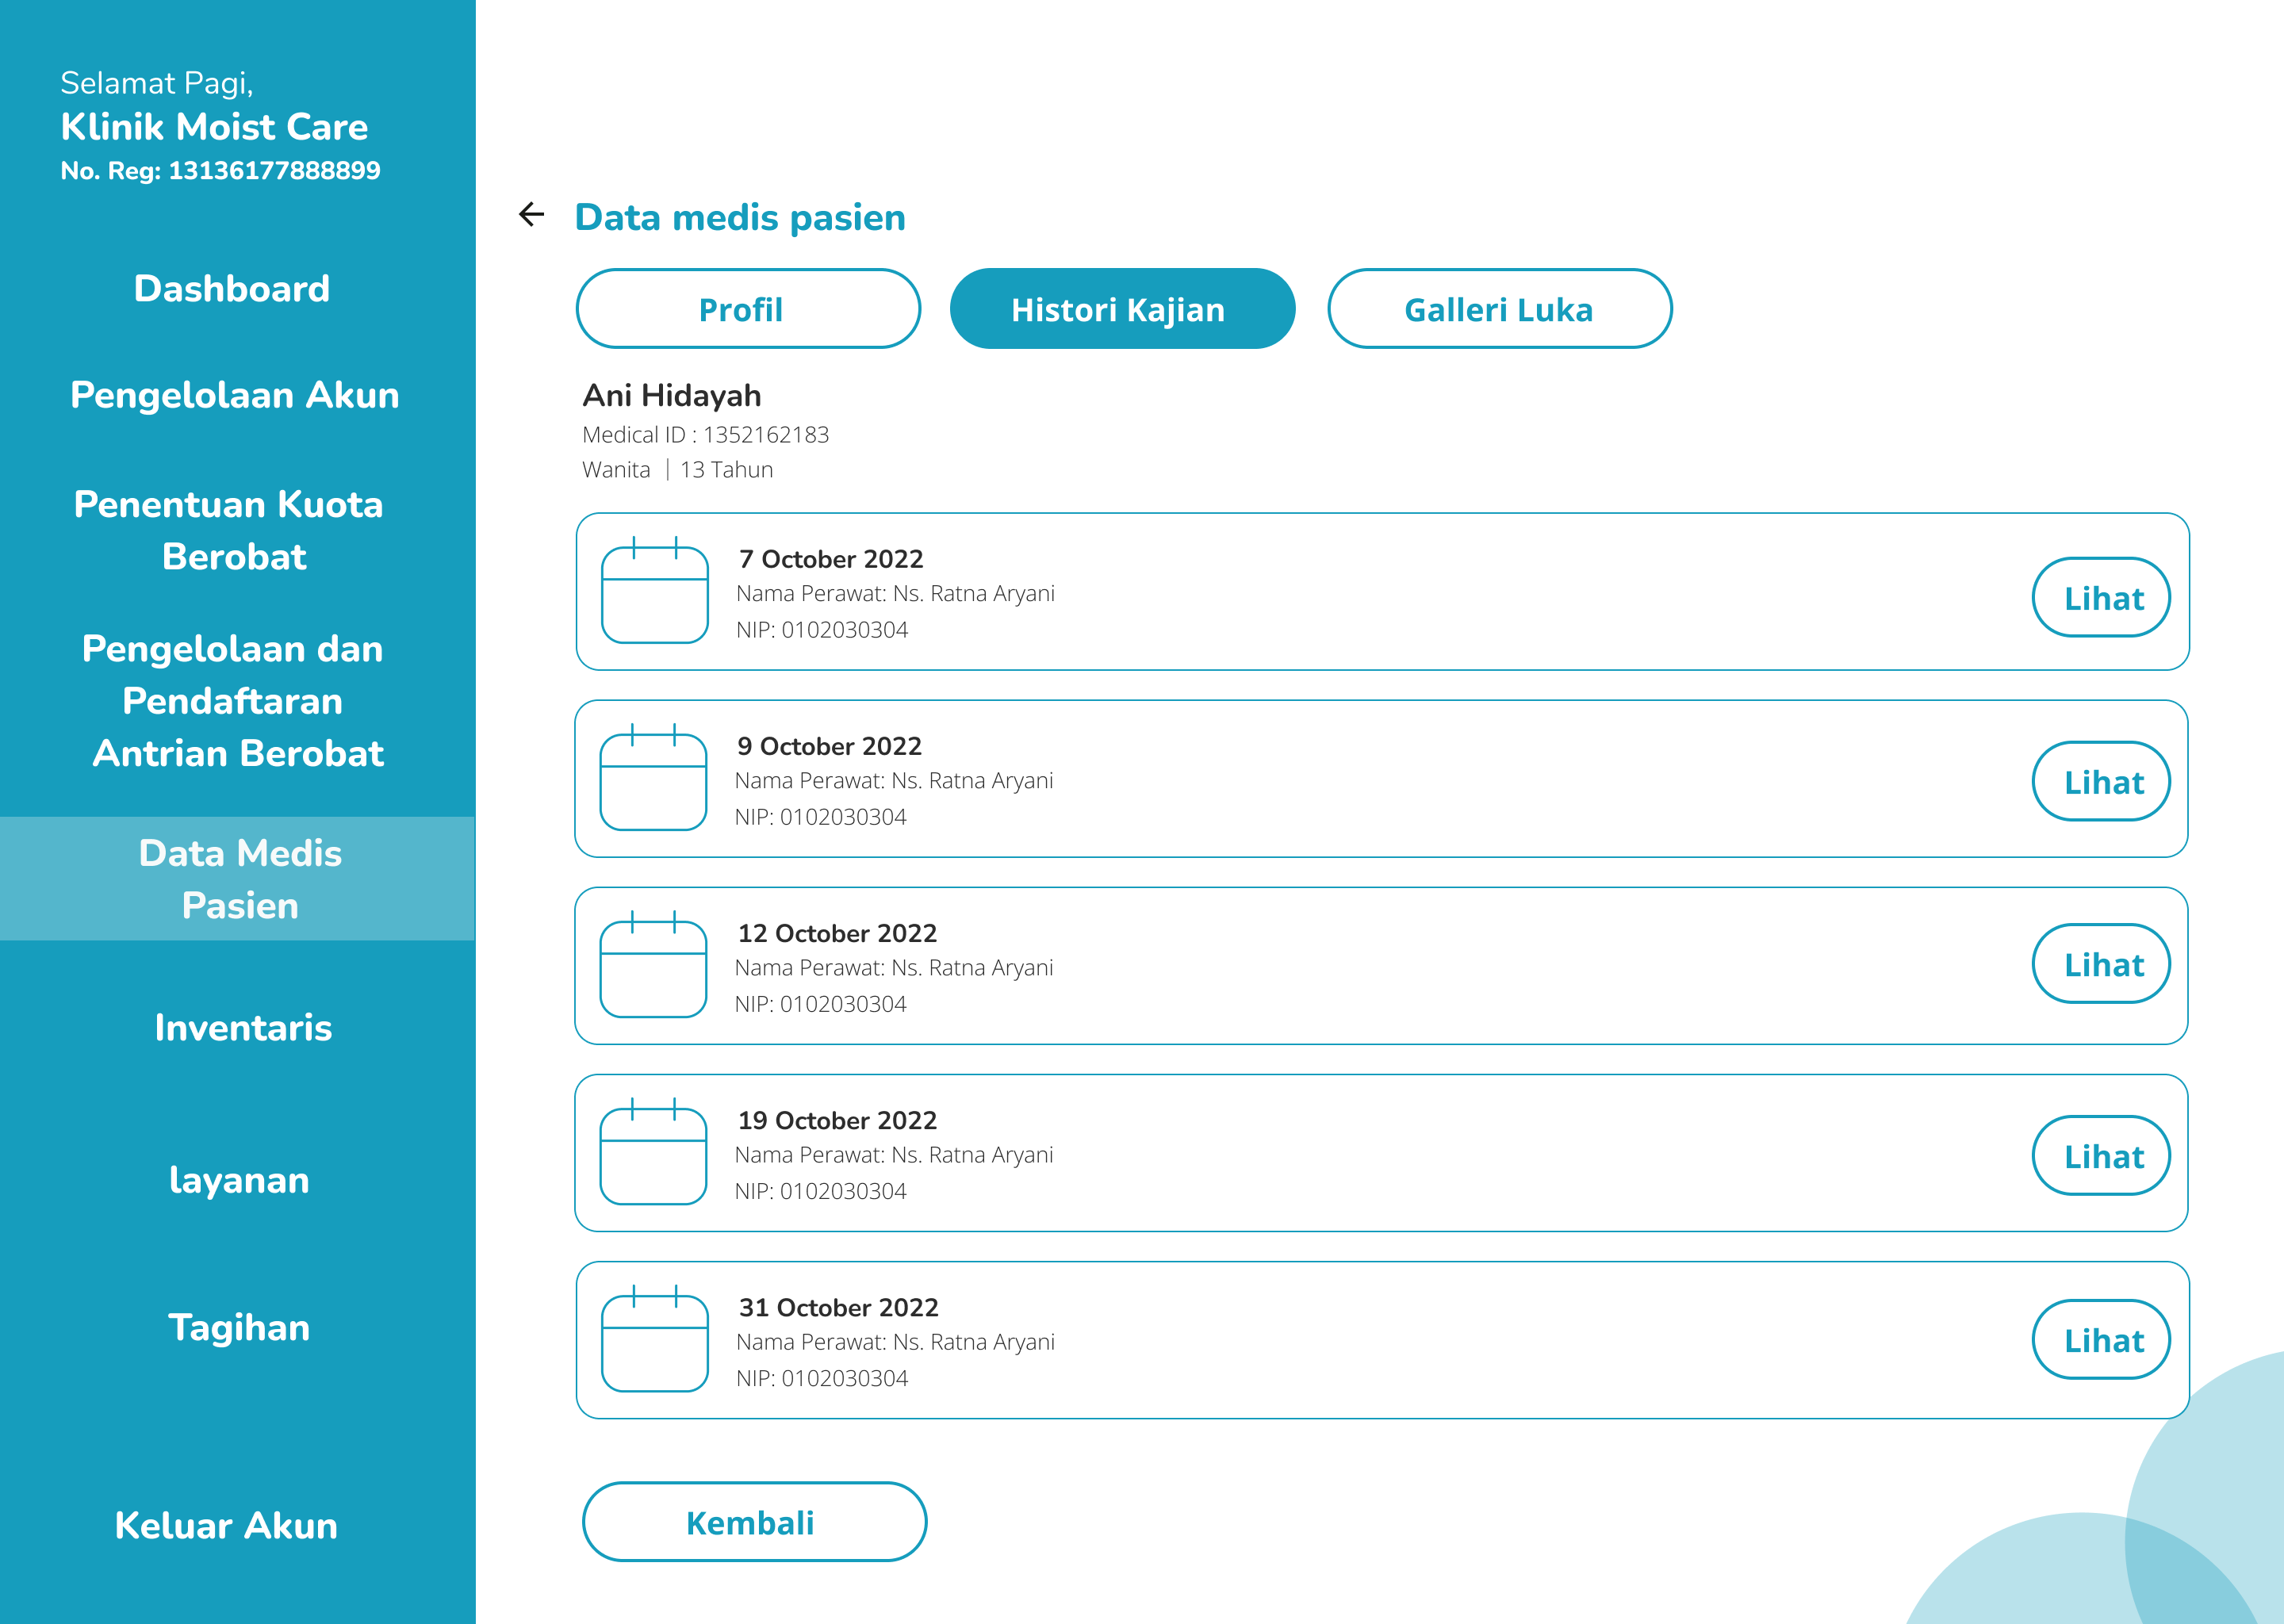
\includegraphics[width=12cm]{gambar/mockup_web/Proses Pengobatan 3.png}
		\caption{\emph{Mock up list} histori kajian data medis pasien}
		\label{Gambar:pengelolaanantrian2}
	\end{figure}
	
	\textbf{Gambar 4.9} merupakan histori kajian data medis pasien berisi \emph{list} kajian yang telah dilaksanakan dan diurutkan berdasarkan tanggal dengan detail data nama dan nip perawat yang melakukan kajian beserta tombol lihat. Dan terdapat tombol kembali untuk menuju ke halaman sebelumnya.
	
	Ketika admin menekan tombol lihat pada salah satu histori kajian pada \textbf{Gambar 4.9} maka akan diarahkan ke \textbf{Gambar 4.10} yang merupakan detail histori kajian data medis pasien berisi foto luka yang diambil saat kajian berlangsung dan skoring kajian luka pasien. Dan terdapat tombol kembali untuk kembali ke halaman sebelumnya.
	
	\begin{figure}[H]
		\centering
		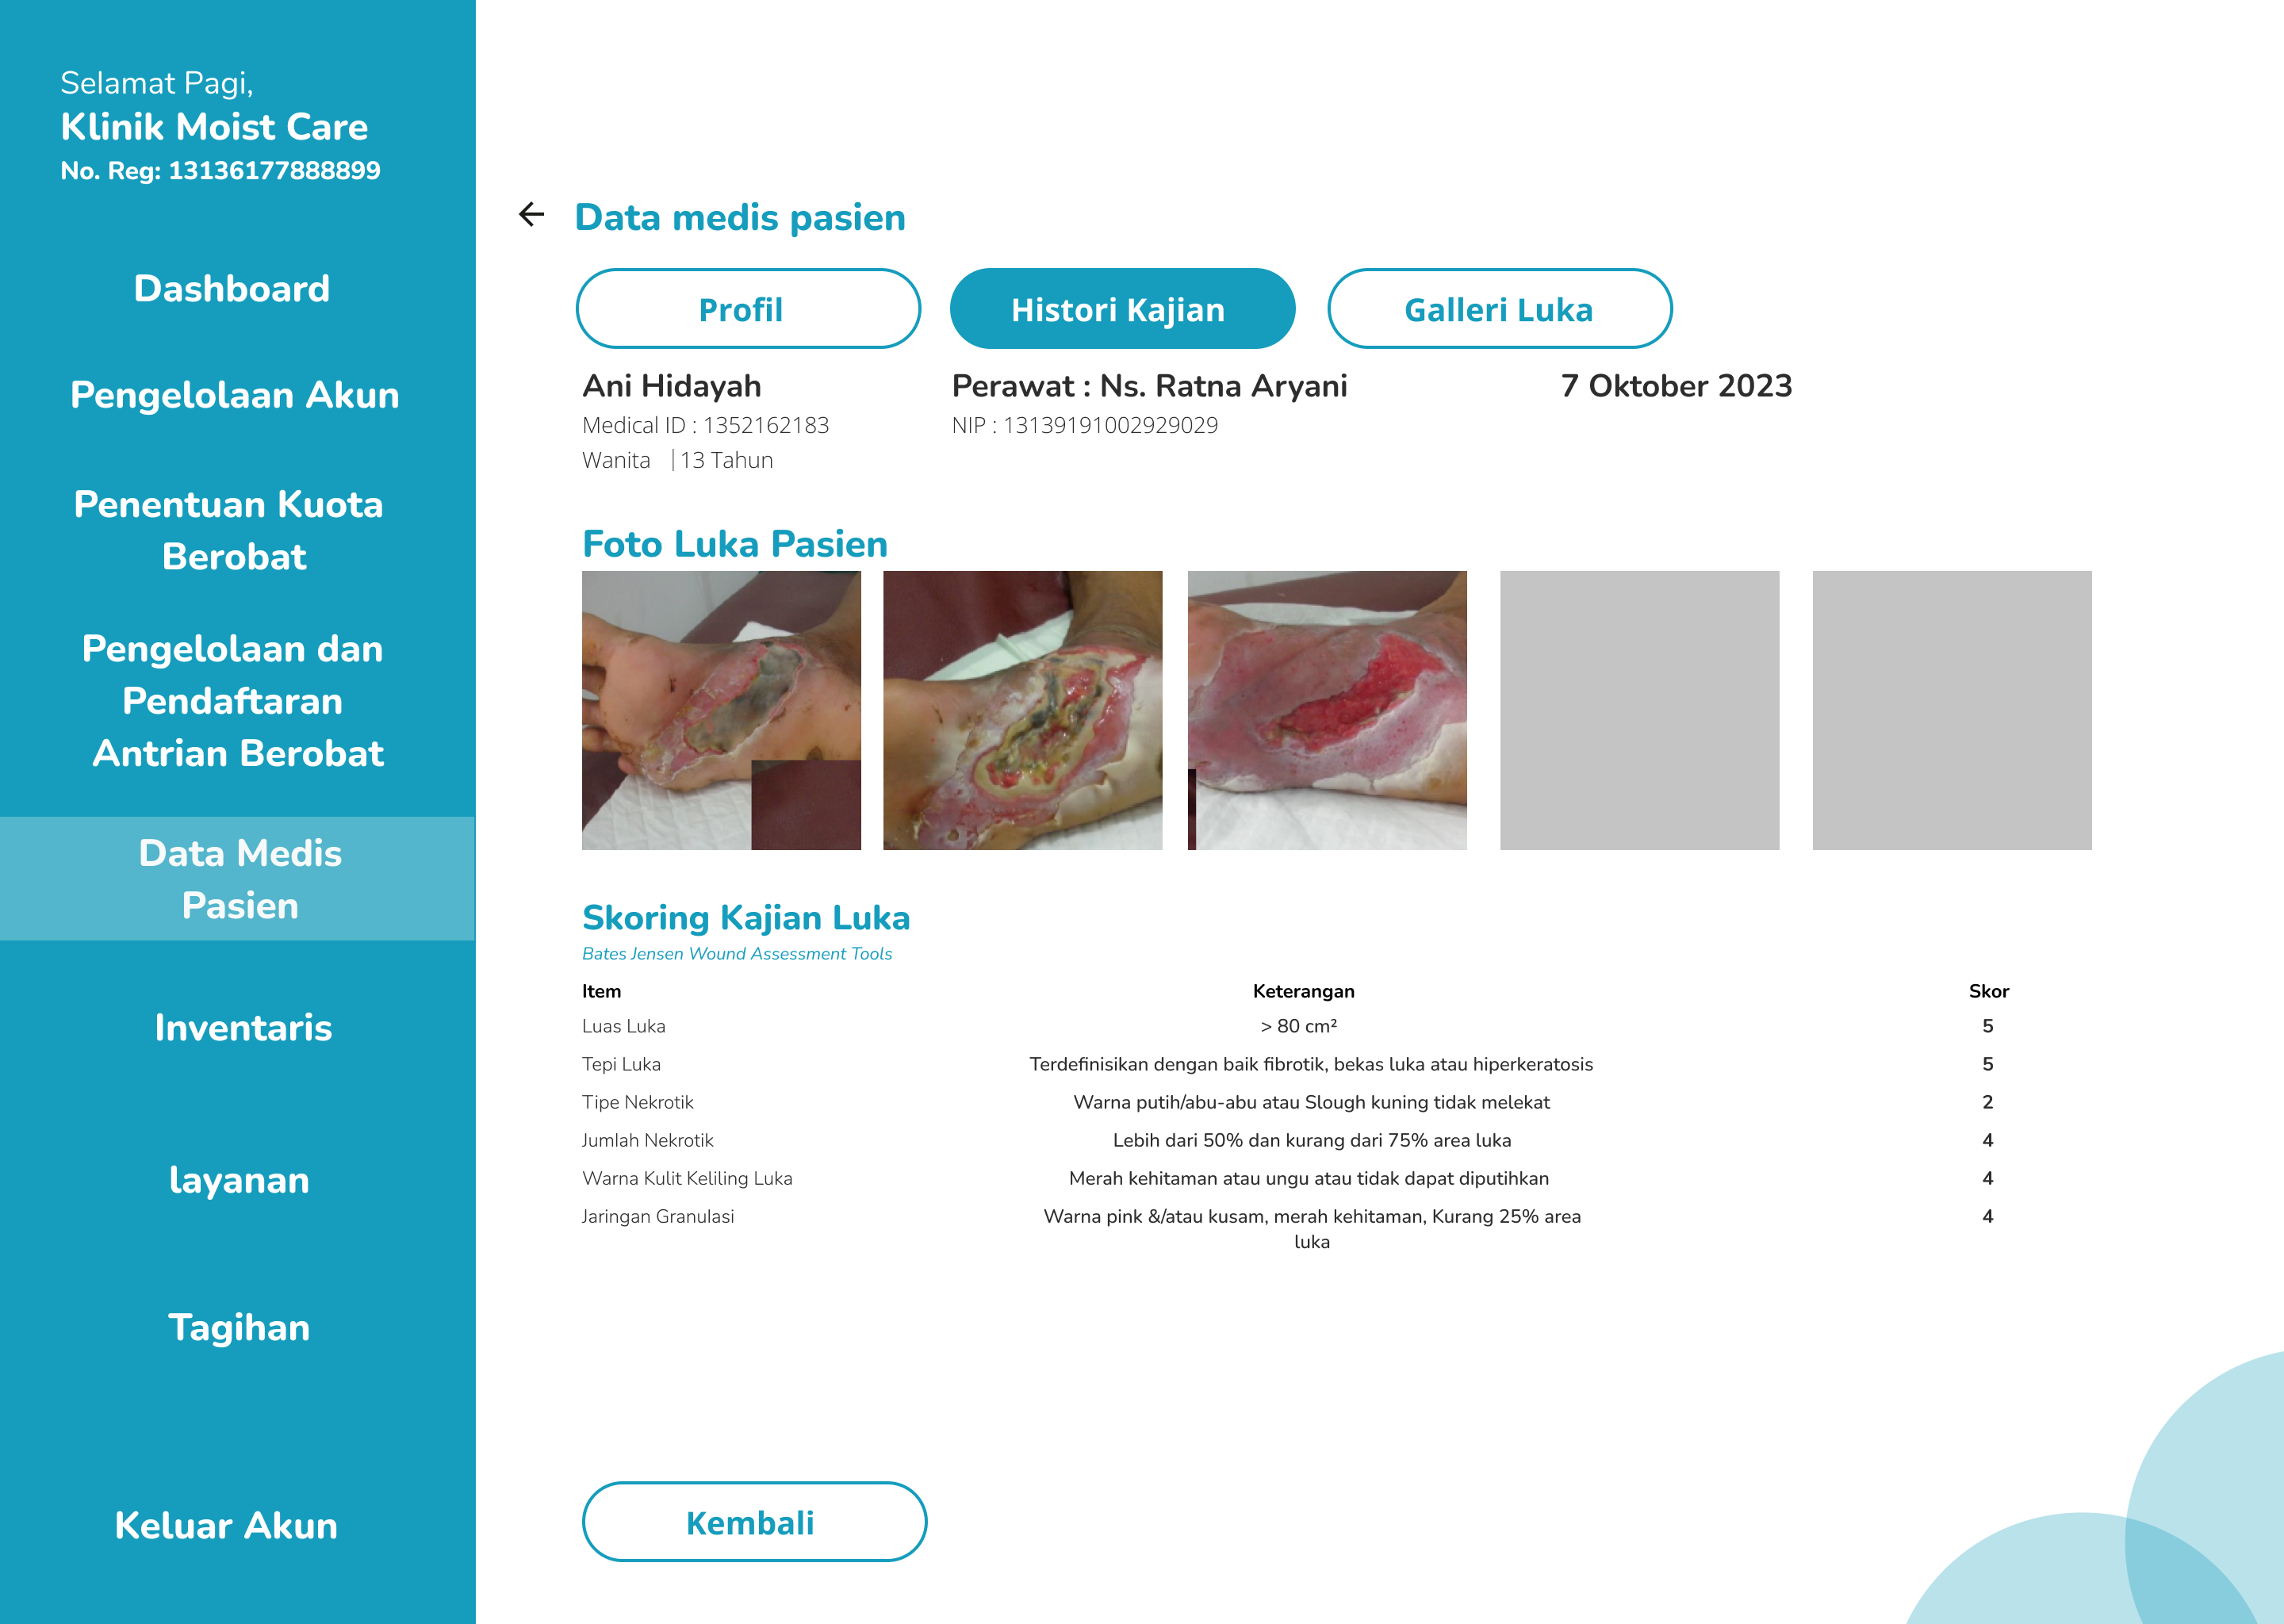
\includegraphics[width=12cm]{gambar/mockup_web/Proses Pengobatan 4.png}
		\caption{\emph{Mock up} detail histori kajian data medis pasien}
		\label{Gambar:pengelolaanantrian2}
	\end{figure}
	
	Ketika admin menekan tombol galeri luka \textbf{Gambar 4.8} maka akan diarahkan ke \textbf{Gambar 4.11} pada halaman selanjutnya yang merupakan galeri luka pasien dari semua histori kajian. Dan terdapat tombol kembali untuk menuju halaman sebelumnya.
	
	\begin{figure}[H]
		\centering
		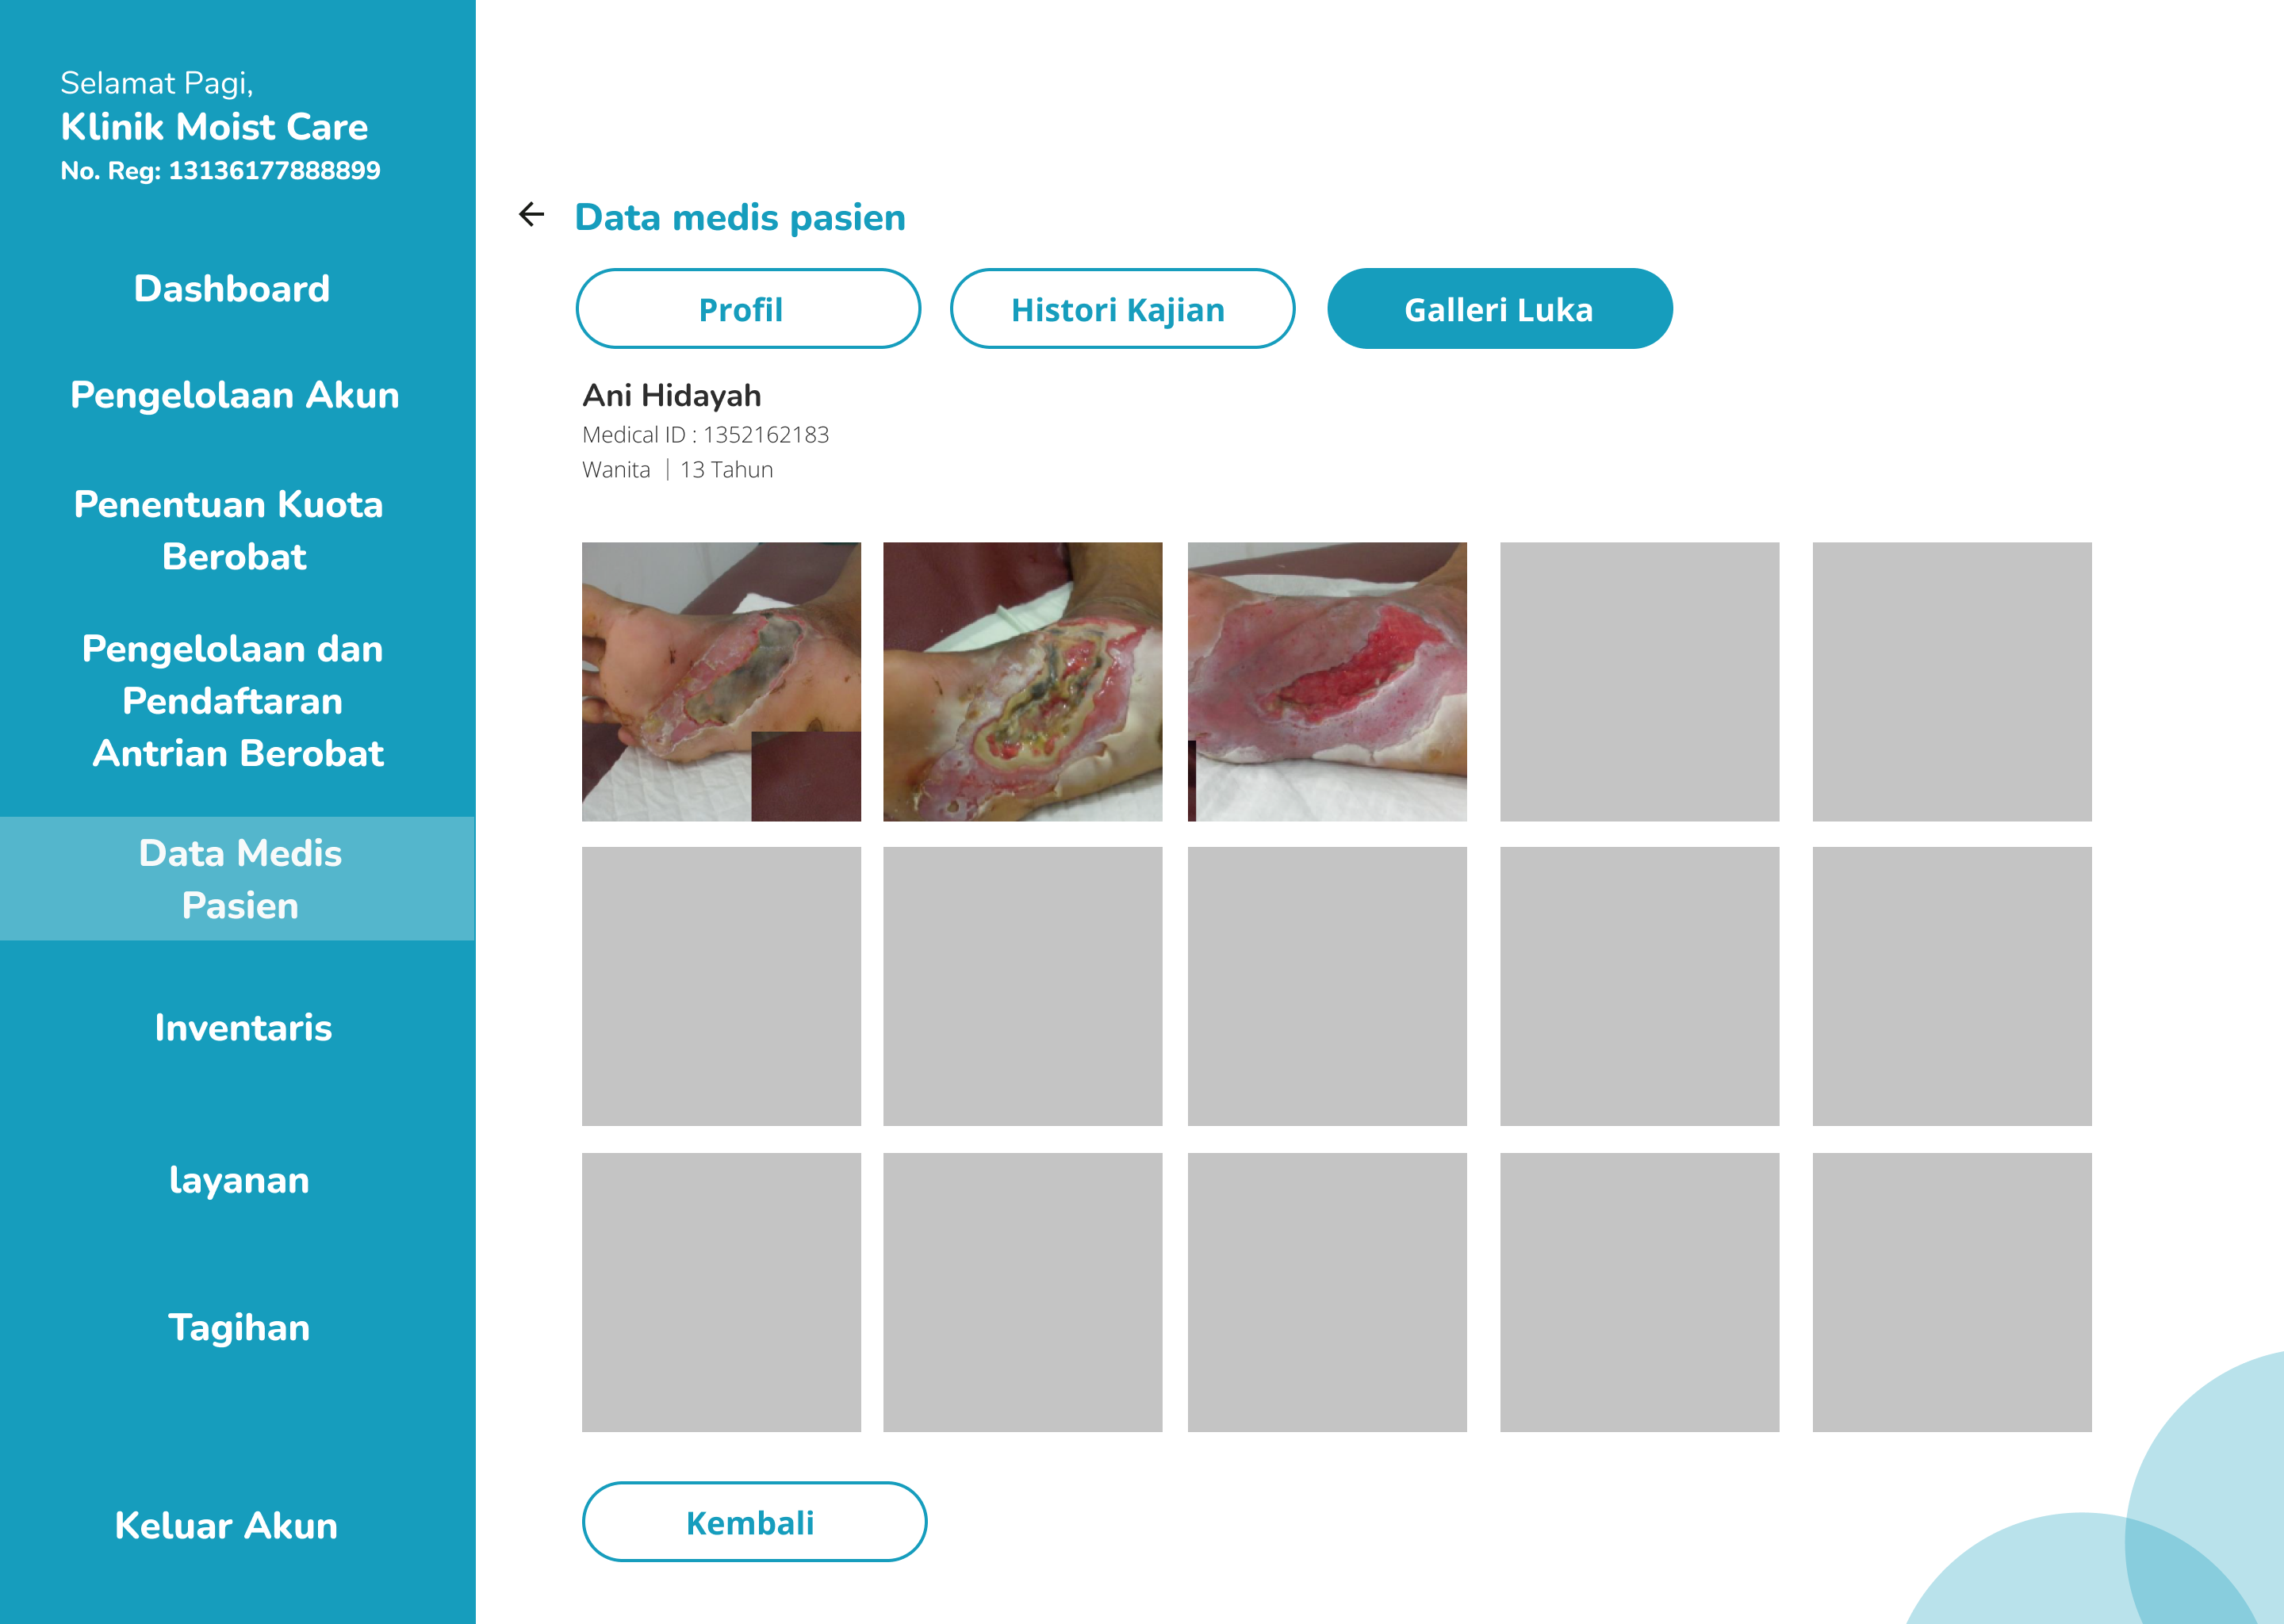
\includegraphics[width=12cm]{gambar/mockup_web/Proses Pengobatan 5.png}
		\caption{\emph{Mock up} galeri luka pasien}
		\label{Gambar:pengelolaanantrian2}
	\end{figure}
	
	\begin{figure}[H]
		\centering
		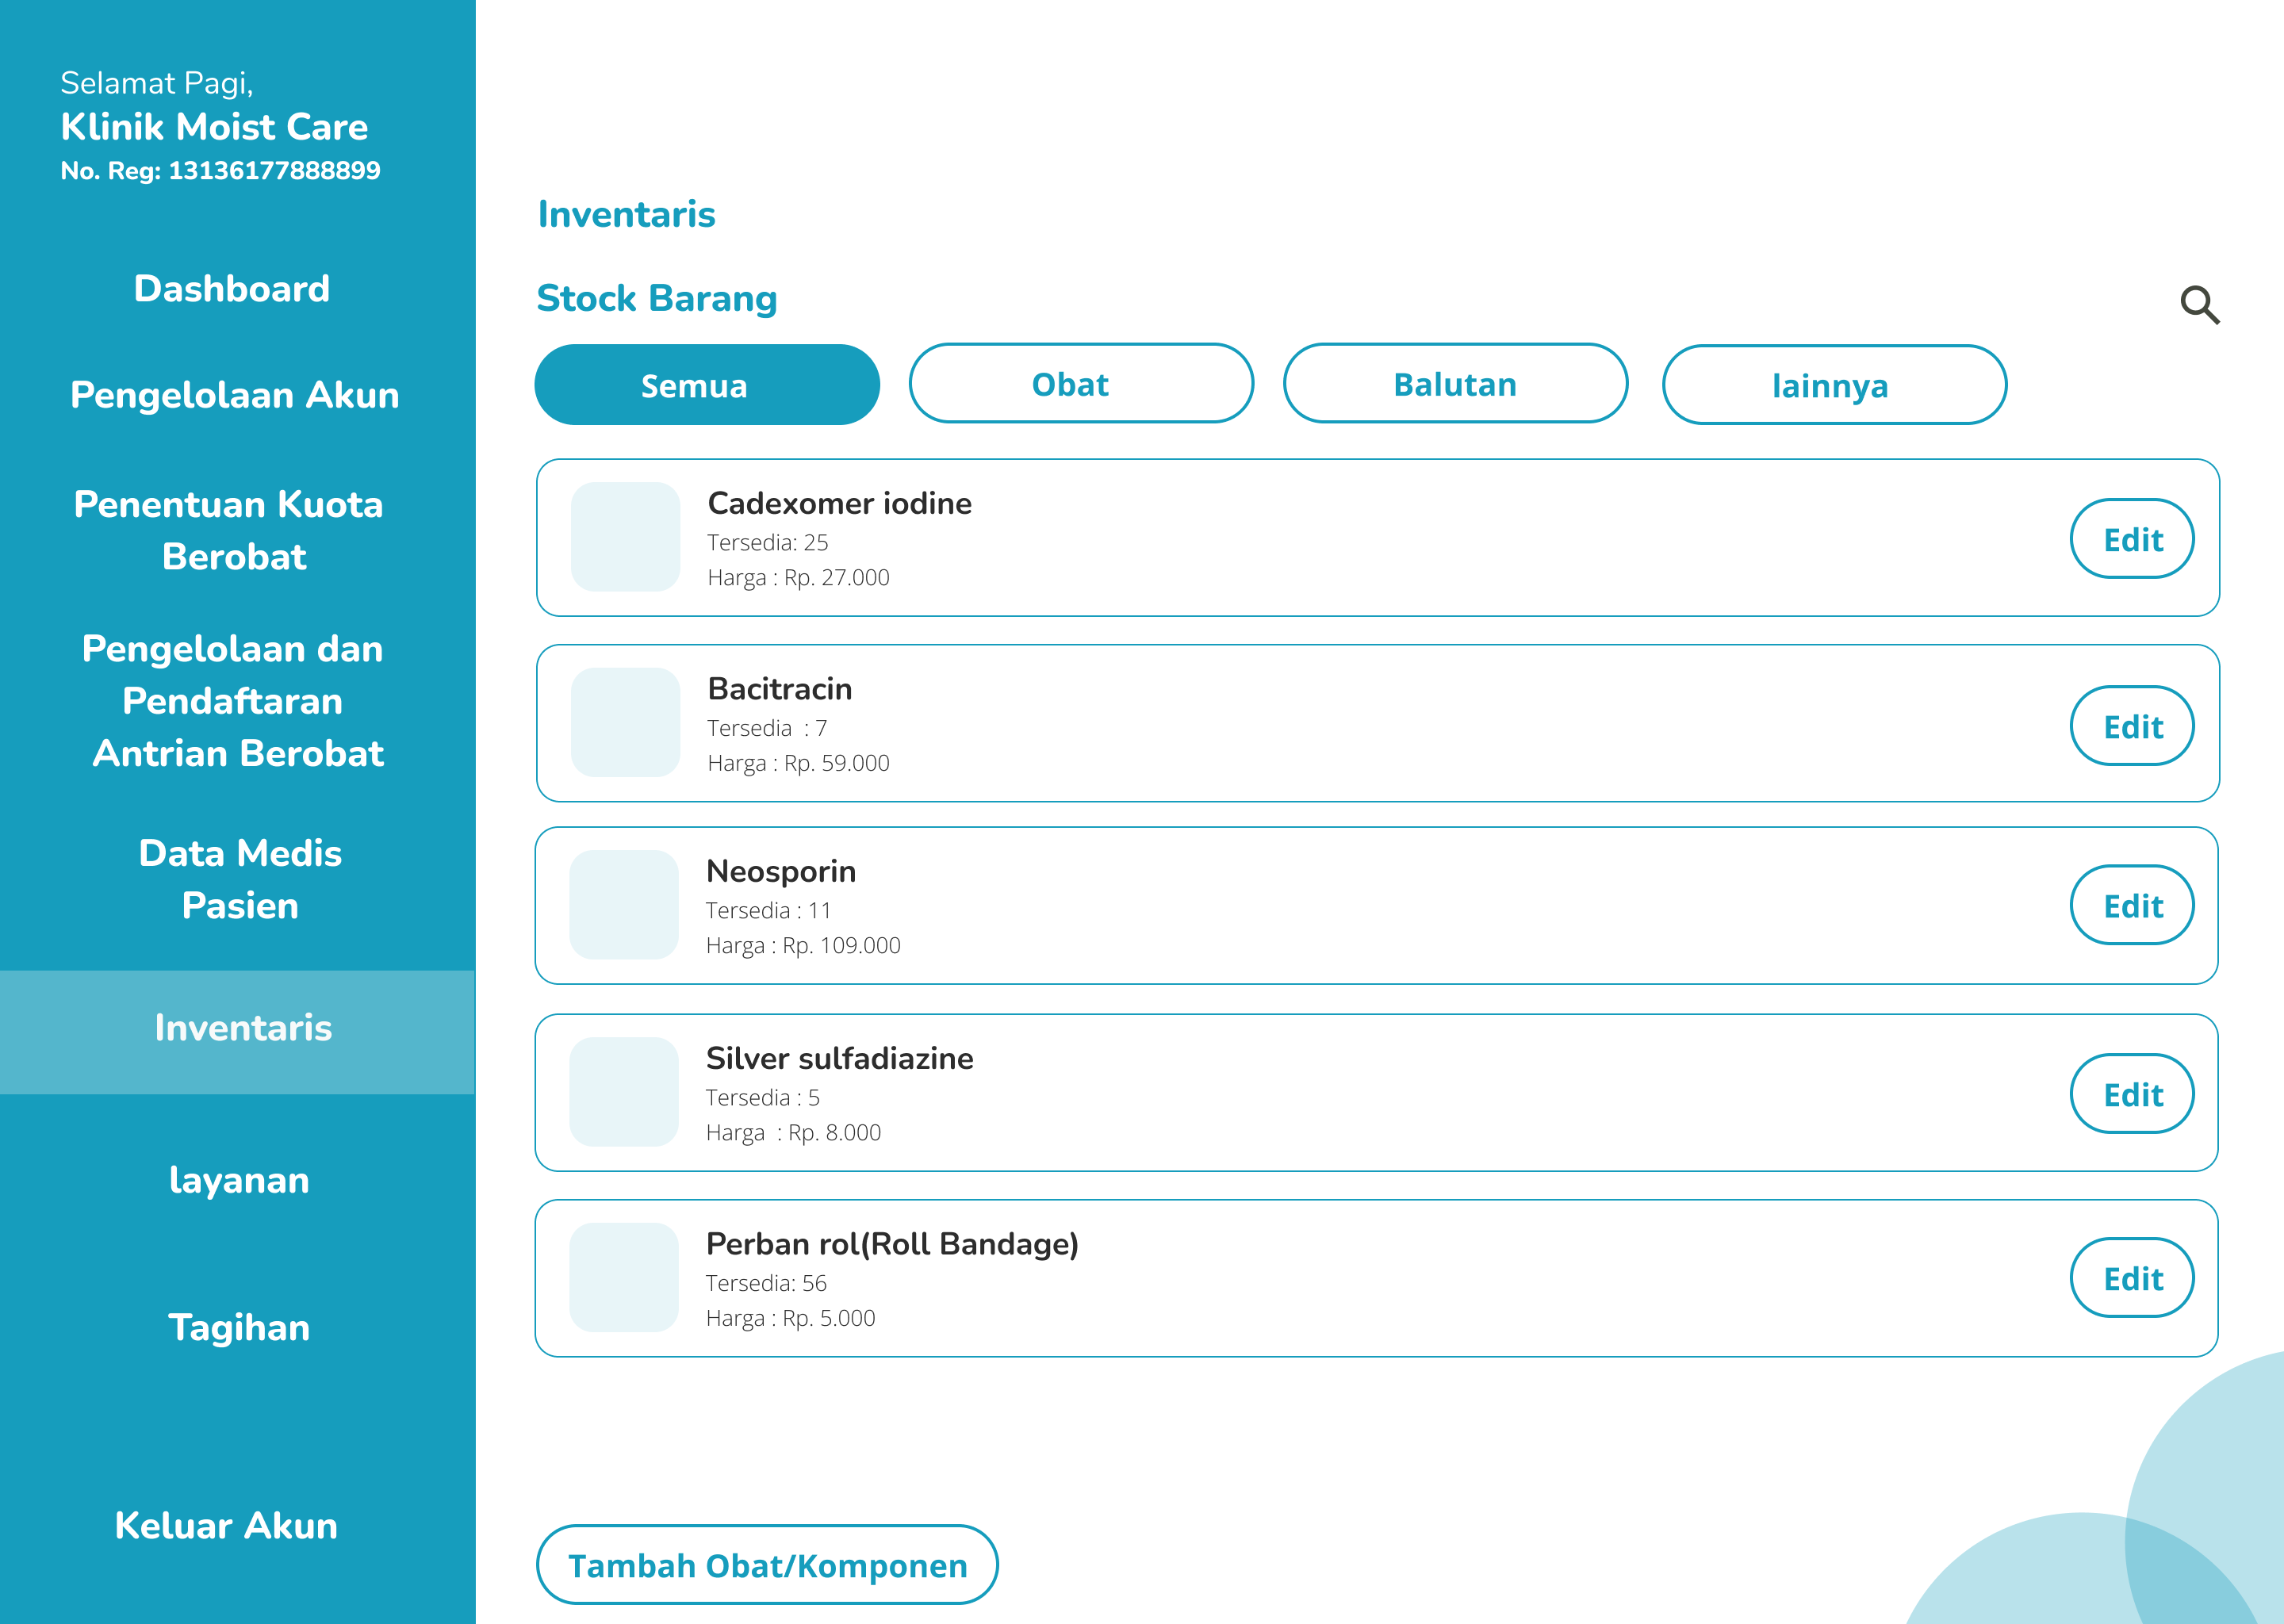
\includegraphics[width=12cm]{gambar/mockup_web/Inventaris1.png}
		\caption{\emph{Mock up} tampilan awal inventaris}
		\label{Gambar:pengelolaanantrian2}
	\end{figure}
	
	\textbf{Gambar 4.12} merupakan tampilan awal inventaris didalamnya terdapat \emph{list} barang berupa obat, balutan, dan komponen lainnya beserta detail stok, harganya dan tombol \emph{edit}. Terdapat juga tombol semua barang, obat, balutan, lainnya dan tambah obat/komponen.
	
	\begin{figure}[H]
		\centering
		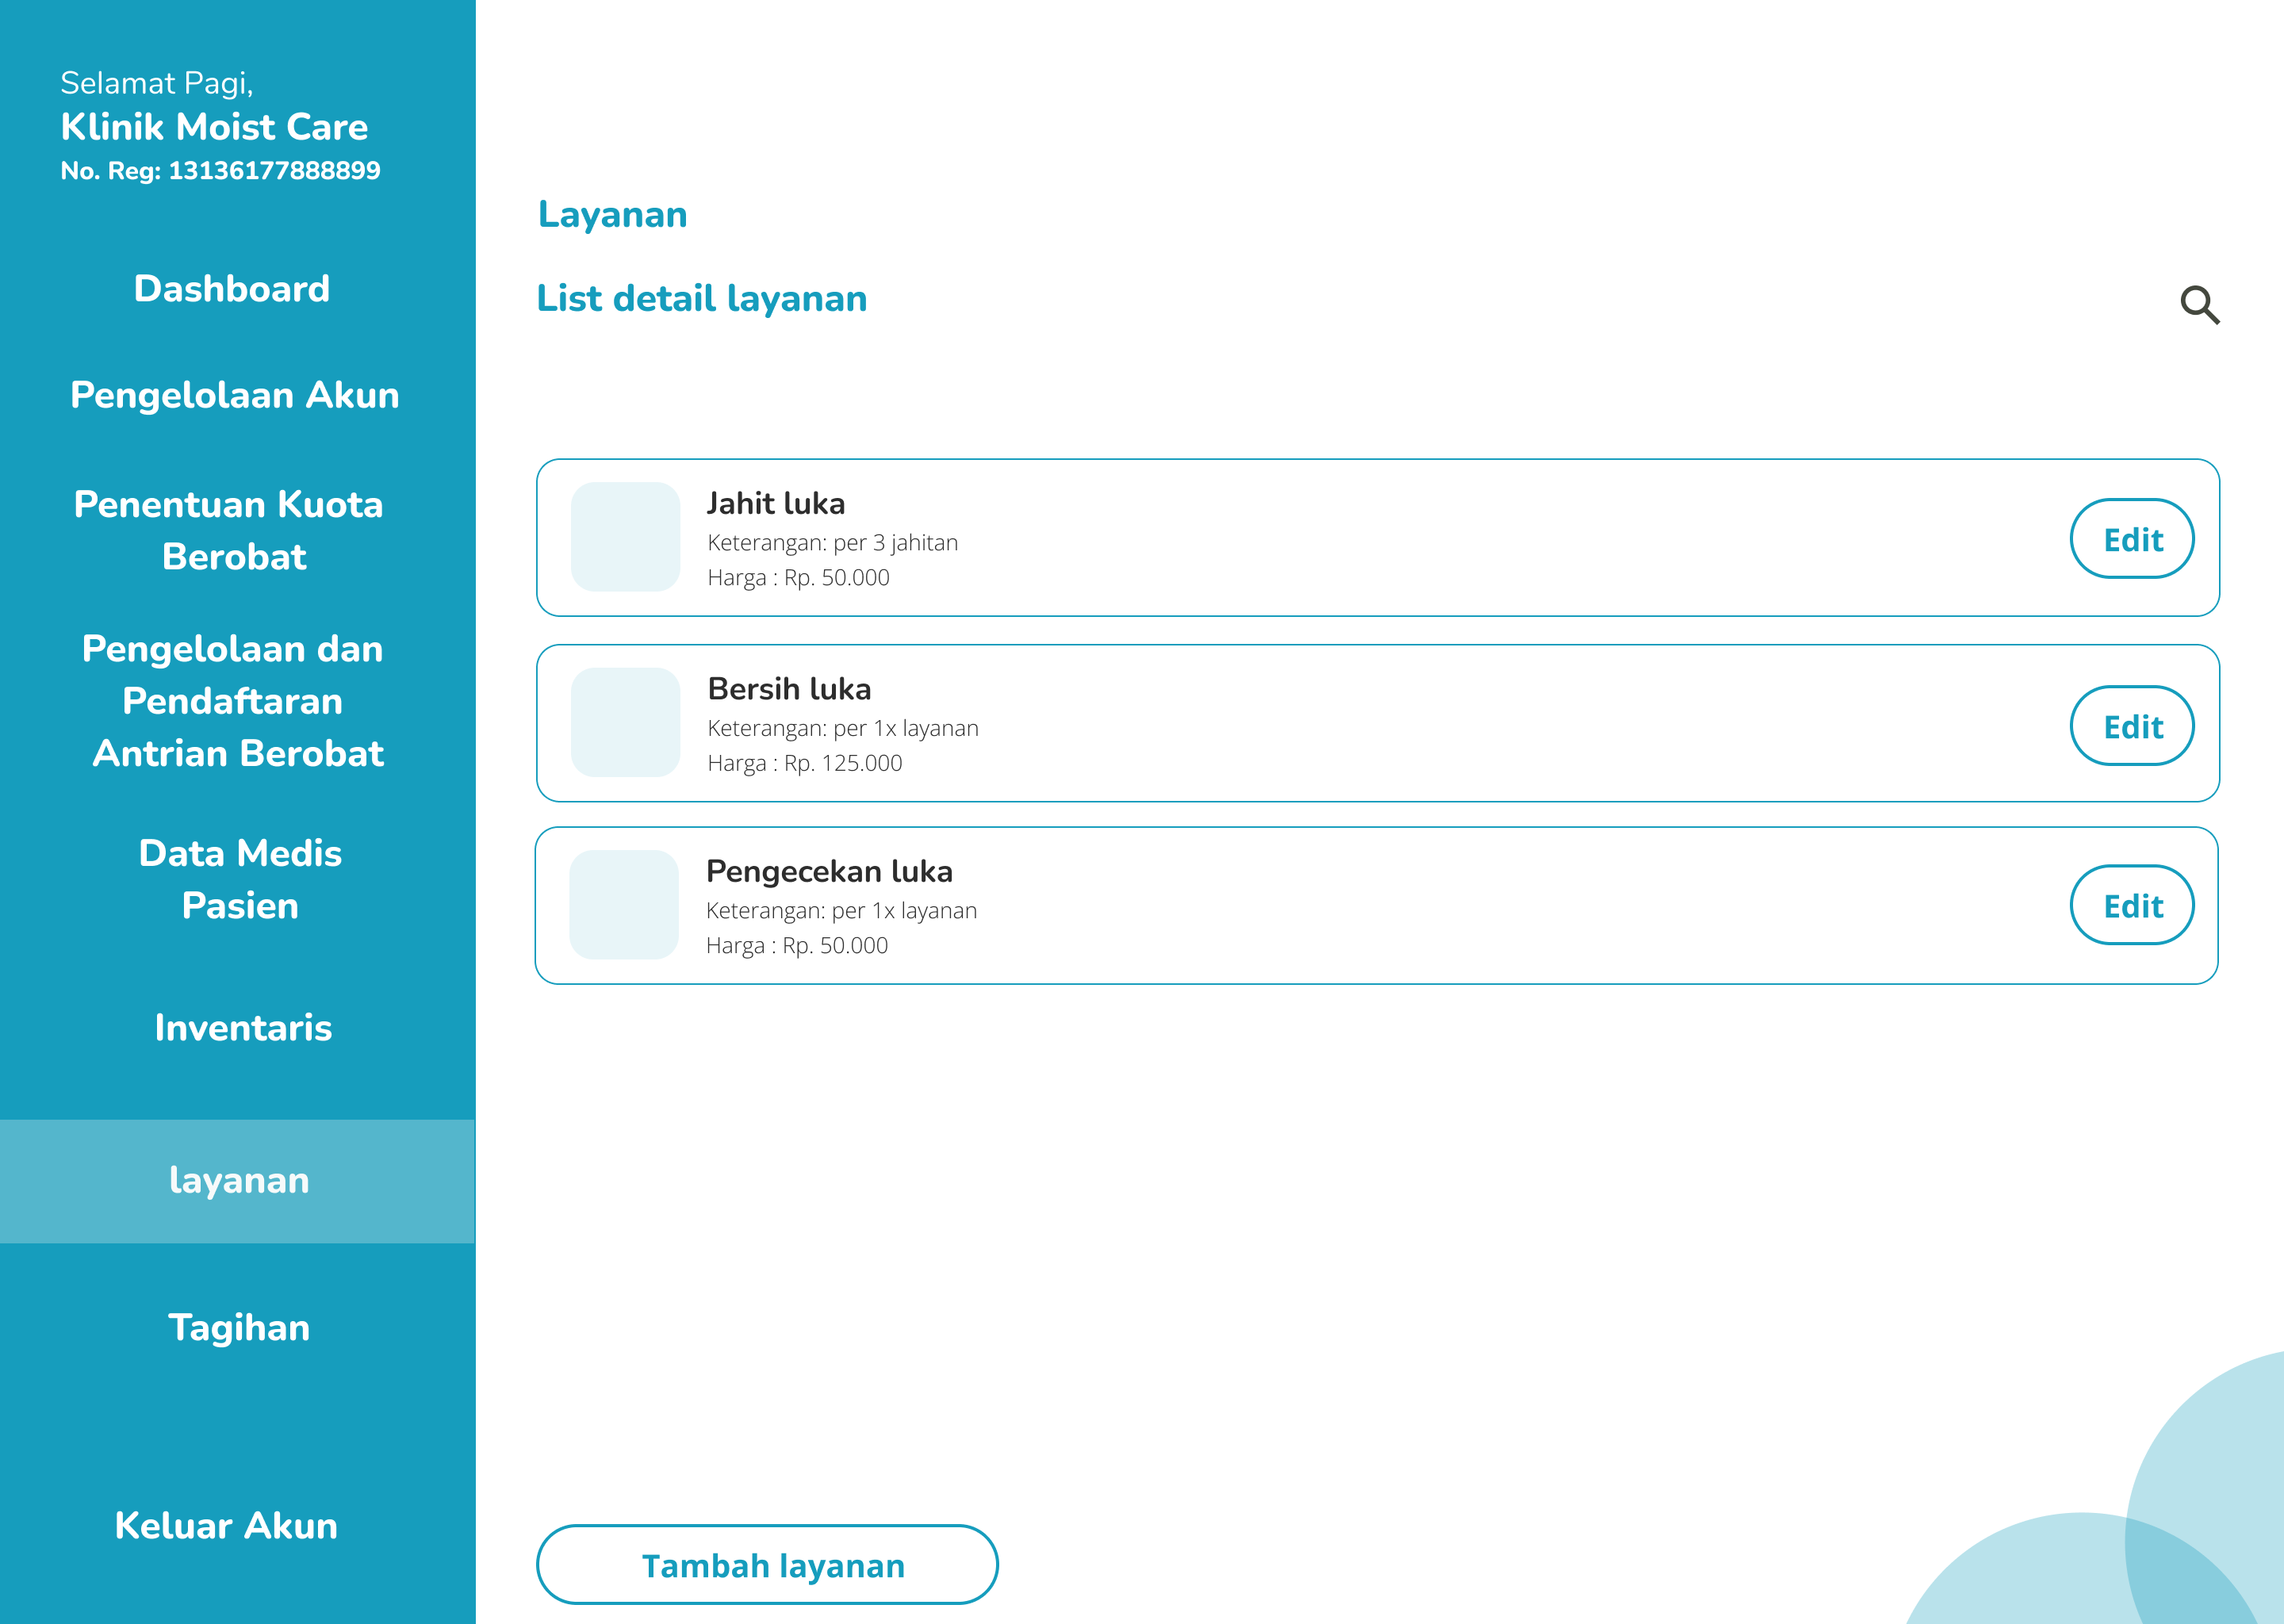
\includegraphics[width=12cm]{gambar/mockup_web/Layanan1.png}
		\caption{\emph{Mock up} tampilan awal layanan}
		\label{Gambar:pengelolaanantrian2}
	\end{figure}
	
	\textbf{Gambar 4.13} merupakan tampilan awal layanan didalamnya terdapat \emph{list} layanan beserta detail keterangana layanan, harganya dan tombol \emph{edit}.
	
	\break
	\item Desain \emph{routing table} proses pengobatan
	
	\textbf{Tabel 4.8}, \textbf{Tabel 4.9} dan \textbf{Tabel 4.10} merupakan \emph{routing table} untuk proses pengobatan:
	
	\begin{table}[H]
		\centering
		\caption{\emph{Routing table} proses pengobatan}
		\label{tabel_input}
		\begin{tabular}{|c|c|c|c|c|c|}
			\hline
			\textbf{\emph{Group}} & \textbf{\emph{Name}} & \textbf{API} & \textbf{HTTP} & \textbf{Keterangan} & \textbf{\emph{Return}} \\
			
			& & \textbf{\emph{Endpoint}} & \textbf{\emph{Verb}} & & \textbf{\emph{Type}} \\
			\hline
			
			Pengo- & 
			\emph{READ} &
			/data\_kajians&
			\emph{GET} &
			Menampilkan halaman &
			\emph{view}\\
			
			
			batan& 
			&
			&
			&
			data kajian semua &\\
			
			& 
			&
			&
			&
			pasien berdasarkan nama &\\
			
			& 
			&
			&
			&
			pasien &\\
			\hline
			
			& 
			\emph{READ} &
			/data\_kajians&
			\emph{GET} &
			Menampilkan data &
			\{<nip>,\\
			
			
			& 
			&
			/<nip>&
			&
			kajian semua pasien &
			<nama\_\\
			
			& 
			&
			&
			&
			berdasarkan nama &
			pegawai>,\\
			
			& 
			&
			&
			&
			perawat &
			<nrm>,\\
			
			& 
			&
			&
			&
			&
			<nama\_\\
			
			& 
			&
			&
			&
			&
			pasien>\}\\
			\hline
			
			& 
			\emph{READ} &
			/data\_kajians&
			\emph{GET} &
			Menampilkan data &
			\{<nrm>,\\
			
			
			& 
			&
			/<nrm>&
			&
			kajian semua pasien&
			<nama\_\\
			
			& 
			&
			&
			&
			berdasarkan nomor &
			pasien>\}\\
			
			& 
			&
			&
			&
			rekam medis &
			\\
			\hline
			
			& 
			\emph{READ} &
			/profil\_&
			\emph{GET} &
			Menampilkan halaman &
			\emph{view}\\
			
			
			& 
			&
			pasien&
			&
			profil 1 pasien &
			\\
			
			& 
			&
			/<nrm>&
			&
			berdasarkan NRM &
			\\
			\hline
			
		\end{tabular}
	\end{table}
	
	\begin{table}[H]
		\centering
		\caption{\emph{Routing table} proses pengobatan - lanjutan 1}
		\label{tabel_input}
		\begin{tabular}{|c|c|c|c|c|c|}
			\hline
			\textbf{\emph{Group}} & \textbf{\emph{Name}} & \textbf{API} & \textbf{HTTP} & \textbf{Keterangan} & \textbf{\emph{Return}} \\
			
			& & \textbf{\emph{Endpoint}} & \textbf{\emph{Verb}} & & \textbf{\emph{Type}} \\
			\hline
			
			Pengo-& 
			\emph{READ} &
			/\emph{list}\_data&
			\emph{GET} &
			Menampilkan &
			\emph{view}\\
			
			
			batan& 
			&
			\_kajian&
			&
			halaman \emph{list} histori&
			\\
			
			& 
			&
			/<nrm>&
			&
			 kajian 1 pasien&
			\\
			
			& 
			&
			&
			&
			berdasarkan NRM  &
			\\
			\hline
			
			& 
			\emph{READ} &
			/galeri\_luka&
			\emph{GET} &
			Menampilkan  &
			\emph{view}\\
			
			
			& 
			&
			/<nrm>&
			&
			halaman galeri luka  &
			\\
			
			& 
			&
			&
			&
			pasien berdasarkan&
			\\
			
			& 
			&
			&
			&
			NRM&
			\\
		
			\hline
			
			Inven& 
			\emph{READ} &
			/\emph{list}\_&
			\emph{GET} &
			Menampilkan&
			\emph{view}\\
			
			
			-taris& 
			&
			inventaris&
			&
			halaman \emph{list}&
			\\
			
			& 
			&
			&
			&
			semua inventaris&
			\\
			\hline
			
			& 
			\emph{CREATE} &
			/\emph{add}\_&
			\emph{POST} &
			Menampilkan &
			\emph{view}\\
			
			& 
			&
			inventaris&
			&
			halaman tambah&
			\\
			
			& 
			&
			&
			&
			inventaris&
			\\
			\hline
			
			& 
			\emph{UPDATE} &
			/\emph{edit}\_&
			\emph{POST} &
			Menampilkan &
			\emph{view}\\
			
			& 
			&
			inventaris&
			&
			halaman \emph{edit} &
			\\
			
			& 
			&
			/<\_id>&
			&
			inventaris &
			\\
			\hline
			
			& 
			\emph{DESTROY} &
			/\emph{delete}\_&
			\emph{DELETE} &
			Hapus data &
			\emph{view}\\
			
			& 
			&
			inventaris&
			&
			inventaris &
			\\
			
			& 
			&
			/<\_id>&
			&
			&
			\\
			
			\hline
			
			Laya & 
			\emph{READ} &
			/\emph{list}\_ &
			\emph{GET} &
			Menampilkan &
			\emph{view}\\
			
			-nan& 
			&
			layanan&
			&
			halaman \emph{list} &
			\\
			
			& 
			&
			&
			&
			semua layanan &
			\\
			\hline
			
		\end{tabular}
	\end{table}
	
	\begin{table}[H]
		\centering
		\caption{\emph{Routing table} proses pengobatan - lanjutan 2}
		\label{tabel_input}
		\begin{tabular}{|c|c|c|c|c|c|}
			\hline
			\textbf{\emph{Group}} & \textbf{\emph{Name}} & \textbf{API} & \textbf{HTTP} & \textbf{Keterangan} & \textbf{\emph{Return}} \\
			
			& & \textbf{\emph{Endpoint}} & \textbf{\emph{Verb}} & & \textbf{\emph{Type}} \\
			\hline
	
			Laya-& 
			\emph{CREATE} &
			/\emph{add}\_&
			\emph{POST} &
			Menampilkan&
			\emph{view}\\
			
			nan& 
			&
			layanan&
			&
			halaman tambah&
			\\
			
			& 
			&
			&
			&
			layanan&
			\\
			\hline
			
			& 
			\emph{UPDATE} &
			/\emph{edit}&
			\emph{POST} &
			Menampilkan&
			\emph{view}\\
			
			& 
			&
			\_layanan&
			&
			halaman \emph{edit}&
			\\
			
			& 
			&
			/<\_id>&
			&
			layanan&
			\\
			\hline
			
			& 
			\emph{DESTROY} &
			/\emph{delete}&
			\emph{DELETE} &
			Hapus&
			\emph{view}\\
			
			& 
			&
			\_layanan&
			&
			layanan &
			\\
			
			& 
			&
			<\_id>&
			&
			&
			\\
			\hline
			
		\end{tabular}
	\end{table}
	
	\item Membuat \emph{database} proses pengobatan
	
	\begin{figure}[H]
		\centering
		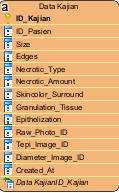
\includegraphics[width=4cm]{gambar/data_kajian_database.png}
		\caption{Tabel data kajian}
		\label{Gambar:pengelolaanantrian2}
	\end{figure}

	\textbf{Gambar 4.14} merupaka data kajian memuat beberapa atribut yaitu id\_kajian, \emph{size}, \emph{edges}, \emph{necrotic\_type}, \emph{necrotic\_amount}, \emph{skincolor\_surround}, \emph{granulation\_tissue}, \emph{epithelization}, raw\_\emph{photo}\_id, tipe\_\emph{image}\_id, diameter\_\emph{image}, dan \emph{created\_at}. Data tersebut akan disimpan pada \emph{database} MongoDB dan disimpan dalam format JSON.
	
	\begin{figure}[H]
		\centering
		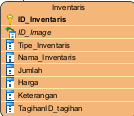
\includegraphics[width=4cm]{gambar/inventaris_database.png}
		\caption{Tabel inventaris}
		\label{Gambar:pengelolaanantrian2}
	\end{figure}

	\textbf{Gambar 4.15} merupakan tabel inventaris memuat beberapa atribut yaitu id\_inventaris, id\_\emph{image}, tipe\_inventaris, nama\_inventaris, jumlah, harga, dan keterangan. Data tersebut akan disimpan pada \emph{database} MongoDB dan disimpan dalam format JSON.

	\begin{figure}[H]
		\centering
		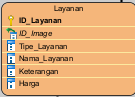
\includegraphics[width=4cm]{gambar/layanan_database.png}
		\caption{Tabel layanan}
		\label{Gambar:pengelolaanantrian2}
	\end{figure}
	
	\textbf{Gambar 4.16} merupakan tabel layanan memuat beberapa atribut yaitu id\_layanan, id\_\emph{image}, tipe\_layanan, nama\_layanan, keterangan, dan harga. Data tersebut akan disimpan pada \emph{database} MongoDB dan disimpan dalam format JSON.
	
	\item Pembuatan \emph{mock up} pendaftaran pasien berobat
	
	Pada \textbf{Gambar 4.17} di halaman selanjutnya merupakan tampilan \emph{live} yang berisi  antrian berobat lengkap beserta nama pasien dan nomor antrian.
	
	\begin{figure}[H]
		\centering
		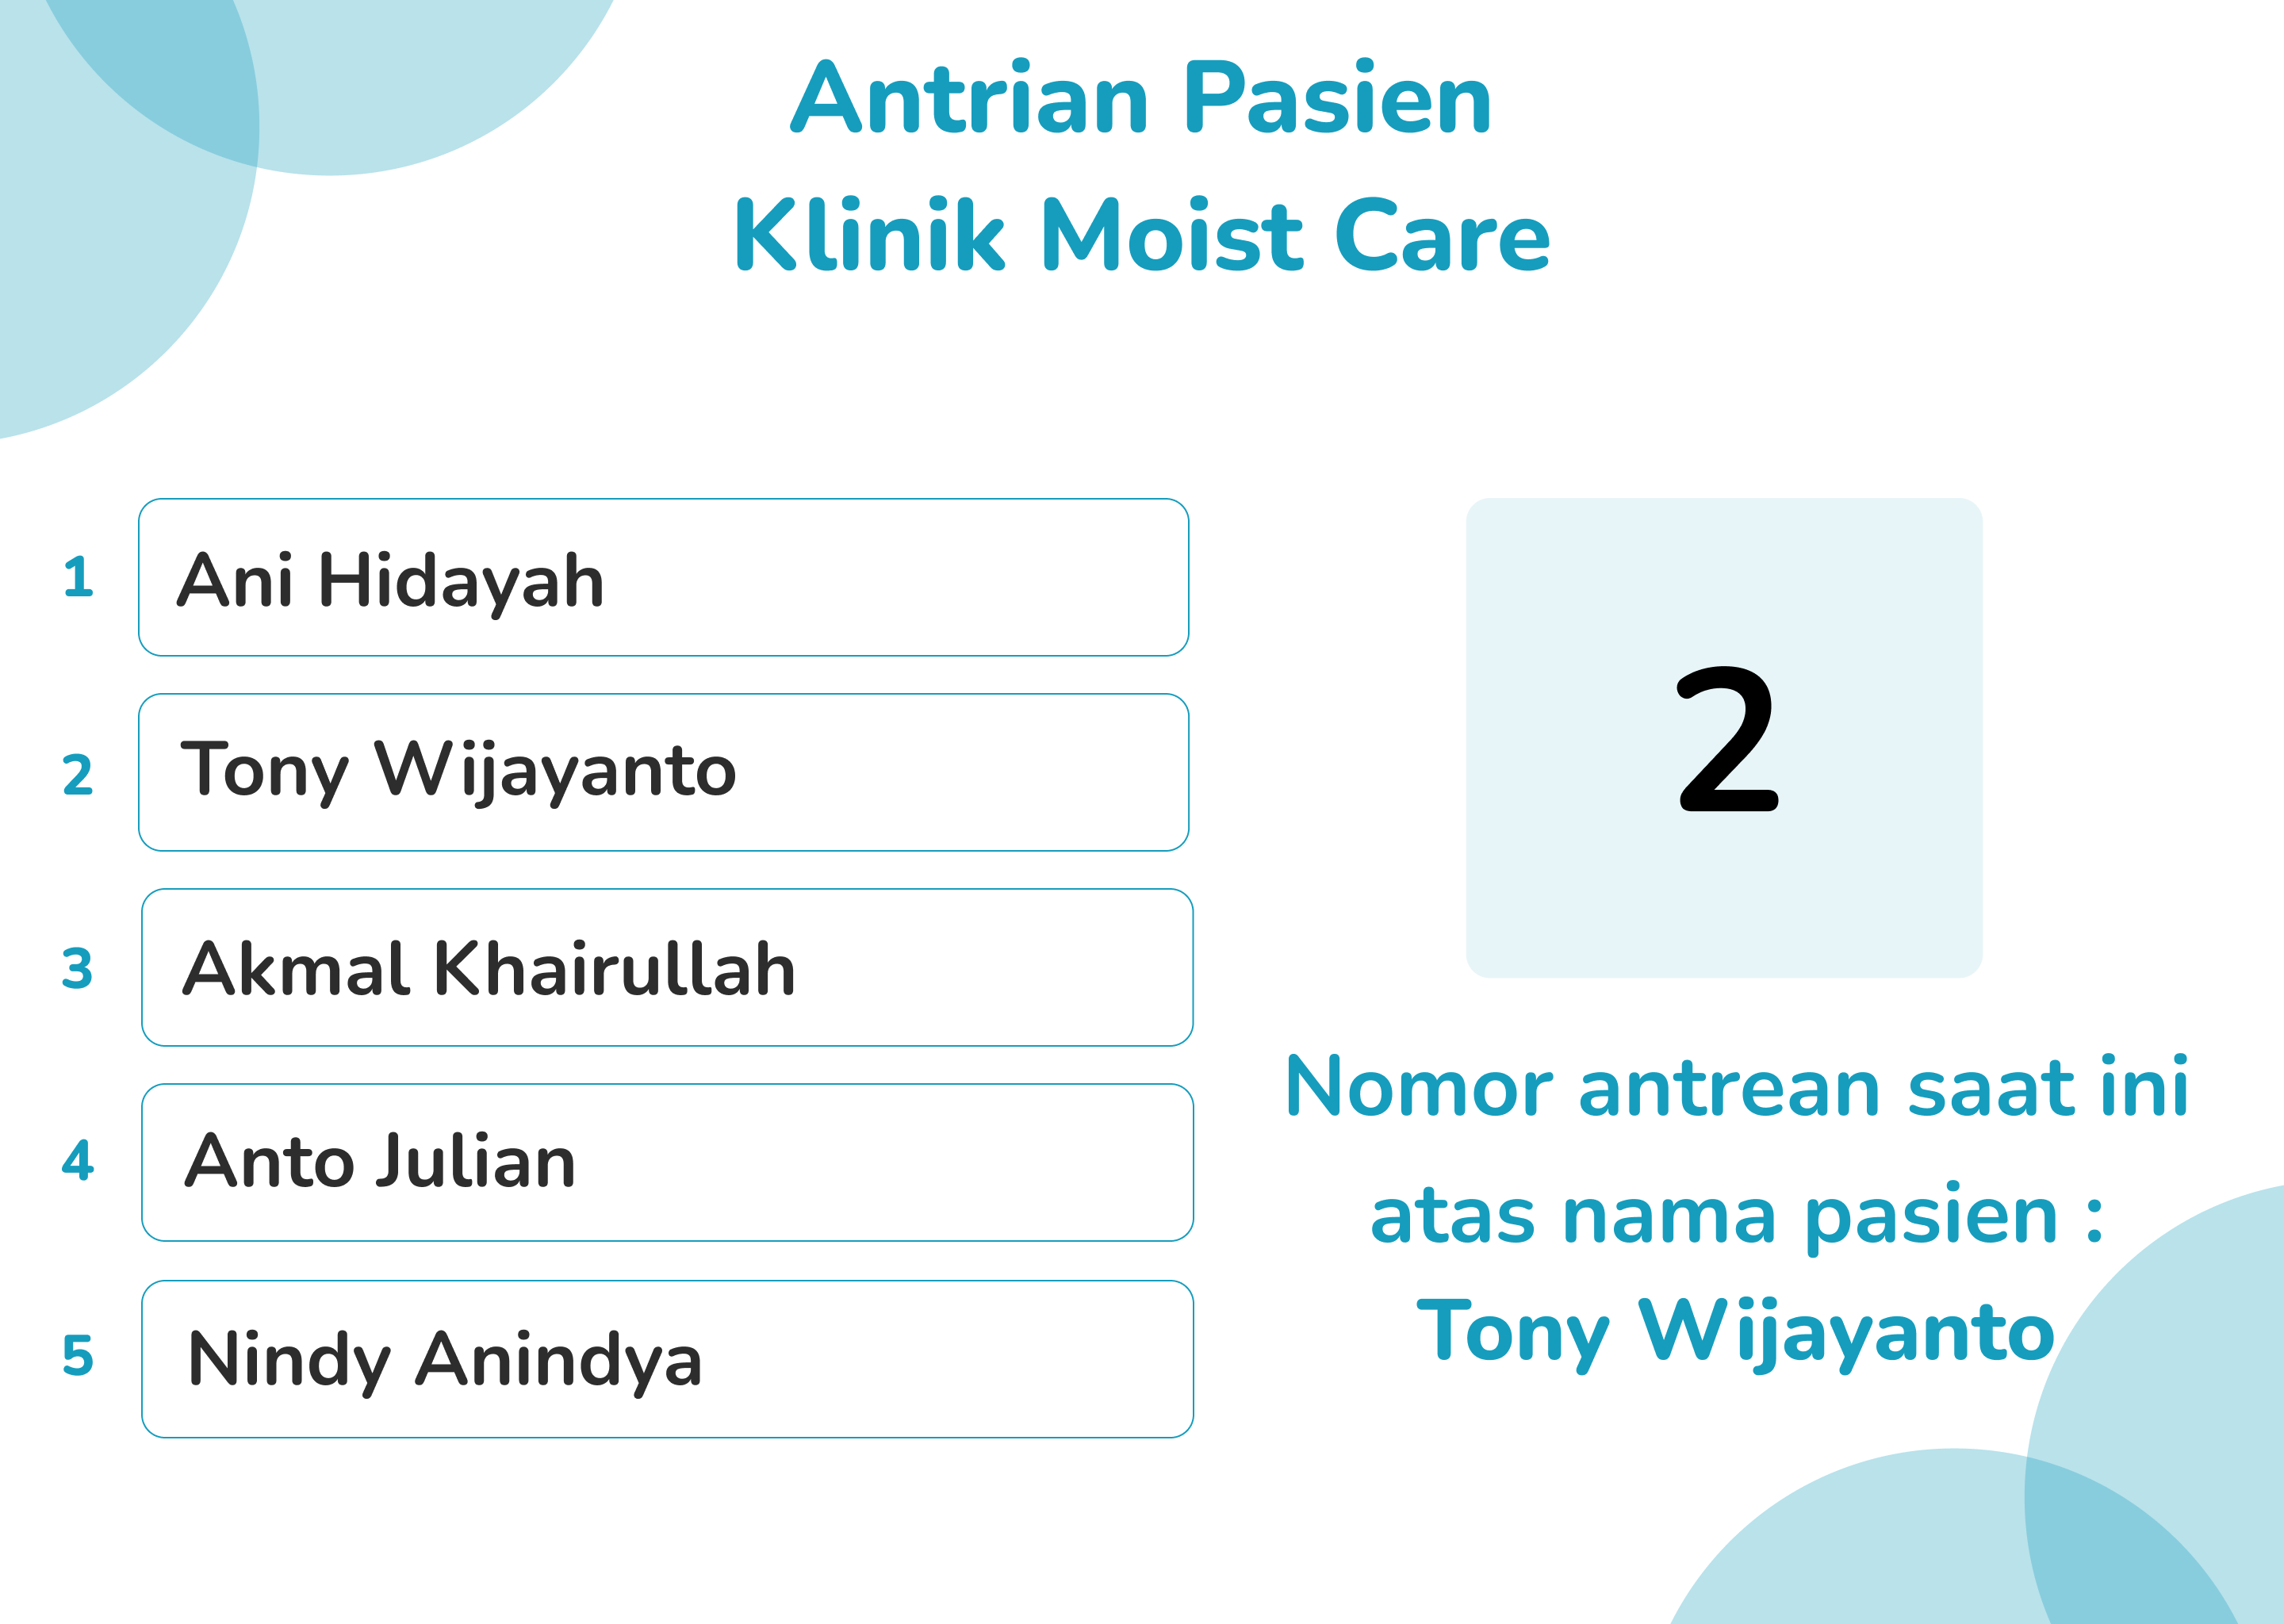
\includegraphics[width=12cm]{gambar/mockup_web/Pendaftaran Akun Berobat.png}
		\caption{\emph{Mock up} melihat daftar dan urutan pasien yang akan dilayani}
		\label{Gambar:pendaftaranakunberobat1}
	\end{figure}
	
	\item Desain \emph{routing table} pendaftaran pasien berobat. 
	
	\textbf{Tabel 4.11} merupakan \emph{routing table} untuk pendaftaran pasien berobat:
	
	\begin{table}[H]
		\centering
		\caption{\emph{Routing table} pendaftaran pasien berobat}
		\label{tabel_input}
		\begin{tabular}{|c|c|c|c|c|c|}
			\hline
			\textbf{\emph{Group}} & \textbf{\emph{Name}} & \textbf{API} & \textbf{HTTP} & \textbf{Keterangan} & \textbf{\emph{Return}} \\
			
			& & \textbf{\emph{Endpoint}} & \textbf{\emph{Verb}} & & \textbf{\emph{Type}} \\
			\hline
			
			& 
			\emph{READ} &
			/antrian&
			\emph{GET} &
			Menampilkan halaman&
			\emph{view}\\
			
			
			& 
			&
			\emph{\_real\_time}&
			&
			daftar dan urutan pasien&\\
			
			& 
			&
			&
			&
			yang akan dilayani &\\
			\hline
			
		\end{tabular}
	\end{table}
	
	\item Membuat \emph{database} pendaftaran pasien berobat
	
	\textbf{Gambar 4.18} pada halaman selanjutnya merupakan tabel detail tagihan memuat beberapa atribut yaitu id\_pendaftaran, tipe\_pendaftaran, id\_pasien dan \emph{created\_at}. Data tersebut akan disimpan pada \emph{database} MongoDB dan disimpan dalam format JSON.
	
	\begin{figure}[H]
		\centering
		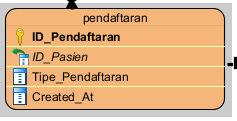
\includegraphics[width=6cm]{gambar/Pendaftaran_database.png}
		\caption{Tabel pendaftaran berobat}
		\label{Gambar:pengelolaanantrian1}
	\end{figure}
	
	\item Pembuatan \emph{mock up} pengelolaan antrian
	
	\textbf{Gambar 4.19} merupakan tampilan menentukan kuota pelayanan pasien yang mendaftar secara \emph{offline} maupun \emph{online} pada hari yang ditentukan.
	
	\begin{figure}[H]
		\centering
		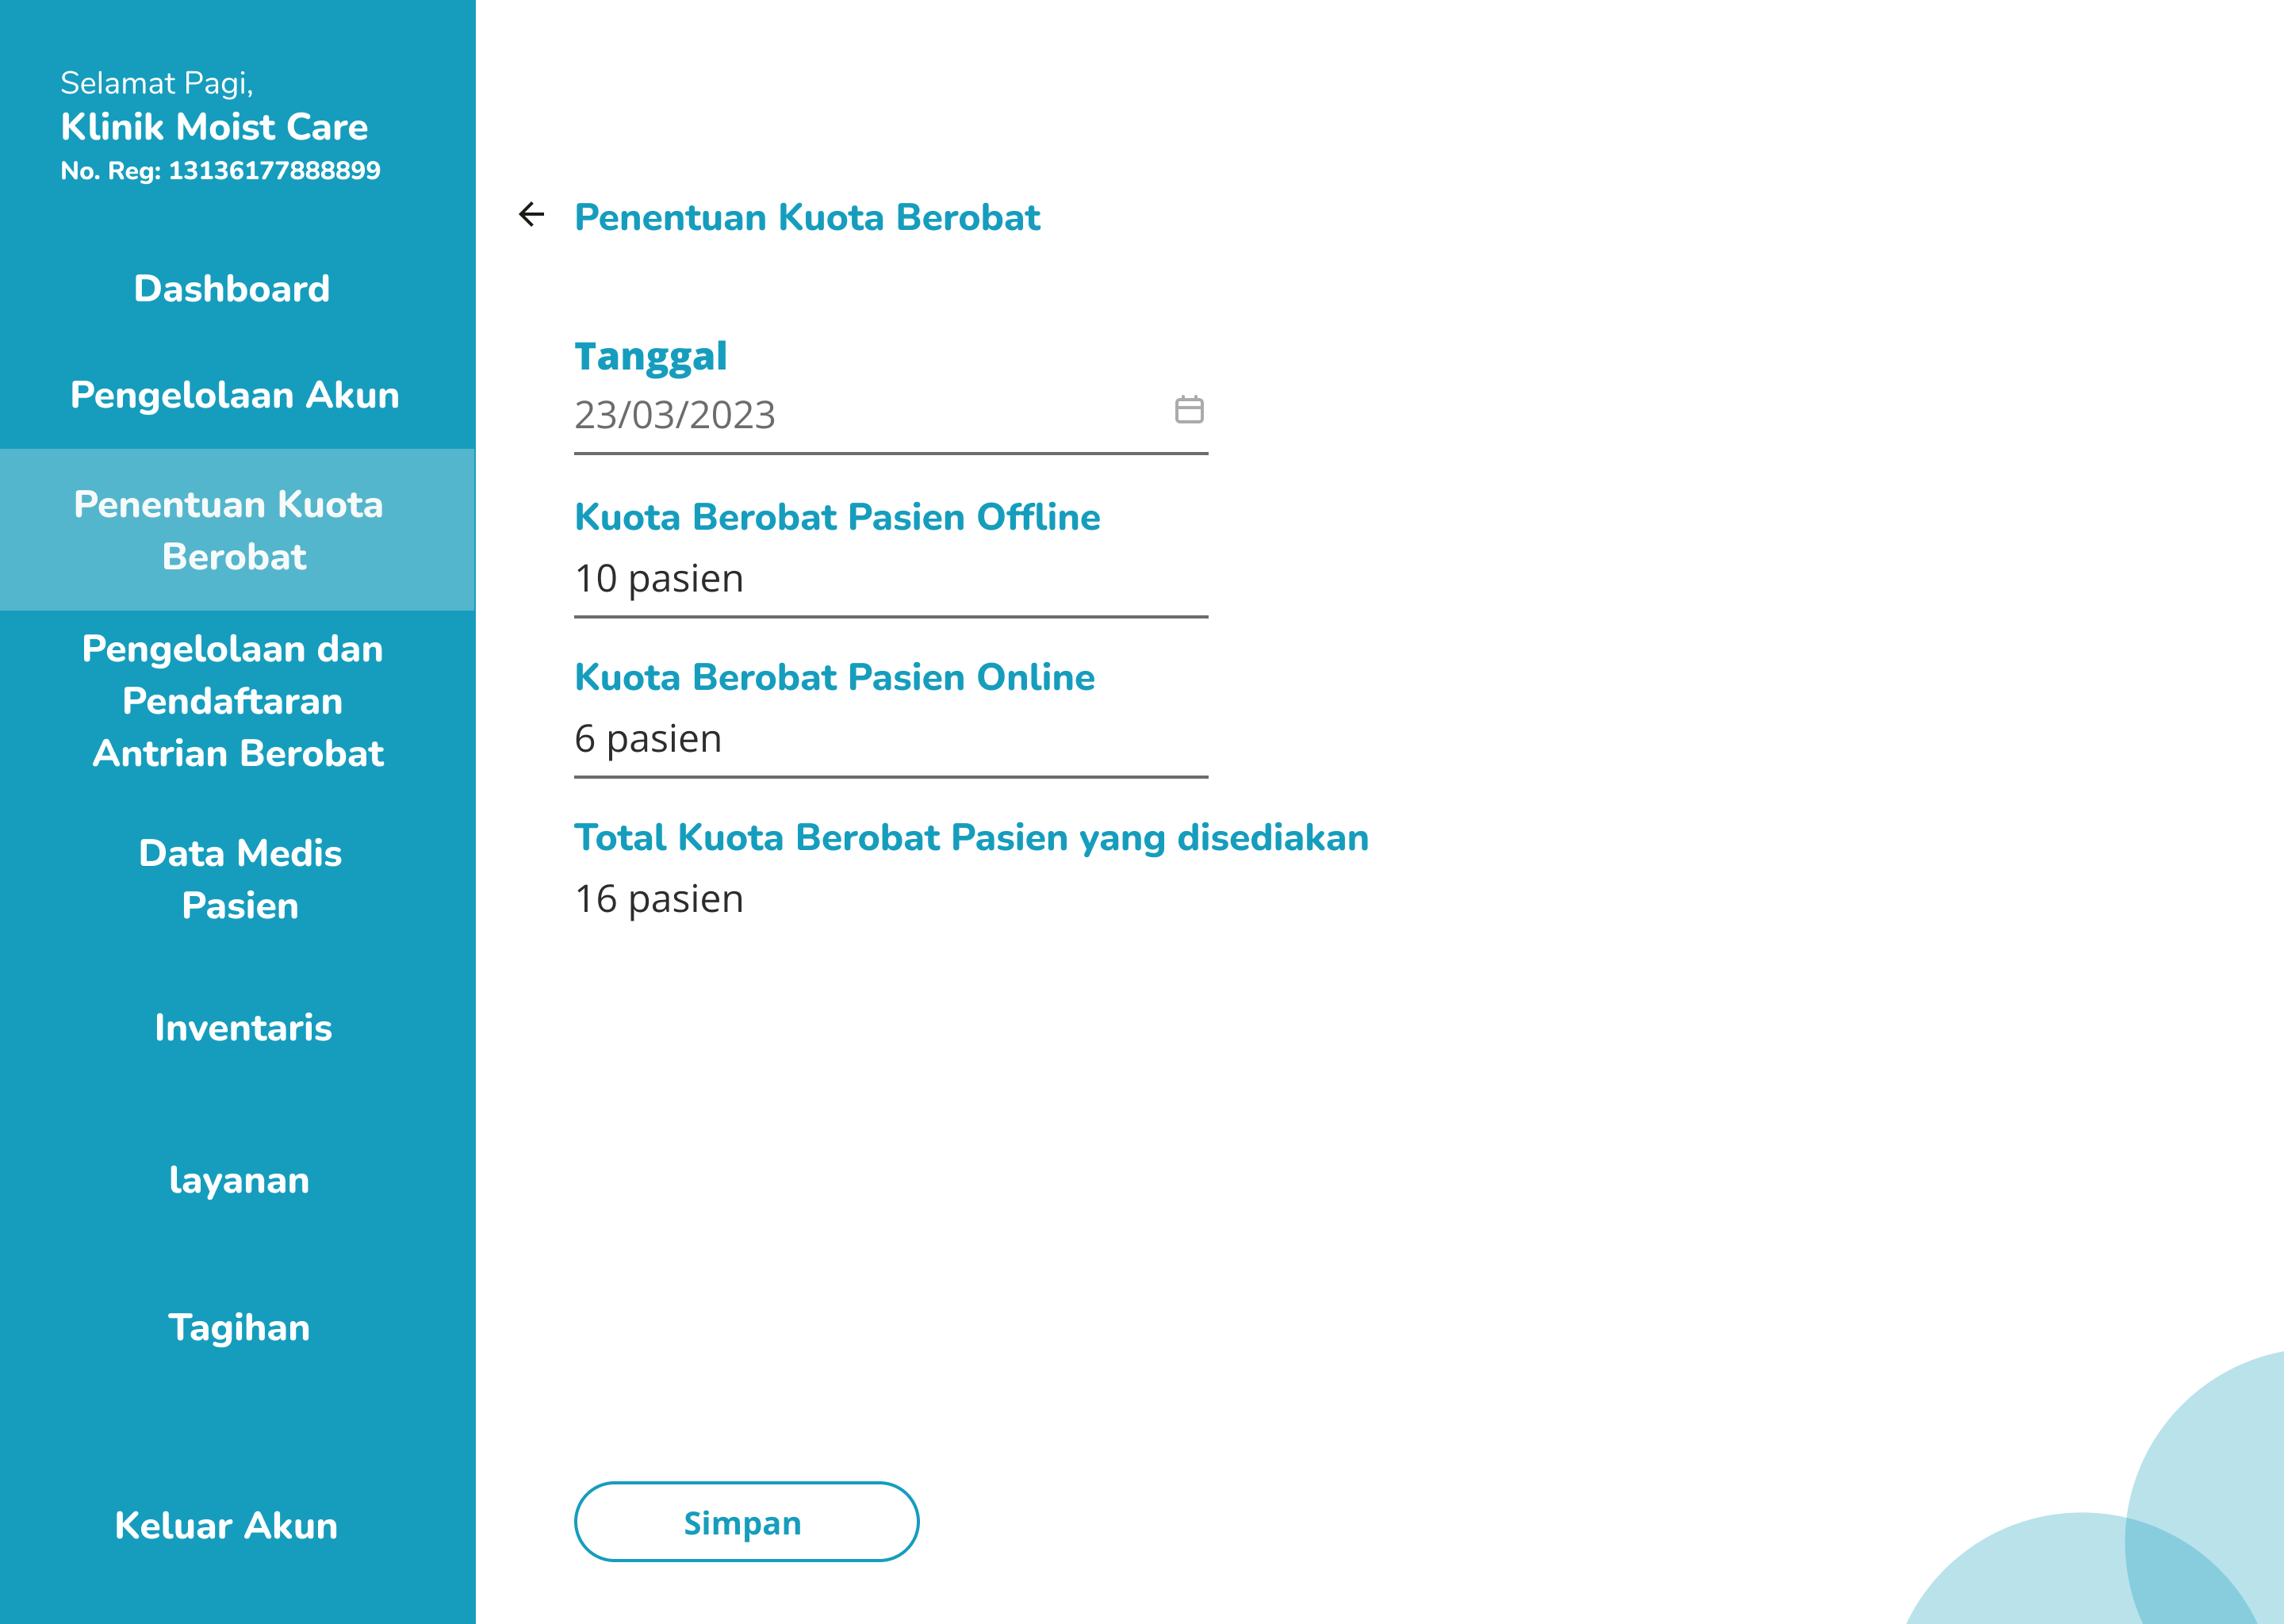
\includegraphics[width=12cm]{gambar/mockup_web/Pengelolaan Antrian Akun 1.png}
		\caption{\emph{Mock up} menentukan kuota pelayanan pasien yang mendaftar secara \emph{offline} maupun \emph{online} pada hari yang ditentukan}
		\label{Gambar:pengelolaanantrian1}
	\end{figure}
	
	Pada halaman ini admin harus memilih dan mengisi tanggal berobat beserta kuota pasien yang daftar berobat secara \emph{online} dan kuota pasien yang mendaftar secara \emph{offline} atau daftar langsung di klinik. Dan terdapat tombol simpan untuk menyimpan data kuota berobat pada hari yang ditentukan yang telah diisi.
	
	\textbf{Gambar 4.20} merupakan tampilan awal melakukan pendaftaran pasien yang akan berobat secara \emph{offline} maupun \emph{online}. Terdapat \emph{fields} memilih tanggal untuk mengambil data kuota berobat pada hari yang ditentukan yang telah di-\emph{set} sebelumnya. Lalu terdapat \emph{list} antrian pasien berobat yang sudah dikonfirmasi pendaftarannya beserta tombol ceklis untuk memvalidasi bahwa pasien sudah mendapatkan pelayanan berobat klinik dan tombol silang untuk membatalkan pasien yang sudah dikonfirmasi pendaftarannnya apabila pasien tidak jadi berobat. 
	
	\begin{figure}[H]
		\centering
		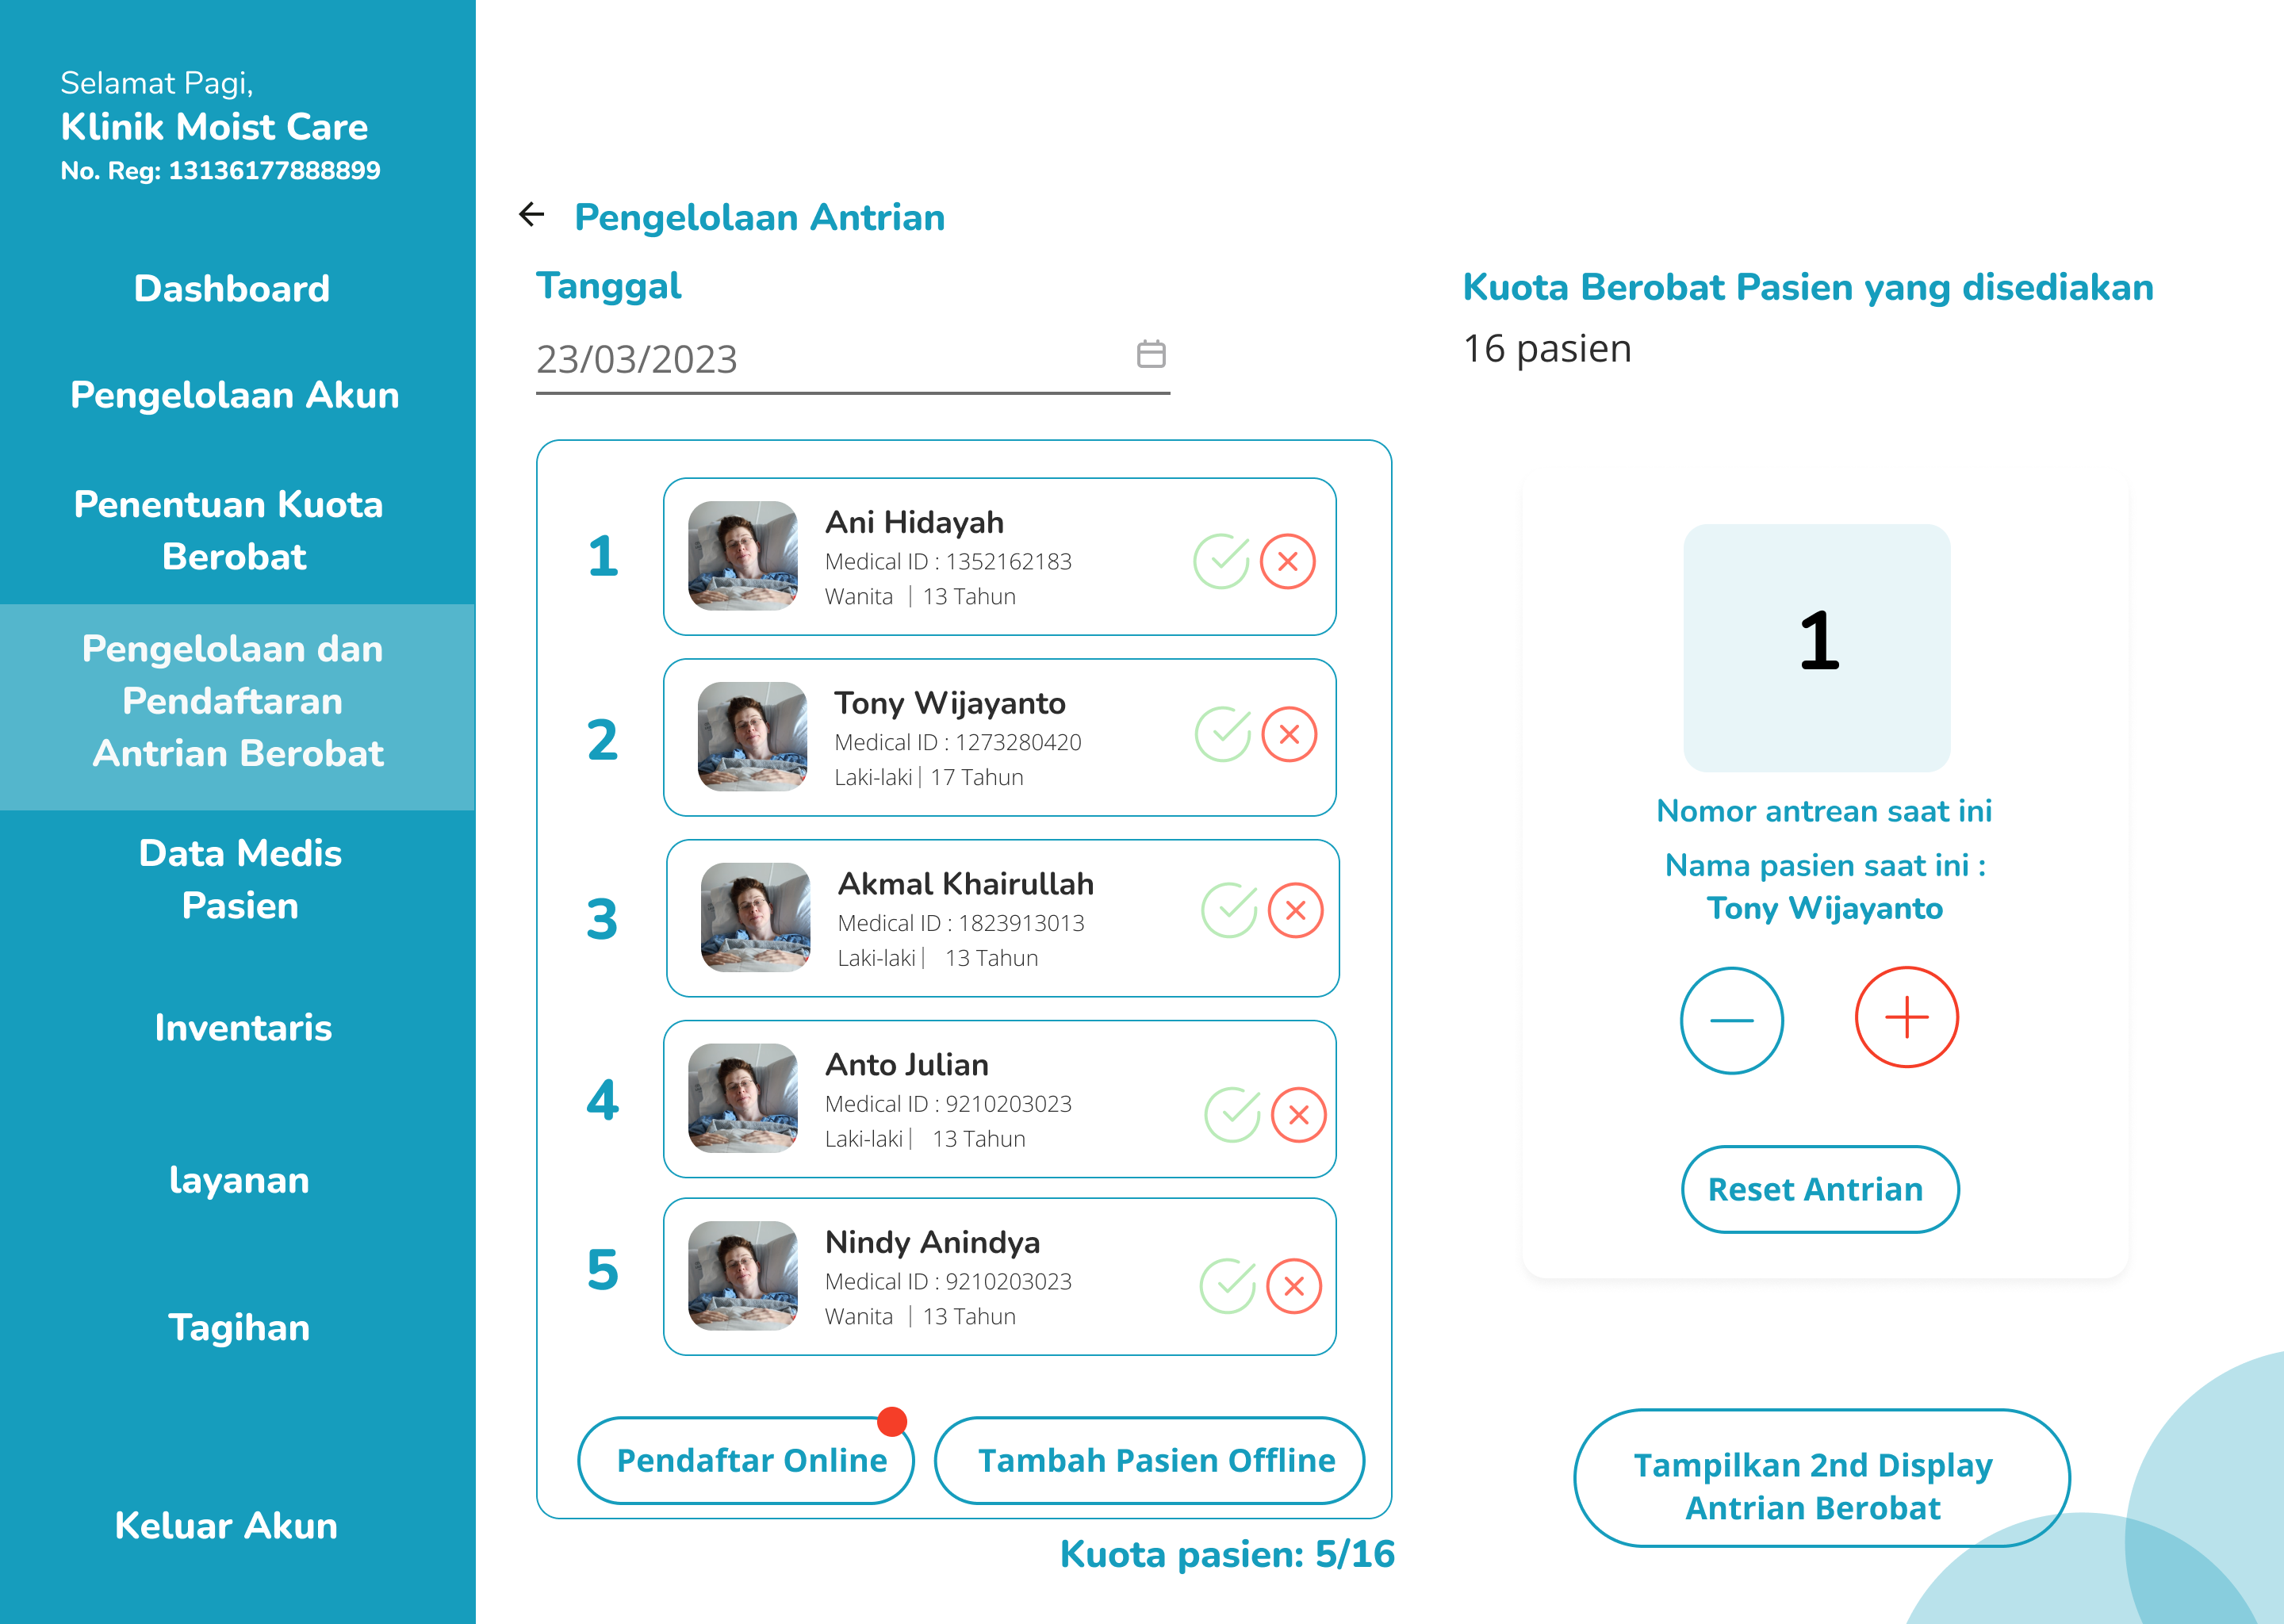
\includegraphics[width=12cm]{gambar/mockup_web/Pengelolaan Antrian Akun 2.png}
		\caption{\emph{Mock up} tampilan awal melakukan pendaftaran pasien yang akan berobat secara \emph{offline} maupun \emph{online}}
		\label{Gambar:pendaftaranakunberobat}
	\end{figure}

	Selanjutnya terdapat tombol pendaftar \emph{online} untuk melihat \emph{list} pasien yang sudah mendaftar berobat secara \emph{online} namun belum dikonfirmasi. Terdapat juga tombol tambah \emph{offline} untuk tambah pasien berobat secara manual apabila pasien daftar secara \emph{offline} atau langsung. lalu tombol \emph{plus icon} untuk memajukan antrian dan tombol \emph{minus icon} untuk memundurkan antrian. Selanjutnya tombol \emph{reset} antrian untuk me-\emph{reset} antrian kembali ke nomor 1. Dan tombol tampilkan \emph{2nd display} antrian berobat untuk tampilan tv \emph{live} di ruang tunggu pasien.
	
	Ketika admin menekan tombol tambah pasien \emph{offline} pada \textbf{Gambar 4.20} pada halaman sebelumnya maka muncul \emph{list} daftar pasien pada \textbf{Gambar 4.21} beserta tombol tambah untuk meng-\emph{input} pasien ke dalam antrian berobat dan admin bisa mencari pasien yang ingin daftar berobat dengan mencari lewat \emph{Medical} ID atau nomor BPJS. Dan ada tombol kembali untuk kembali ke tampilan \textbf{Gambar 4.15}
	
	\begin{figure}[H]
		\centering
		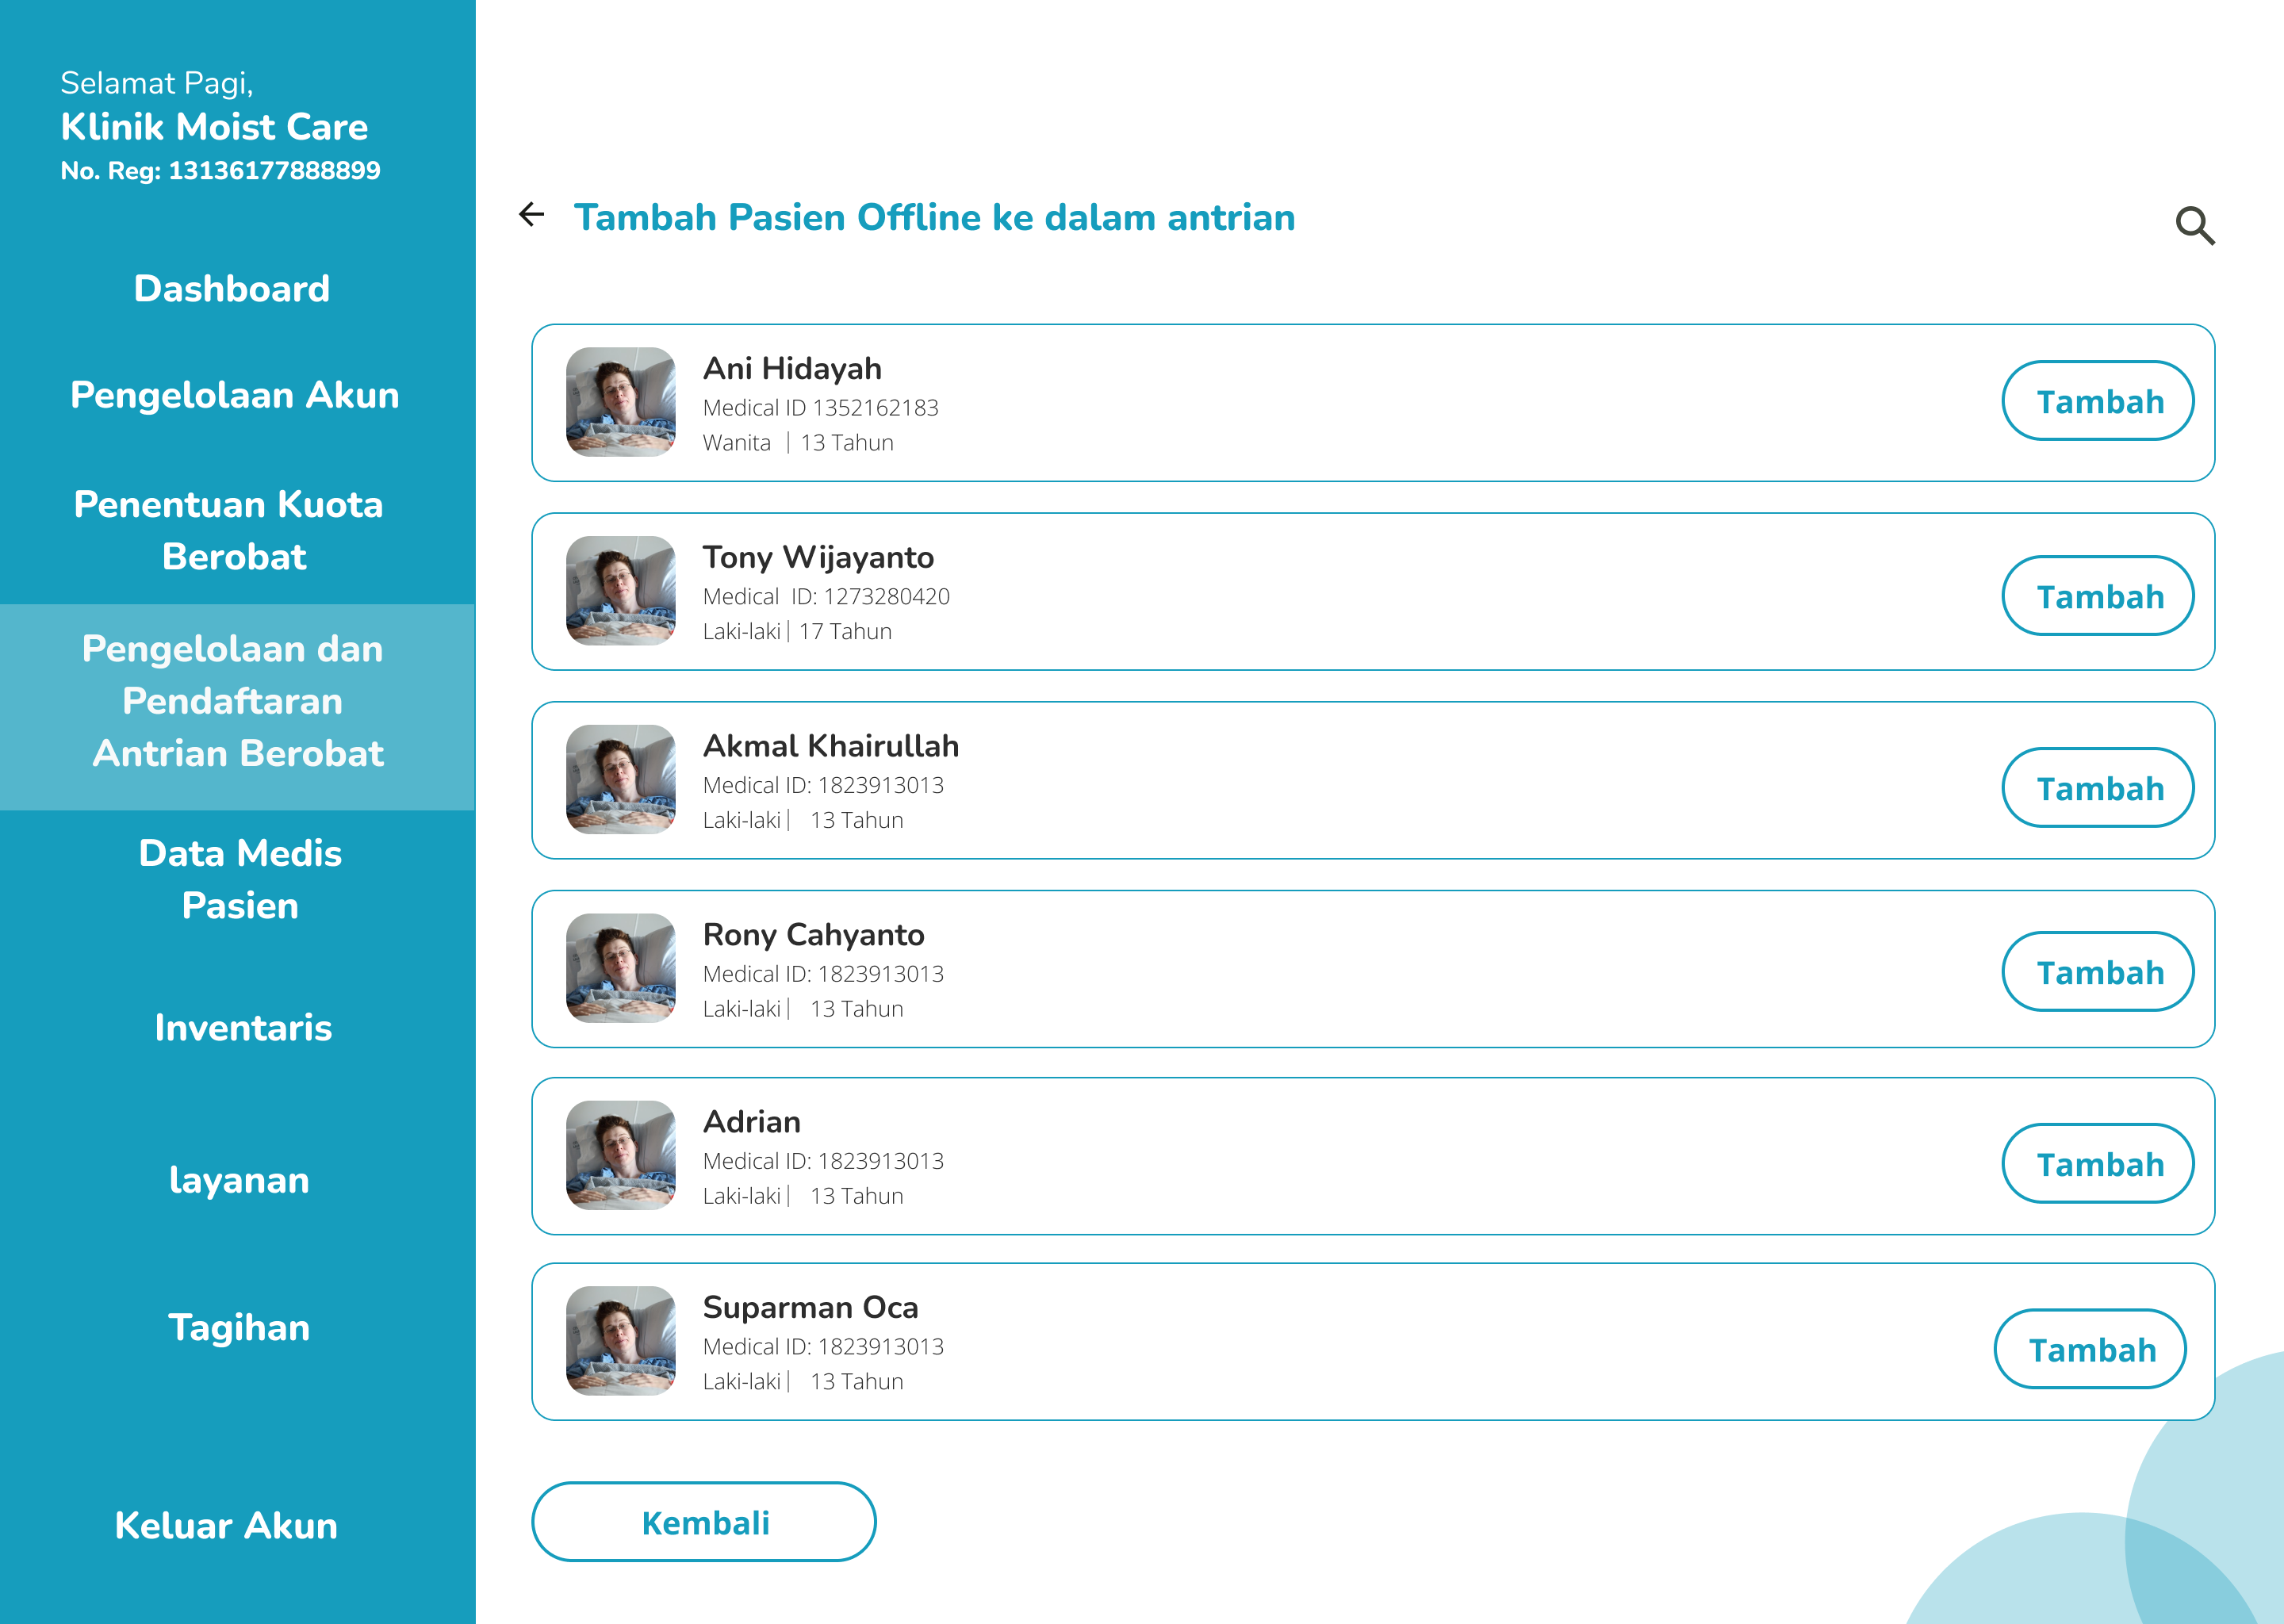
\includegraphics[width=12cm]{gambar/mockup_web/Pengelolaan Antrian Akun 3.png}
		\caption{\emph{Mock up} mendaftarkan pasien yang berobat secara \emph{offline}}
		\label{Gambar:pengelolaanantrian2}
	\end{figure}
	
	\item Desain \emph{routing table} pengelolaan antrian. 
	
	\textbf{Tabel 4.12} pada halaman selanjutnya merupakan \emph{routing table} untuk pengelolaan antrian:
	
	\begin{table}[H]
		\centering
		\caption{\emph{Routing table} pengelolaan antrian - lanjutan}
		\label{tabel_input}
		\begin{tabular}{|c|c|c|c|c|c|}
			\hline
			\textbf{\emph{Group}} & \textbf{\emph{Name}} & \textbf{API} & \textbf{HTTP} & \textbf{Keterangan} & \textbf{\emph{Return}} \\
			
			& & \textbf{\emph{Endpoint}} & \textbf{\emph{Verb}} & & \textbf{\emph{Type}} \\
			\hline
			
			Antrian & 
			\emph{CREATE} &
			/kuota &
			\emph{POST} &
			Menampilkan halaman &
			\emph{view}\\
			
			& 
			&
			&
			&
			menentukan kuota &\\
			
			& 
			&
			&
			&
			jumlah pasien berobat&\\
			\hline
			
			& 
			\emph{READ}&
			/antrian &
			\emph{GET}&
			menampilkan halaman &
			\emph{view}\\
			
			& 
			&
			&
			&
			antrian pasien berobat&\\
			\hline
			
			& 
			\emph{UPDATE}&
			/\emph{list}\_daftar&
			\emph{POST}&
			Menampilkan halaman &
			\emph{view}\\
			
			
			& 
			&
			\_berobat&
			&
			\emph{list} pasien yang telah &\\
			
			& 
			&
			\_\emph{online}&
			&
			daftar berobat \emph{online}&\\
			
			& 
			&
			&
			&
			dan dimasukkan ke &\\
			
			& 
			&
			&
			&
			dalam antrian berobat &\\
			\hline
			
			& 
			\emph{READ} &
			/\emph{list}\_daftar &
			\emph{GET} &
			Menampilkan halaman&
			\emph{view}\\
			
			& 
			&
			\_berobat&
			&
			seluruh pasien untuk&\\
			
			& 
			&
			\_\emph{offline}&
			&
			didaftarkan berobat&\\
			
			& 
			&
			&
			&
			\emph{offline} oleh klinik &\\
			
			& 
			&
			&
			&
			dan dimasukkan ke &\\
			
			& 
			&
			&
			&
			dalam antrian berobat &\\
			\hline
			
		\end{tabular}
	\end{table}

	\break
	\item Membuat \emph{database} pengelolaan antrian
	
	\begin{figure}[H]
		\centering
		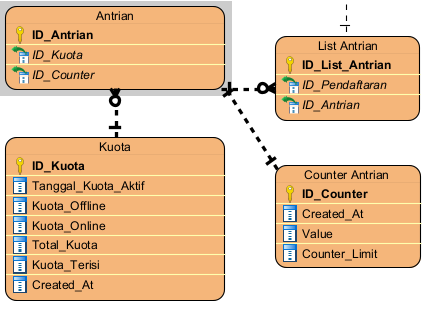
\includegraphics[width=10cm]{gambar/antrian_database.png}
		\caption{\emph{database} pengelolaan antrian}
		\label{Gambar:pengelolaanantrian2}
	\end{figure}
	
	\item Pembuatan \emph{mock up} administrasi keuangan
	
	\begin{figure}[H]
		\centering
		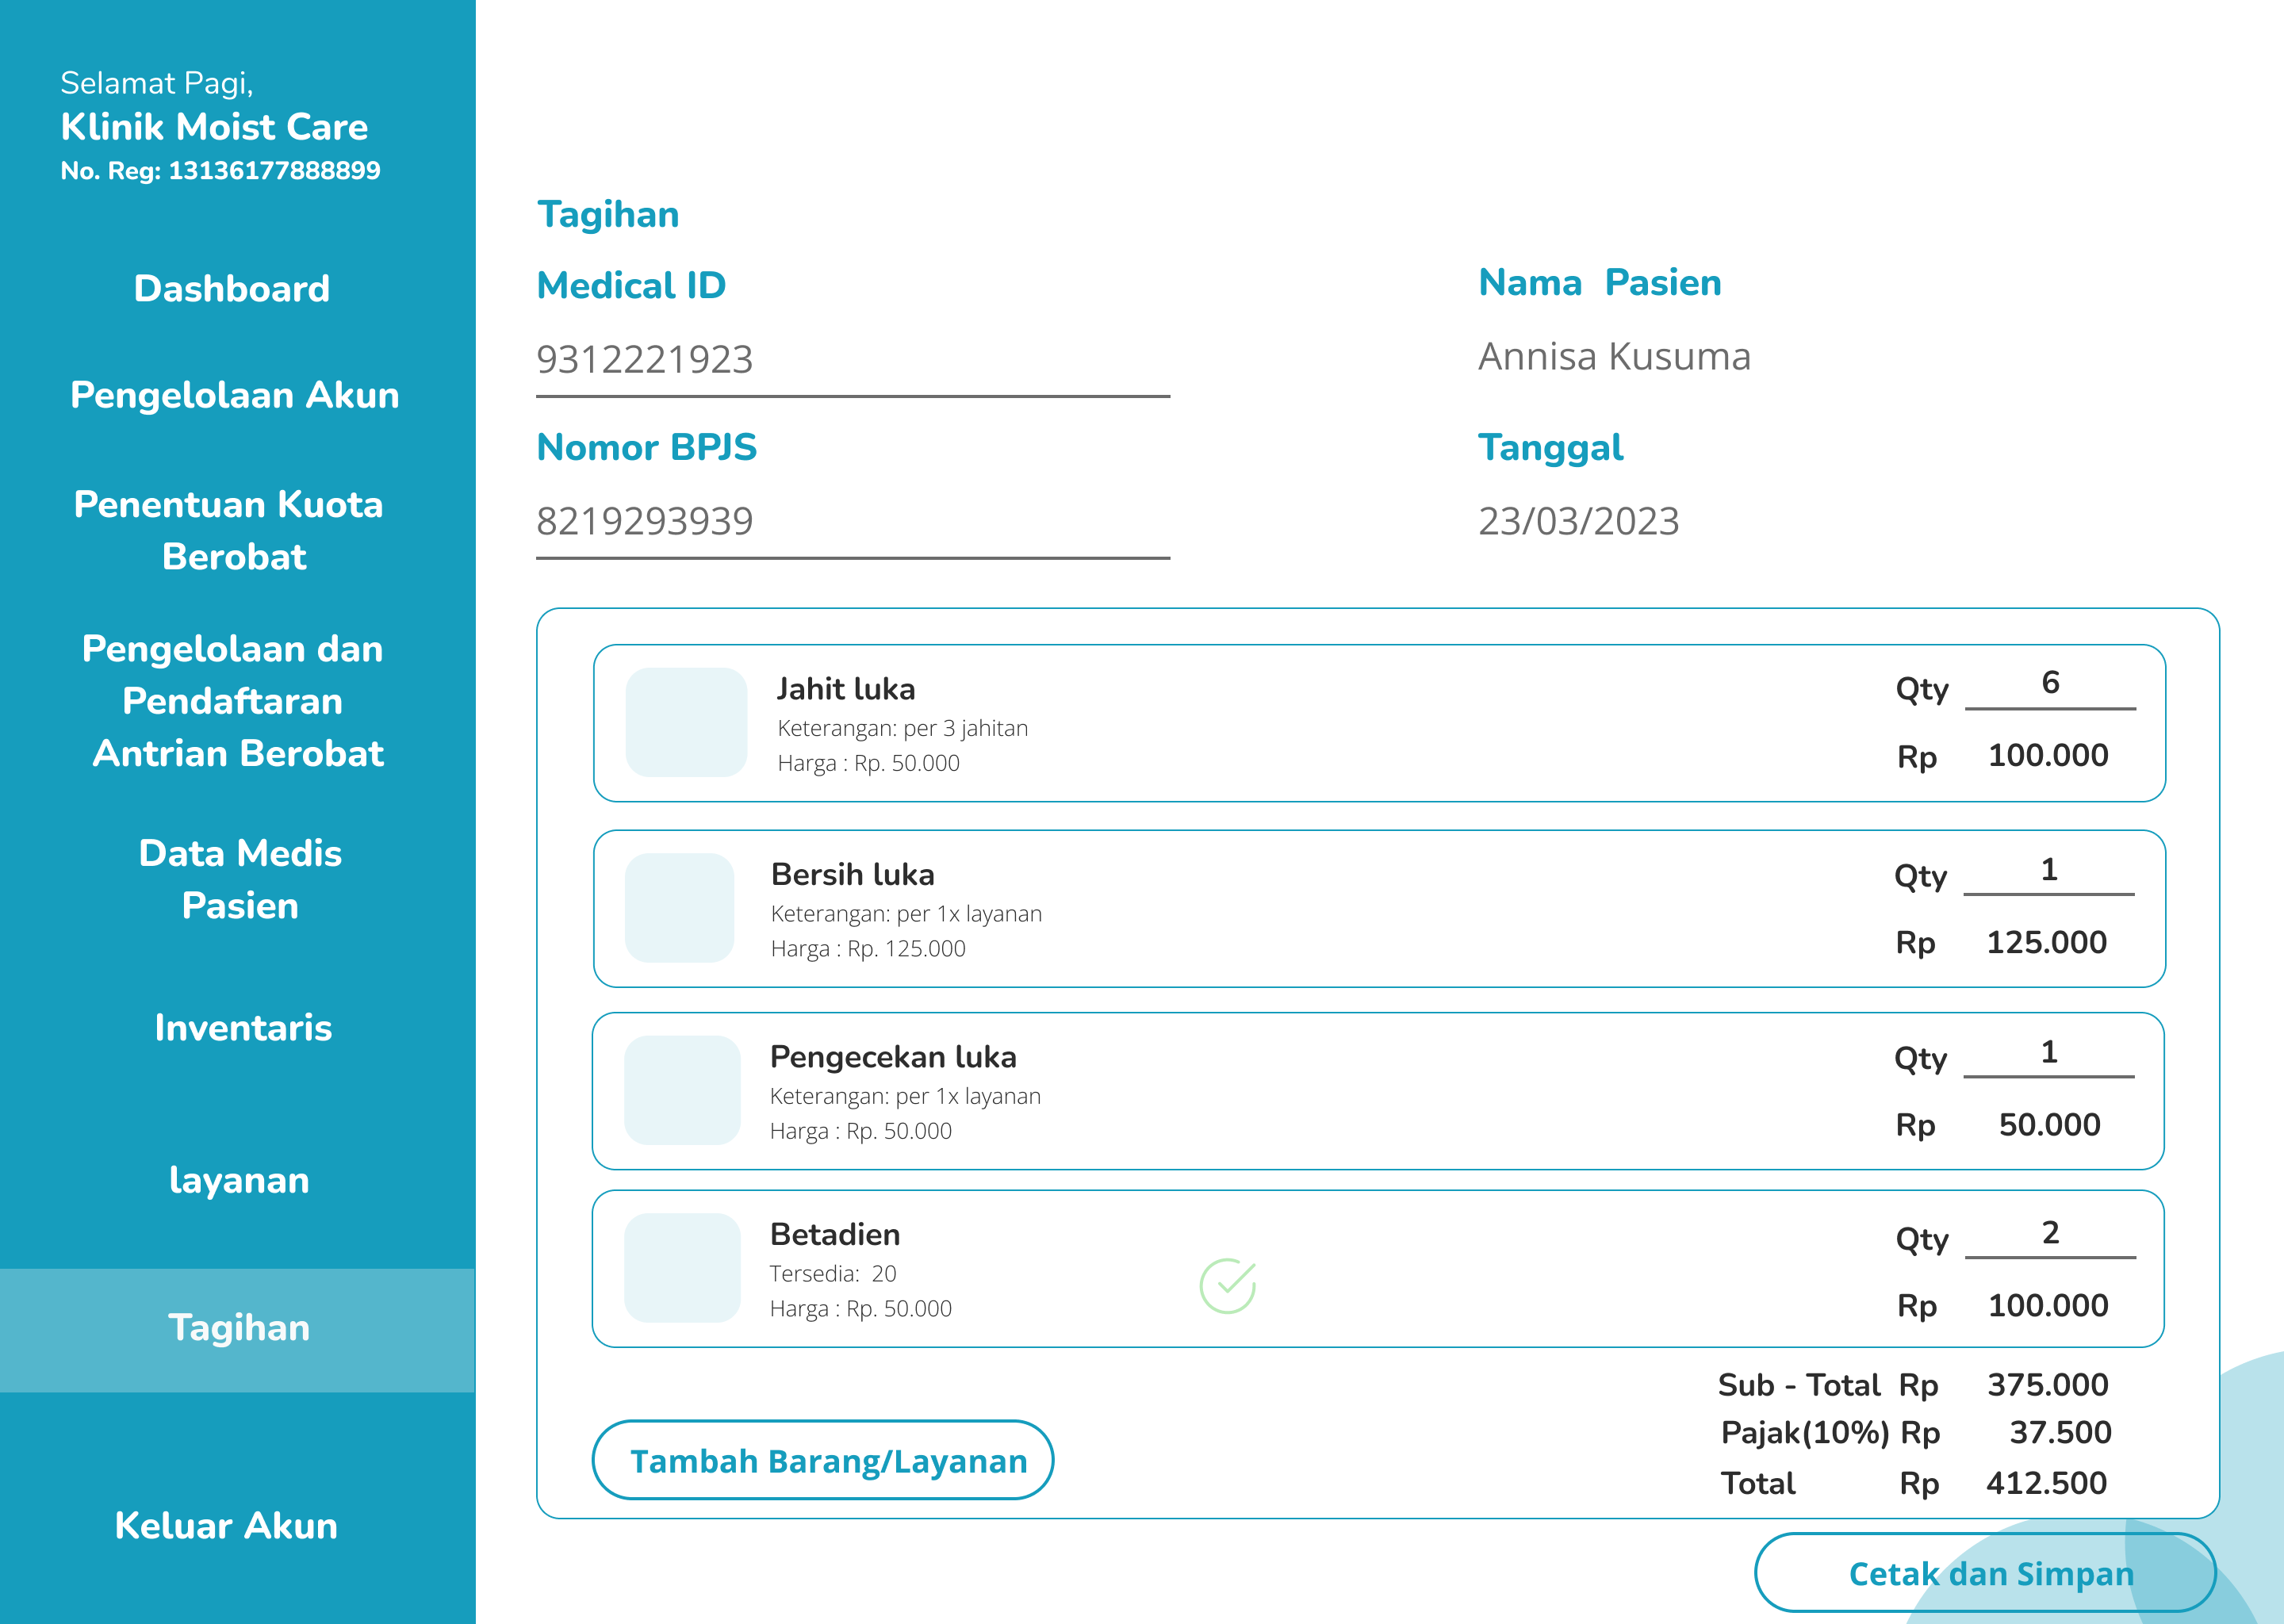
\includegraphics[width=12cm]{gambar/mockup_web/Administrasi Keuangan 1.png}
		\caption{\emph{Mock up} verifikasi dan validasi tagihan}
		\label{Gambar:pengelolaanantrian2}
	\end{figure}
	
	\textbf{Gambar 4.23} merupakan tampilan awal verifikasi dan validasi tagihan. Terdapat \emph{field Medical} ID dan Nomor BPJS untuk mencari nama pasien yang ingin membayar tagihan. Lalu ada \emph{list} barang/layanan yang digunakan pasien selama berobat beserta detail kuantitas dan harga. Di bawah \emph{list} juga terdapat keterangan harga sub-total, pajak, dan total harga dari semua barang/layanan yang digunakan pasien selama berobat. Selanjutnya terdapat cetak dan simpan untuk mencetak struk tagihan dan tombol tambah barang/layanan yang apabila admin klik akan mengarah pada \textbf{Gambar 4.21}.
	
	\textbf{Gambar 4.24} merupakan tampilan tambah barang/layanan ke dalam tagihan. Disini admin bisa mencari barang/layanan yang digunakan pasien dan menambahkannya ke dalam tagihan secara manual. Dan terdapat tombol kembali untuk kembali ke \textbf{Gambar 4.23}.
	
	\begin{figure}[H]
		\centering
		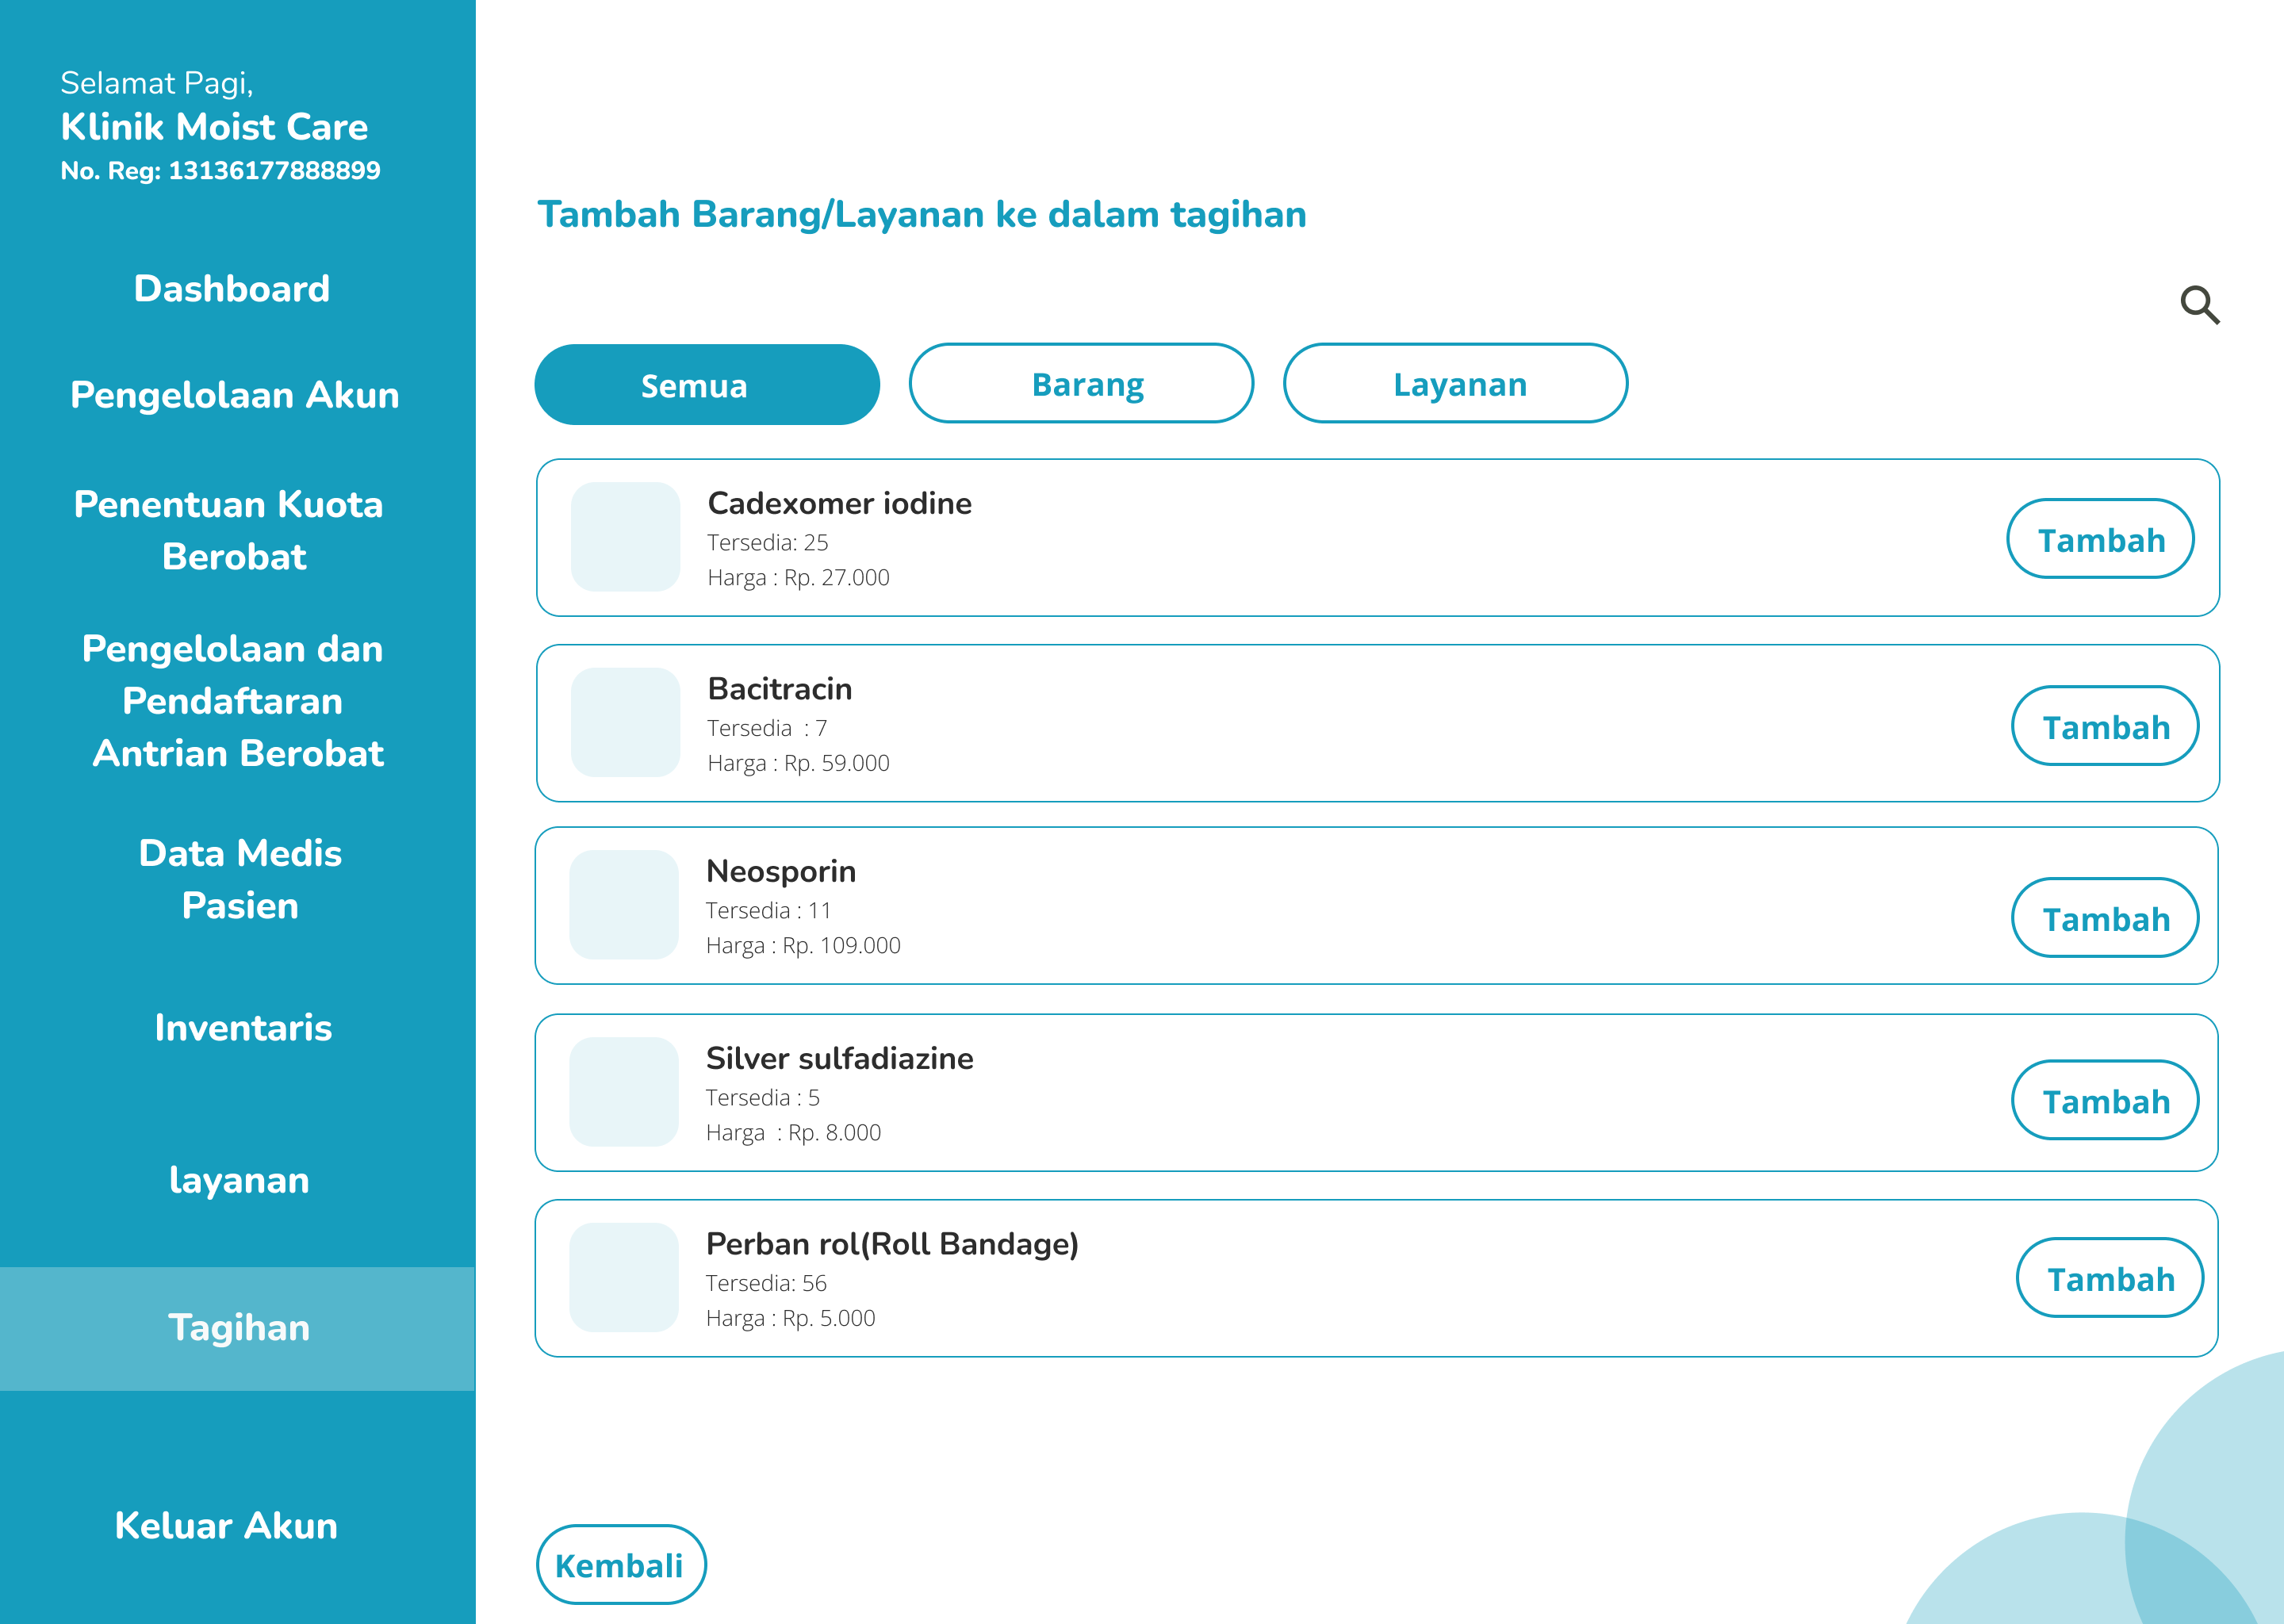
\includegraphics[width=12cm]{gambar/mockup_web/Administrasi Keuangan 2.png}
		\caption{\emph{Mock up} tambah barang/layanan pada verifikasi dan validasi tagihan}
		\label{Gambar:pengelolaanantrian2}
	\end{figure}
	
	\item Desain \emph{routing table} administrasi keuangan
	
	\textbf{Tabel 4.13} pada halaman selanjutnya merupakan \emph{routing table} untuk administrasi keuangan:
	
	\begin{table}[H]
		\centering
		\caption{\emph{Routing table} administrasi keuangan}
		\label{tabel_input}
		\begin{tabular}{|c|c|c|c|c|c|}
			\hline
			\textbf{\emph{Group}} & \textbf{\emph{Name}} & \textbf{API} & \textbf{HTTP} & \textbf{Keterangan} & \textbf{\emph{Return}} \\
			
			& & \textbf{\emph{Endpoint}} & \textbf{\emph{Verb}} & & \textbf{\emph{Type}} \\
			\hline
			
			Tagihan& 
			\emph{CREATE} &
			/tagihan&
			\emph{POST} &
			Menampilkan halaman &
			\emph{view}\\
			
			& 
			&
			&
			&
			membuat tagihan &
			\\
			\hline
			
			& 
			\emph{READ} &
			/\emph{list}\_&
			\emph{GET }&
			Menampilkan halaman &
			\emph{view}\\
			
			& 
			&
			\_tagihan&
			&
			\emph{list} semua&
			\\
			
			& 
			&
			&
			&
			tagihan yang&
			\\
			
			& 
			&
			&
			&
			pernah dibuat&
			\\
			\hline
			
		\end{tabular}
	\end{table}
	
	\item Membuat \emph{database} administrasi keuangan
	
	\begin{figure}[H]
		\centering
		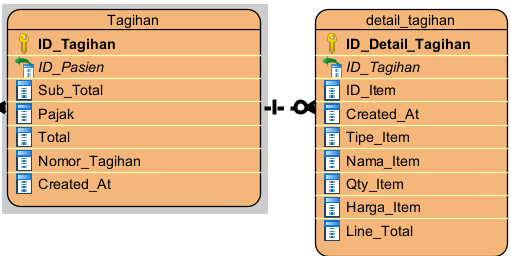
\includegraphics[width=10cm]{gambar/tagihan_database.png}
		\caption{Tabel tagihan dan tabel detail tagihan} 
		\label{Gambar:usecaseadminjurnalpertama}
	\end{figure}
	
	\textbf{Gambar 4.25} merupakan \emph{database} administrasi memiliki 2 tabel yang saling terhubung, yaitu tabel tagihan dan tabel detail tagihan. Tabel tagihan memuat beberapa atribut yaitu id\_tagihan, id\_pasien, sub\_total, pajak, total, nomor\_tagihan, dan \emph{created\_at}. Tabel detail tagihan memuat beberapa atribut yaitu id\_detail\_tagihan, id\_tagihan, id\_\emph{item}, tipe\_\emph{item}, nama\_\emph{item}, qty\_\emph{item}, harga\_\emph{item}, \emph{line\_total} dan \emph{created\_at}. Data tersebut akan disimpan pada \emph{database} MongoDB dan disimpan dalam format JSON.
	
	\break
	\item Rancangan \emph{use case} diagram
	
	\begin{figure}[H]
		\centering
		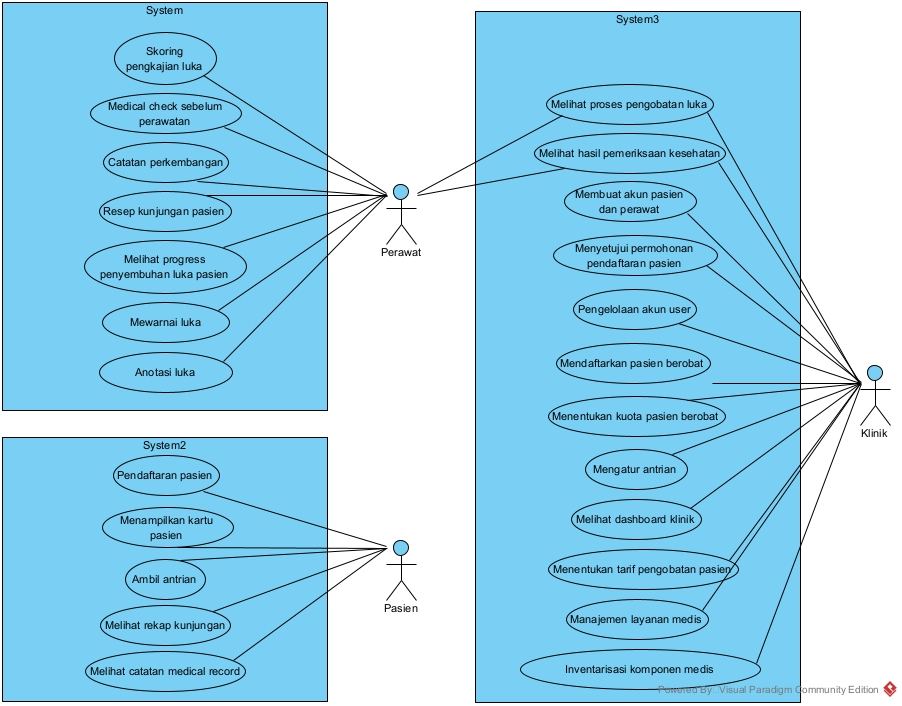
\includegraphics[width=14cm]{diagram/Use Case Diagram WCare Fix.jpg}
		\caption{\emph{Use case} diagram} 
		\label{Gambar:usecaseadminjurnalpertama}
	\end{figure}
	
	%\break
	%\item Rancangan desain \emph{class} diagram
	
	%\begin{figure}[H]
	%	\centering
	%	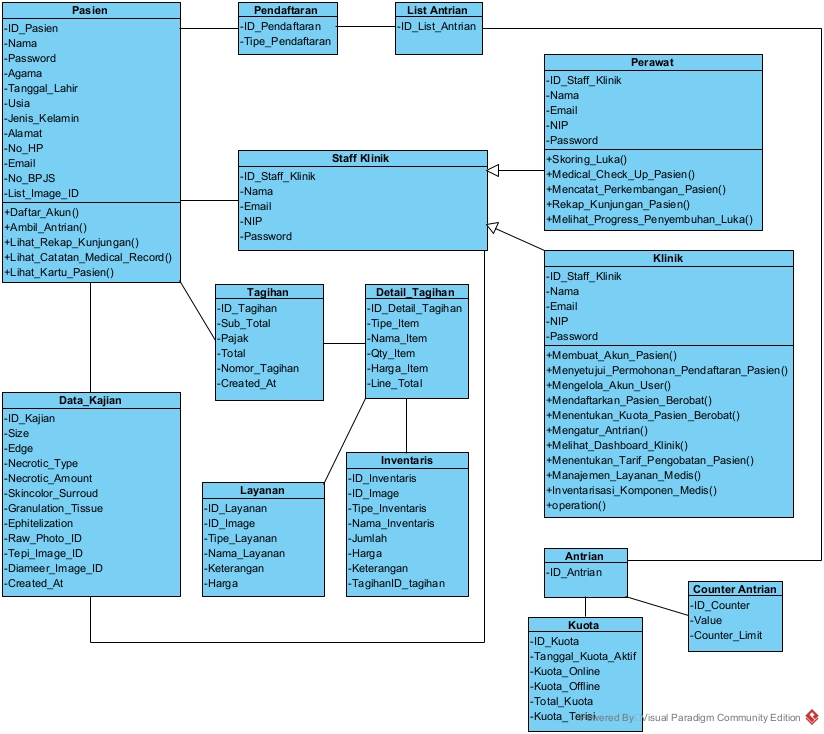
\includegraphics[width=14cm]{diagram/Class Diagram WCare Rev.jpg}
	%	\caption{\emph{class} diagram} 
	%	\label{Gambar:usecaseadminjurnalpertama}
	%\end{figure}
	
	\break
	\item Rancangan desain \emph{database} sistem
	
	\begin{figure}[H]
		\centering
		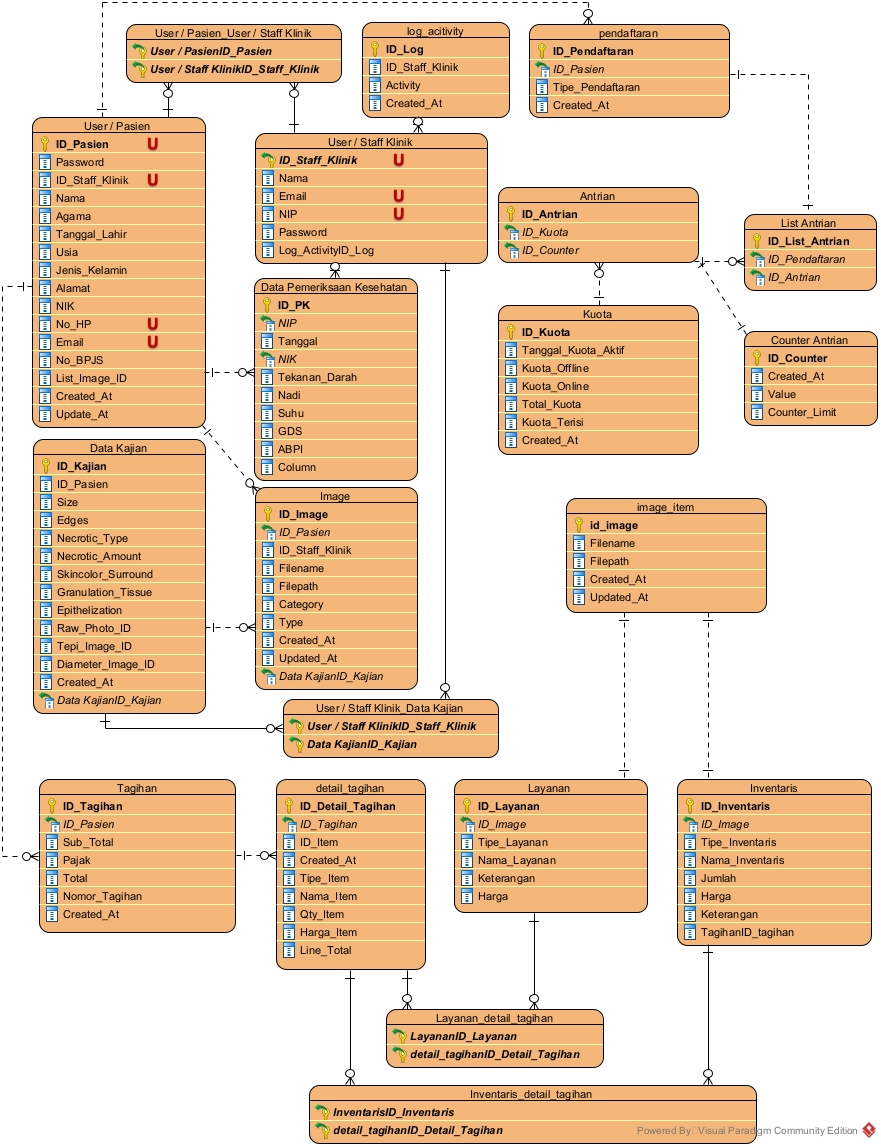
\includegraphics[width=14cm]{diagram/WCare Webapp Rev Fix.jpg}
		\caption{Desain \emph{database} sistem} 
		\label{Gambar:usecaseadminjurnalpertama}
	\end{figure}
	
\end{enumerate}

\subsection{\emph{Sprint}-2}
\begin{table}[H]
	\centering
	\caption{\emph{Sprint}-2 \emph{backlog}}
	\label{tabel_input}
	\begin{tabular}{|c|l|l|l|}
		\hline
		\textbf{No} & \textbf{\emph{User Story}} & \textbf{\emph{Task}} & \textbf{Status} \\
		\hline
		
		1 & 
		\emph{Dashboard klinik} & 
		1. implementasi \emph{view login} perawat &
		selesai\\
		
		& 
		& 
		/admin &
		\\
		
		& 
		& 
		2. implementasi \emph{web service login} &
		\\
		
		& 
		& 
		perawat/admin klinik.&
		\\
		
		& 
		& 
		3. implementasi \emph{dashboard} klinik.&
		\\
		\hline
		
		2 & 
		Pembuatan akun & 
		1. implementasi \emph{web service login} &
		selesai\\
		
		& 
		pasien& 
		pasien&
		\\
		
		& 
		& 
		2. implementasi \emph{view} registrasi
		&
		\\
		
		& 
		& 
		pasien dari klinik.&
		\\
		
		
		& 
		& 
		3. implementasi \emph{web service} registrasi &
		\\
		
		& 
		& 
		pasien &
		\\
		
		
		& 
		& 
		4. implementasi \emph{view list} permohonan &
		\\
		
		& 
		& 
		akun pasien.&
		\\
		
		& 
		& 
		5. implementasi \emph{web service list}&
		\\
		 
		& 
		& 
		permohonan akun pasien.&
		\\
		
		& 
		& 
		6. implementasi \emph{view list} pasien&
		\\
		
		& 
		& 
		terdaftar klinik.&
		\\
		
		& 
		& 
		7. implementasi \emph{web service list} &
		\\
		
		& 
		& 
		pasien terdaftar klinik.&\\
		\hline
		
	\end{tabular}
\end{table}

\begin{enumerate}
	
	\item Implementasi \emph{view} login admin/perawat
	
	Berikut merupakan implementasi \emph{view} login admin/perawat menggunakan \emph{Visual Studio Code}. \emph{Code}-nya ada pada lampiran E dan menghasilkan tampilan \emph{view} seperti pada \textbf{Gambar 4.28}.
	
	\begin{figure}[H]
		\centering
		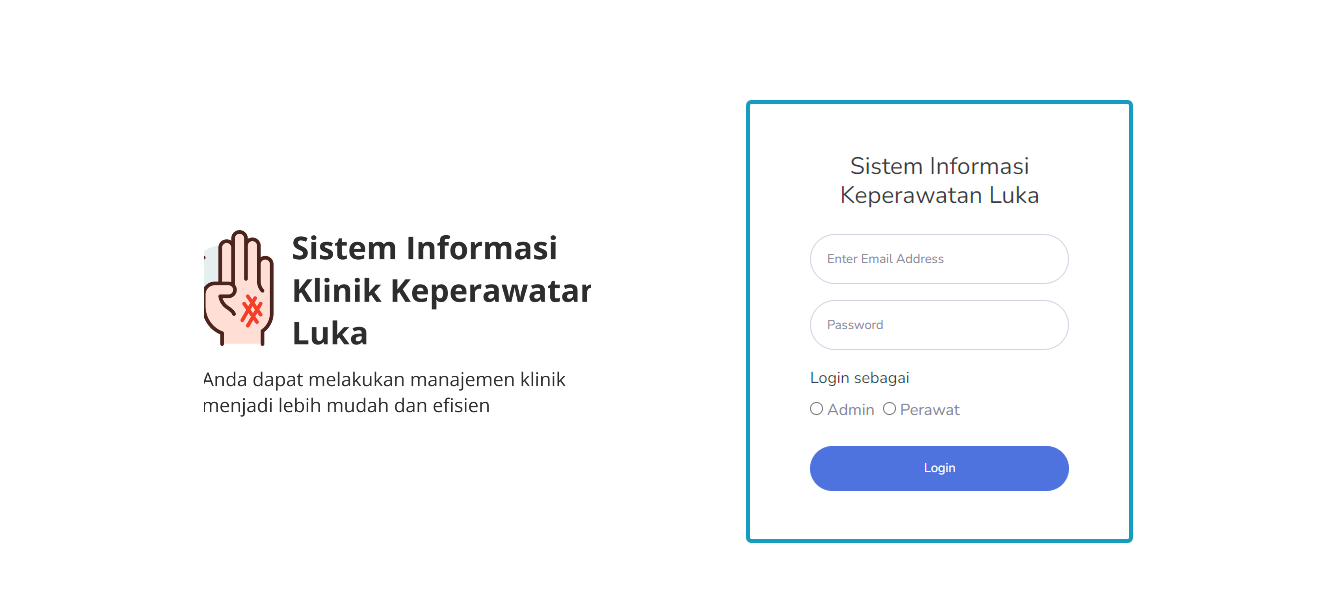
\includegraphics[width=14cm]{gambar/login_view.png}
		\caption{Realisasi \emph{view login} admin/perawat} 
		\label{Gambar:usecaseadminjurnalpertama}
	\end{figure}
	
	\item Implementasi \emph{web service login} perawat/admin klinik
	
	\emph{Web service} dibuat menggunakan framework \emph{flask}. \emph{flask} adalah \emph{web service} berbasis \emph{python}. URL \emph{Routing} untuk melakukan \emph{login} akun admin/perawat adalah jft.web.id/woundapiv2/login\_apps.
	
	\emph{Code} untuk \emph{web service login} admin/perawat ada pada lampiran F, metode yang digunakan adalah \emph{POST}. Pada saat pemanggilan \emph{web service}, terlebih dulu dilakukan pengecekan apakah sudah ada data yang sama berdasarkan email, \emph{password} dan \emph{role} atau belum, jika sudah ada maka akan dikembalikan ke halaman \emph{view home} berisi halaman \emph{dashboard} yang menandakan berhasil \emph{login}, jika data tidak tersedia maka akan dikembalikan ke halaman \emph{view login} yang menandakan bahwa \emph{user} tidak ditemukan.
	
	\item Implementasi \emph{dashboard} klinik
	
	Berikut merupakan implementasi \emph{dashboard} klinik. \emph{Code}-nya ada pada lampiran G dan menghasilkan tampilan \emph{view} seperti pada \textbf{Gambar 4.29}. Namun belum berjalan semestinya dan data yang ditampilkan hanya data statis dan masih bersifat \emph{dummy}.
	
	\begin{figure}[H]
	\centering
	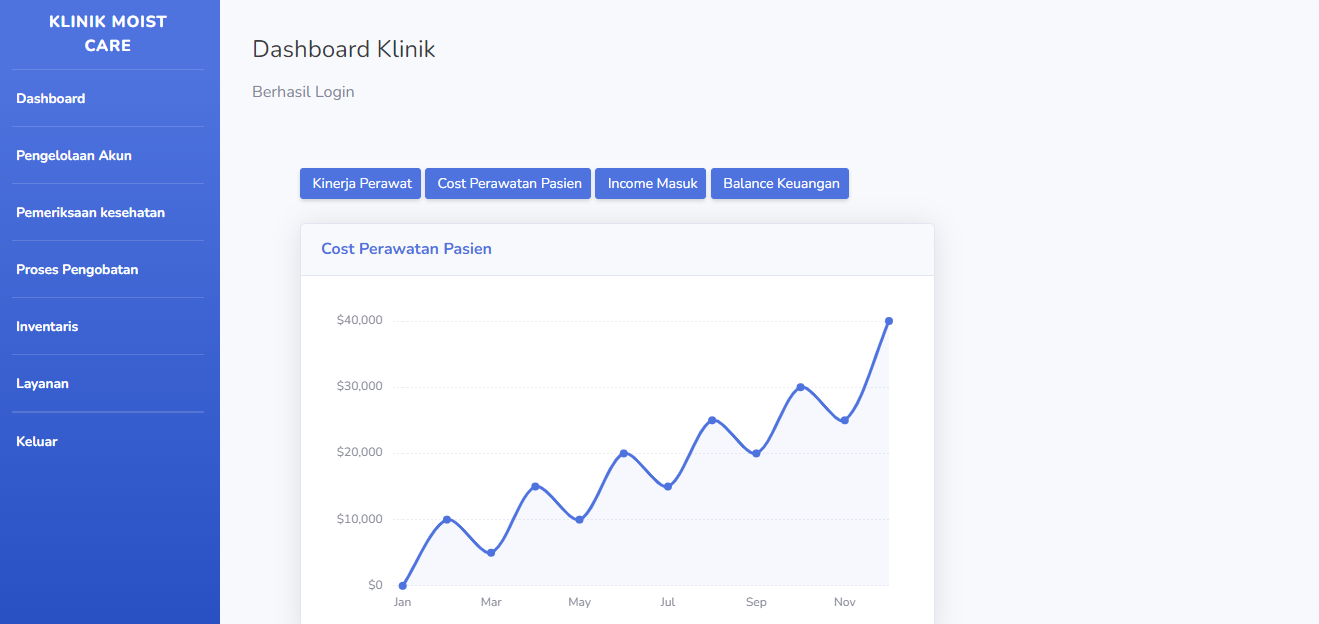
\includegraphics[width=14cm]{gambar/dashboard_view.png}
	\caption{Realisasi \emph{view dashboard} klinik} 
	\label{Gambar:usecaseadminjurnalpertama}
	\end{figure}
	
	\item Implementasi \emph{web service} login pasien
	
	URL \emph{Routing} yang digunakan untuk melakukan \emph{login} akun pasien adalah jft.web.id/woundapiv2/login\_pasien.
	
	\emph{Code} untuk \emph{web service login} pasien ada pada lampiran H, metode yang digunakan adalah \emph{POST}. Pada saat pemanggilan \emph{web service}, terlebih dulu dilakukan pengecekan apakah sudah ada data yang sama berdasarkan email, \emph{password} dan status verifikasi pasien atau belum, jika sudah ada maka akan dikembalikan ke pesan \emph{success} dengan status HTTP 200, jika data tidak sesuai maka akan dikembalikan ke pesan \emph{failed} dengan status HTTP 400. \textbf{Gambar 4.30} pada halaman selanjutnya merupakan pengecekan \emph{web service login} pasien yang sudah dapat digunakan dan dilakukan menggunakan POSTMAN.
	
	\begin{figure}[H]
	\centering
	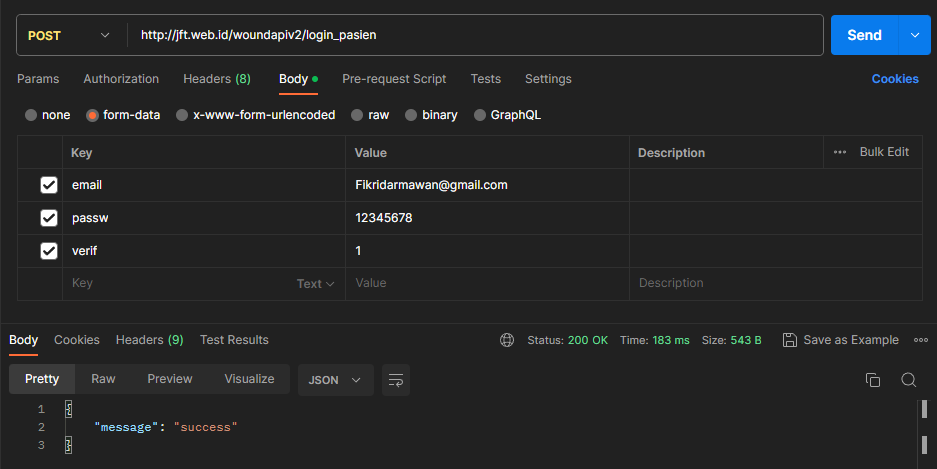
\includegraphics[width=14cm]{gambar/webservice_login_pasien.png}
	\caption{Pemanggilan \emph{web service} login pasien} 
	\label{Gambar:usecaseadminjurnalpertama}
	\end{figure}
	
	\item Implementasi \emph{view} registrasi pasien dari klinik
	
	Berikut merupakan implementasi \emph{view} registrasi pasien dari klinik. \emph{Code}-nya ada pada lampiran I dan menghasilkan tampilan \emph{view} seperti pada \textbf{Gambar 4.31}.
	
	\begin{figure}[H]
		\centering
		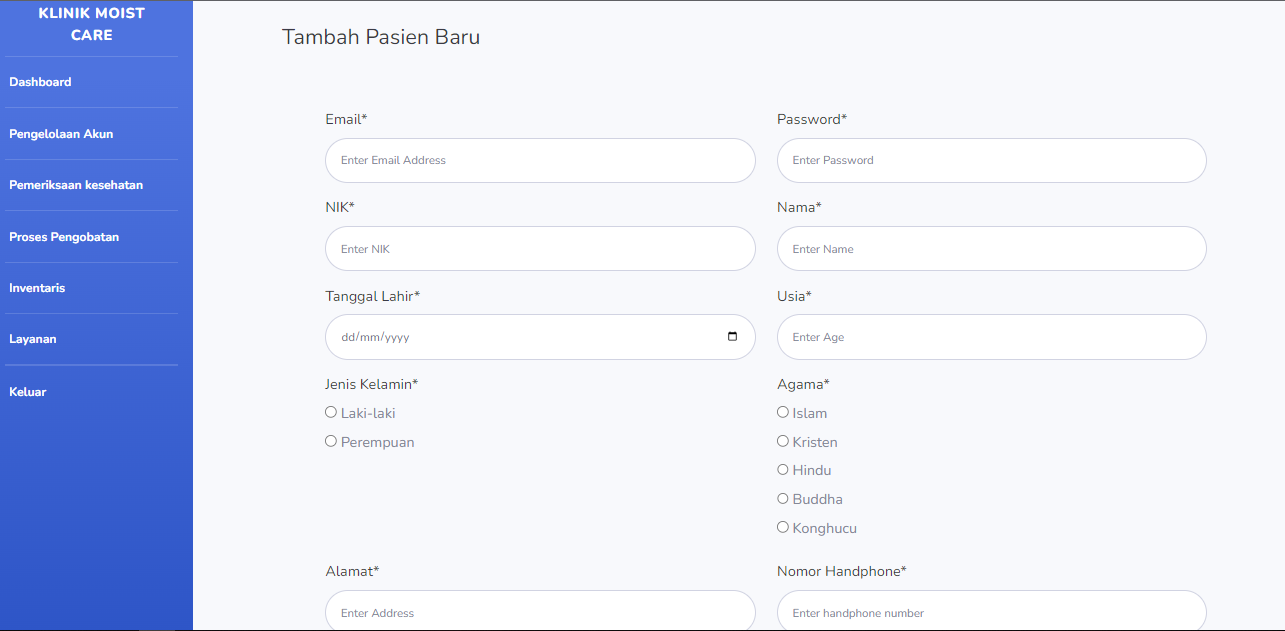
\includegraphics[width=14cm]{gambar/tambah_pasien_view.png}
		\caption{Realisasi \emph{view} registrasi pasien dari klinik} 
		\label{Gambar:usecaseadminjurnalpertama}
	\end{figure}
	
	\break
	\item Implementasi \emph{web service} registrasi pasien dari klinik
	
	URL \emph{Routing} yang digunakan untuk melakukan registrasi akun pasien dari klinik adalah jft.web.id/woundapiv2/add\_new\_patient.
	
	\emph{Code} untuk \emph{web service} registrasi akun pasien ada pada lampiran J, metode yang digunakan adalah \emph{POST}. Pada saat pemanggilan \emph{web service}, admin terlebih dulu mengisi data email, \emph{password}, NIK, nama, jenis kelamin, agama, tanggal lahir, usia, alamat, nomor HP lalu dilakukan pengecekan apakah sudah ada data yang sama atau belum, jika sudah ada maka akan dikembalikan ke halaman \emph{view} registrasi pasien beserta pesan "gagal \emph{input} pasien", jika data belum tersedia maka akan dikembalikan ke halaman \emph{view} registrasi pasien beserta pesan "berhasil \emph{input} pasien".
	
	\item Implementasi \emph{view list} permohonan akun pasien
	
	Berikut merupakan implementasi \emph{view list} permohonan akun pasien dari klinik. \emph{Code}-nya ada pada lampiran K dan menghasilkan tampilan \emph{view} seperti pada \textbf{Gambar 4.32}.
	
	\begin{figure}[H]
		\centering
		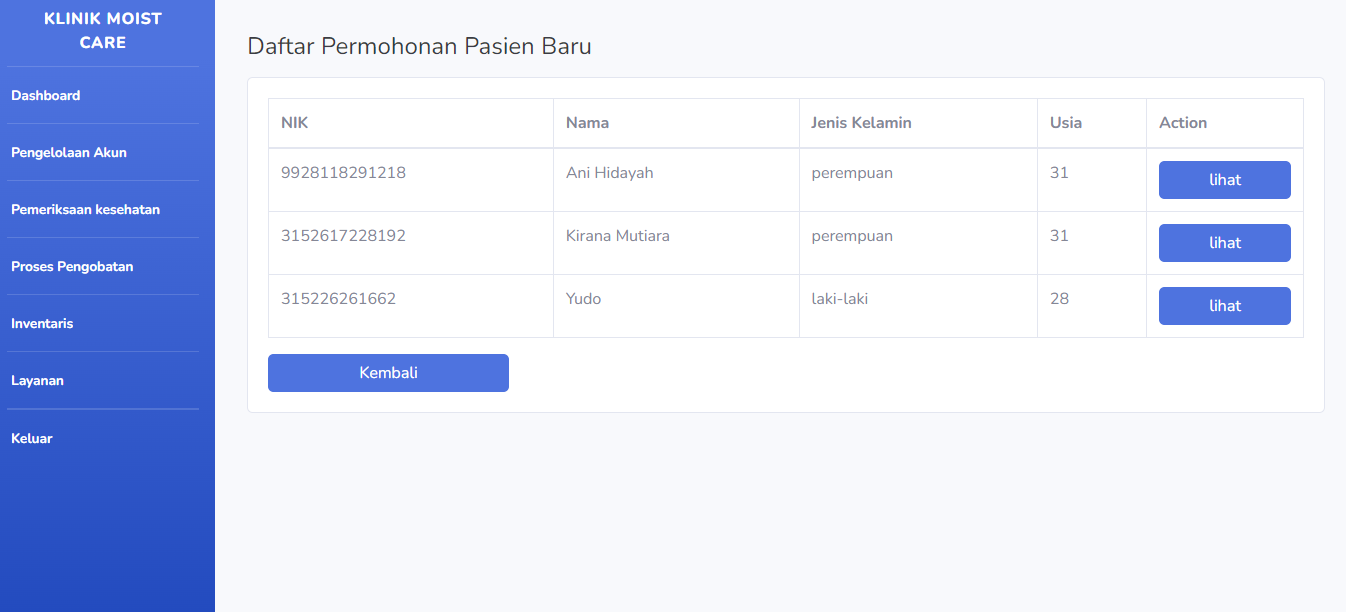
\includegraphics[width=14cm]{gambar/daftar_pemohon_pasien_view.png}
		\caption{Realisasi \emph{view list} permohonan akun pasien} 
		\label{Gambar:usecaseadminjurnalpertama}
	\end{figure}
	
	\break
	\item Implementasi \emph{web service list} permohonan akun pasien
	
	URL \emph{Routing} yang digunakan untuk \emph{list} permohonan akun pasien untuk diverifikasi klinik adalah jft.web.id/woundapiv2/list\_request\_new\_patient.
	
	\emph{Code} untuk \emph{web service} \emph{list} permohonan akun pasien untuk diverifikasi klinik ada pada lampiran L, metode yang digunakan adalah \emph{GET}. Pada saat pemanggilan \emph{web service} data berupa nama, jenis kelamin, usia dan NIK akan dipanggil untuk ditampilkan di tabel data \emph{list} permohonan akun pasien.
	
	Selanjutnya, \emph{code} untuk verifikasi/terima pasien yang akan dikembalikan ke halaman \emph{list} permohonan akun pasien, menampilkan pesan "berhasil verifikasi pasien", dan mengubah 1 pasien dari status belum terverifikasi klinik berubah menjadi terverifikasi klinik. \emph{Code} bisa dilihat pada lampiran M.
	
	Dan \emph{code} untuk tolak verifikasi pasien yang akan dikembalikan ke halaman \emph{list} permohonan akun pasien, menampilkan pesan "berhasil blokir pasien", dan mengubah 1 pasien dari status belum terverifikasi klinik berubah menjadi terblokir. \emph{Code} bisa dilihat pada lampiran N.
	
	\item Implementasi \emph{view list} pasien terdaftar klinik
	
	\begin{figure}[H]
		\centering
		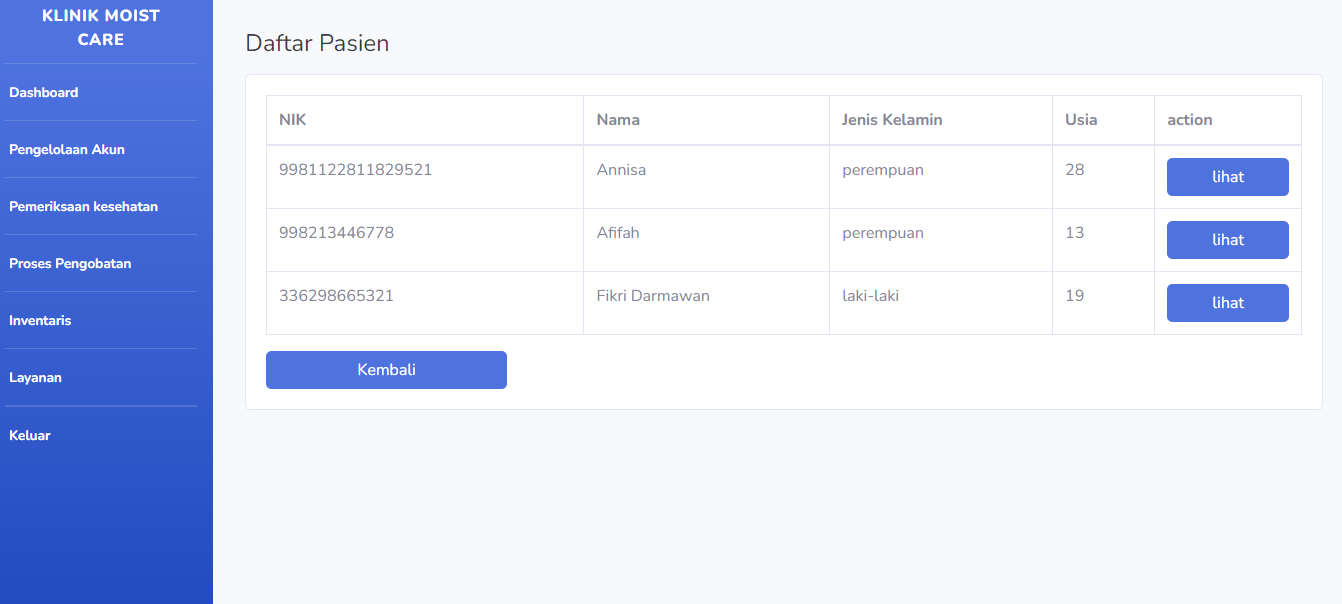
\includegraphics[width=14cm]{gambar/daftar_pasien_view.png}
		\caption{Realisasi \emph{view list} pasien terdaftar klinik} 
		\label{Gambar:usecaseadminjurnalpertama}
	\end{figure}

	\textbf{Gambar 4.33} merupakan \emph{view list} pasien terdaftar klinik. \emph{Code}-nya ada pada lampiran O.
	
	\item Implementasi \emph{web service list} pasien terdaftar klinik
	
	URL \emph{Routing} yang digunakan untuk \emph{list} pasien untuk terdaftar/terverifikasi klinik adalah jft.web.id/woundapiv2/list\_patient.
	
	\emph{Code} untuk \emph{web service} \emph{list} pasien untuk terdaftar/terverifikasi klinik ada pada lampiran P, metode yang digunakan adalah \emph{GET}. Pada saat pemanggilan \emph{web service} data berupa nama, jenis kelamin, usia dan NIK akan dipanggil untuk ditampilkan di tabel data \emph{list} pasien untuk terdaftar/terverifikasi klinik.
	
\end{enumerate}


\subsection{\emph{Sprint}-3}
\begin{table}[H]
	\centering
	\caption{\emph{Sprint}-3 \emph{backlog}}
	\label{tabel_input}
	\begin{tabular}{|c|l|l|l|}
		\hline
		\textbf{No} & \textbf{\emph{User Story}} & \textbf{\emph{Task}} &
		\textbf{Status}\\
		\hline
		
		1 & 
		Pemeriksaan & 
		1. implementasi \emph{view} hasil pemeriksaan &
		selesai\\
		
		& 
		kesehatan & 
		kesehatan.&
		\\
		
		& 
		& 
		2. implementasi \emph{web service} hasil&
		\\
		
		& 
		& 
		pemeriksaan kesehatan.&
		\\
		\hline
		
		2 & 
		Proses & 
		1. implementasi \emph{view} inventaris.&
		selesai\\
		
		& 
		pengobatan& 
		2. implementasi \emph{web service} inventaris.&
		\\
		
		& 
		& 
		3. implementasi \emph{view} layanan.
		&\\
		
		& 
		& 
		4. implementasi \emph{web service} layanan.&
		\\
		
		& 
		& 
		5. implementasi \emph{view} hasil pengkajian&
		tidak\\
		
		& 
		& 
		luka.&
		selesai\\
		
		
		& 
		& 
		6. implementasi \emph{web service} hasil&
		\\
		
		& 
		& 
		pengkajian luka.&
		\\
		
		& 
		& 
		7. implementasi \emph{view database} foto&
		\\
		
		& 
		& 
		luka yang dikategorisasikan per perawat.&
		\\
		
		& 
		& 
		8. implementasi \emph{web service database} foto&
		\\
		
		& 
		& 
		luka yang dikategorisasikan per perawat.&
		\\
		\hline
		
		3 & 
		Pendaftaran & 
		1. implementasi \emph{view} pendaftaran&
		tidak\\
		
		& 
		Pasien& 
		berobat.&
		selesai\\
		
		& 
		Berobat& 
		2. implementasi \emph{web service} pendaftaran&\\
		
		& 
		& 
		berobat.&\\
		\hline

	\end{tabular}
\end{table}

\begin{enumerate}
	\item Implementasi \emph{view} hasil pemeriksaan kesehatan
	
	Berikut merupakan implementasi \emph{view} detail hasil pemeriksaan kesehatan pasien sesuai tanggal yang admin pilih. \emph{Code}-nya ada pada lampiran Q dan menghasilkan tampilan \emph{view} seperti pada \textbf{Gambar 4.34}.
	
	\begin{figure}[H]
		\centering
		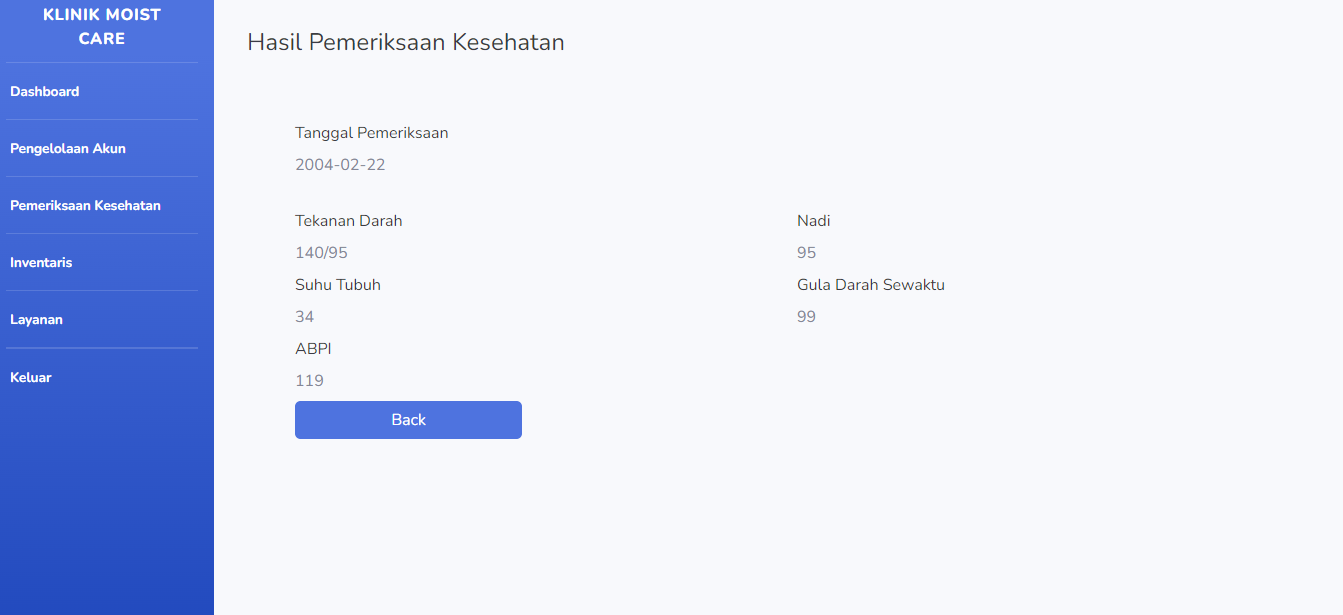
\includegraphics[width=14cm]{gambar/detail_hasil_pemeriksaan_kesehatan_view.png}
		\caption{Realisasi \emph{view} detail hasil pemeriksaan kesehatan seorang pasien berdasarkan tanggal pemeriksaan} 
		\label{Gambar:usecaseadminjurnalpertama}
	\end{figure}
	
	\item Implementasi \emph{web service} hasil pemeriksaan kesehatan
	
	URL \emph{Routing} yang digunakan untuk melakukan tambah hasil pemeriksaan kesehatan adalah jft.web.id/woundapiv2/add\_data\_pemeriksaan\_kesehatan.
	
	\emph{Code} untuk \emph{web service} tambah hasil pemeriksaan kesehatan ada pada lampiran R, metode yang digunakan adalah \emph{POST}. Pada saat pemanggilan \emph{web service}, perawat terlebih dulu mengisi tanggal, \emph{username} atau NIP, NIK pasien, tekanan darah, nadi, suhu, gula darah sewaktu, dan ABPI lalu akan dikembalikan ke pesan berhasil input data pemeriksaan kesehatan dengan status HTTP 200, jika data tidak sesuai maka akan dikembalikan ke pesan gagal input data pemeriksaan kesehatan dengan status HTTP 500.

	Dan \emph{code web service} untuk mendapatkan detail data hasil pemeriksaan kesehatan pasien berdasar tanggal pemeriksaan, yang kemudian akan ditampilkan pada \emph{view} detail hasil pemeriksaan kesehatan pasien. \emph{Code}-nya ada pada lampiran S.
	
	\item Implementasi \emph{view} inventaris
	
	Berikut merupakan implementasi \emph{view list} inventaris klinik. \emph{Code}-nya ada pada lampiran T dan menghasilkan tampilan \emph{view} seperti pada \textbf{Gambar 4.35}.
	
	\begin{figure}[H]
		\centering
		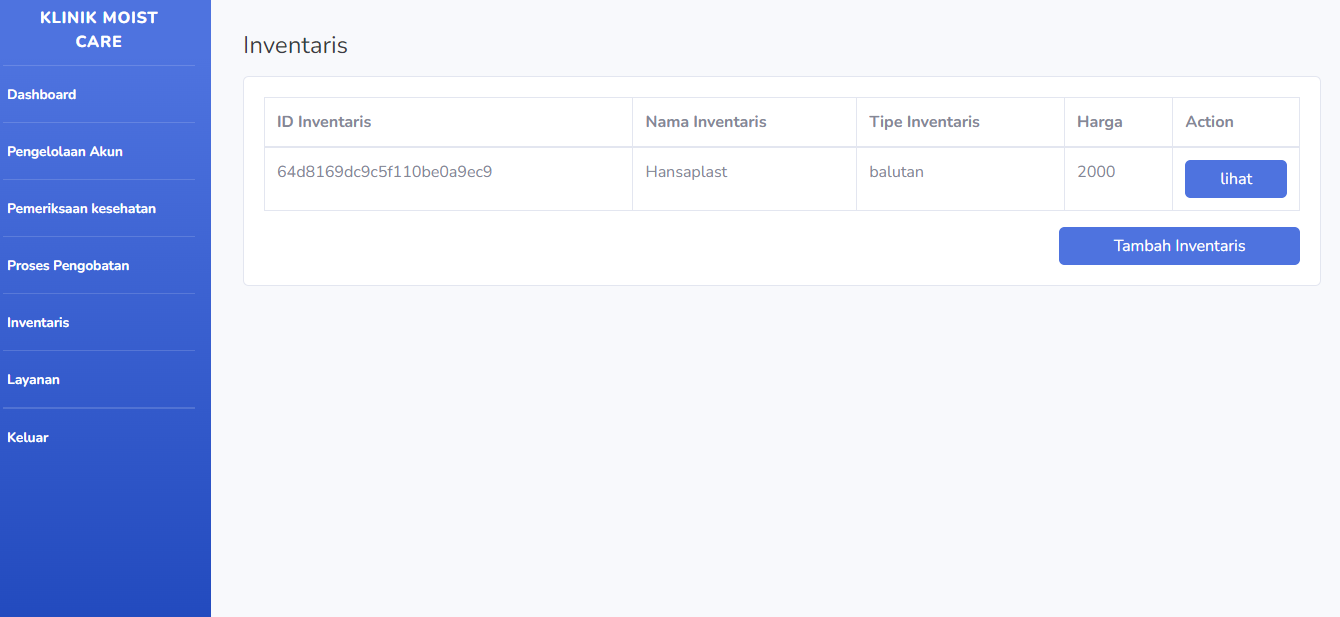
\includegraphics[width=14cm]{gambar/inventaris_view.png}
		\caption{Realisasi \emph{view} semua inventaris klinik} 
		\label{Gambar:usecaseadminjurnalpertama}
	\end{figure}
	
	\begin{figure}[H]
		\centering
		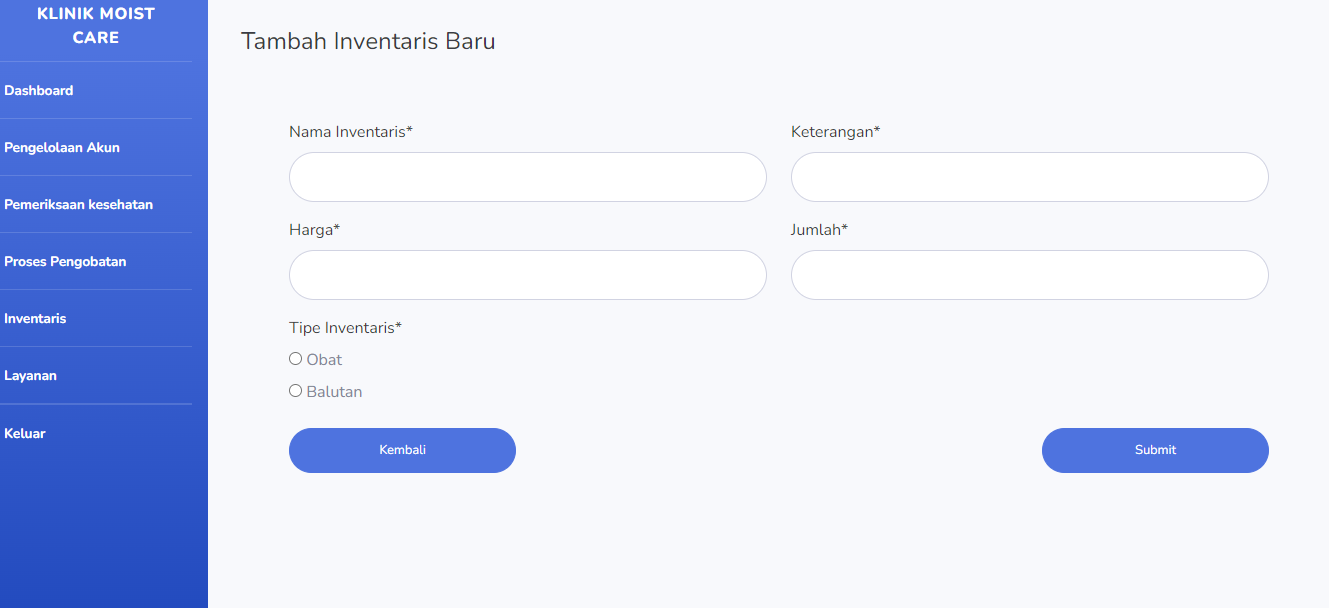
\includegraphics[width=14cm]{gambar/tambah_inventaris_view.png}
		\caption{Realisasi \emph{view} tambah inventaris klinik} 
		\label{Gambar:usecaseadminjurnalpertama}
	\end{figure}
	
	Jika admin menekan tombol aksi tambah inventaris maka akan diarahkan ke \emph{view} tambah inventaris. \emph{Code} -nya ada pada lampiran U dan menghasilkan tampilan \emph{view} seperti pada \textbf{Gambar 4.36}.
	
	\item Implementasi \emph{web service} inventaris
	
	URL \emph{Routing} yang digunakan untuk inventaris klinik adalah jft.web.id/woundapiv2/add\_inventaris.
	
	\emph{Code} untuk \emph{web service} tambah inventaris ada pada lampiran V, metode yang digunakan adalah \emph{POST}. admin akan diminta untuk mengisi data yang dibutuhkan untuk menambah inventaris, akan menampilkan pesan "berhasil input inventaris", dan menambah 1 inventaris ke dalam \emph{database} klinik. Jika gagal akan menampilkan pesan "gagal input inventaris".
	
	\item Implementasi \emph{view} layanan
	
	Berikut merupakan implementasi \emph{view list} layanan klinik. \emph{Code}-nya ada pada lampiran W dan menghasilkan tampilan \emph{view} seperti pada \textbf{Gambar 4.37}.
	
	\begin{figure}[H]
		\centering
		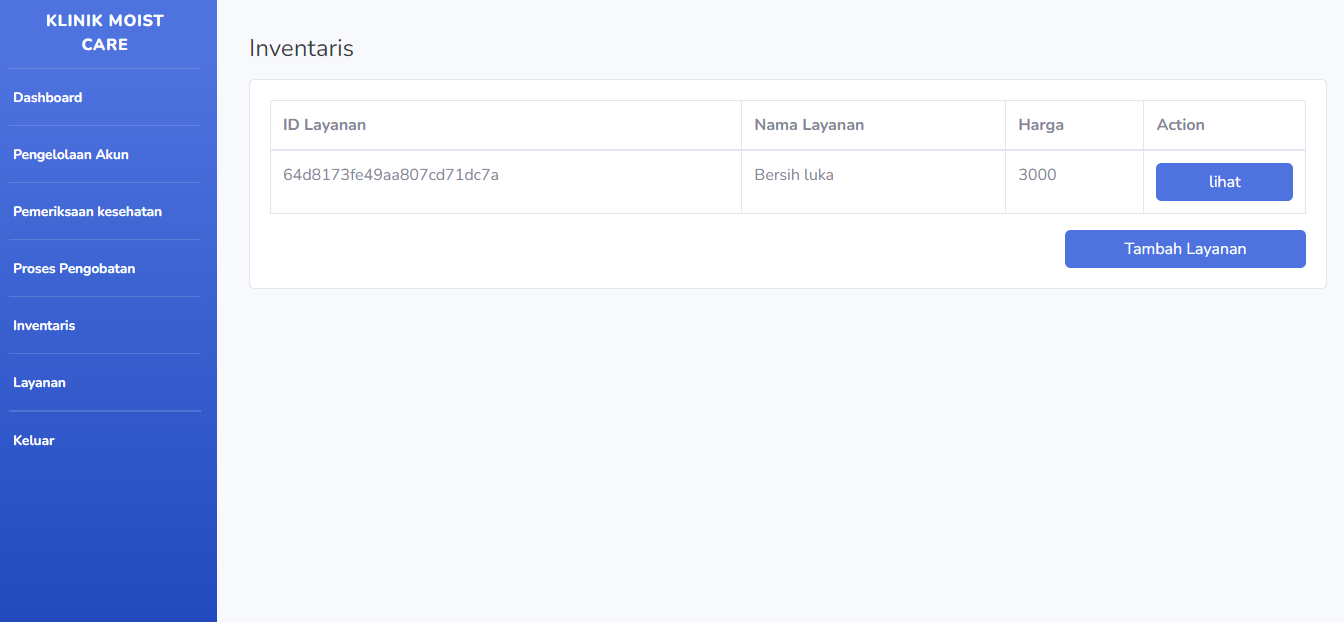
\includegraphics[width=14cm]{gambar/layanan_view.png}
		\caption{Realisasi \emph{view} semua layanan klinik} 
		\label{Gambar:usecaseadminjurnalpertama}
	\end{figure}
	
	Jika admin menekan tombol aksi tambah layanan maka akan diarahkan ke \emph{view} tambah layanan. Berikut merupakan \emph{code} ada pada lampiran X dan menghasilkan tampilan \emph{view} seperti pada \textbf{Gambar 4.38}.
	
	\begin{figure}[H]
		\centering
		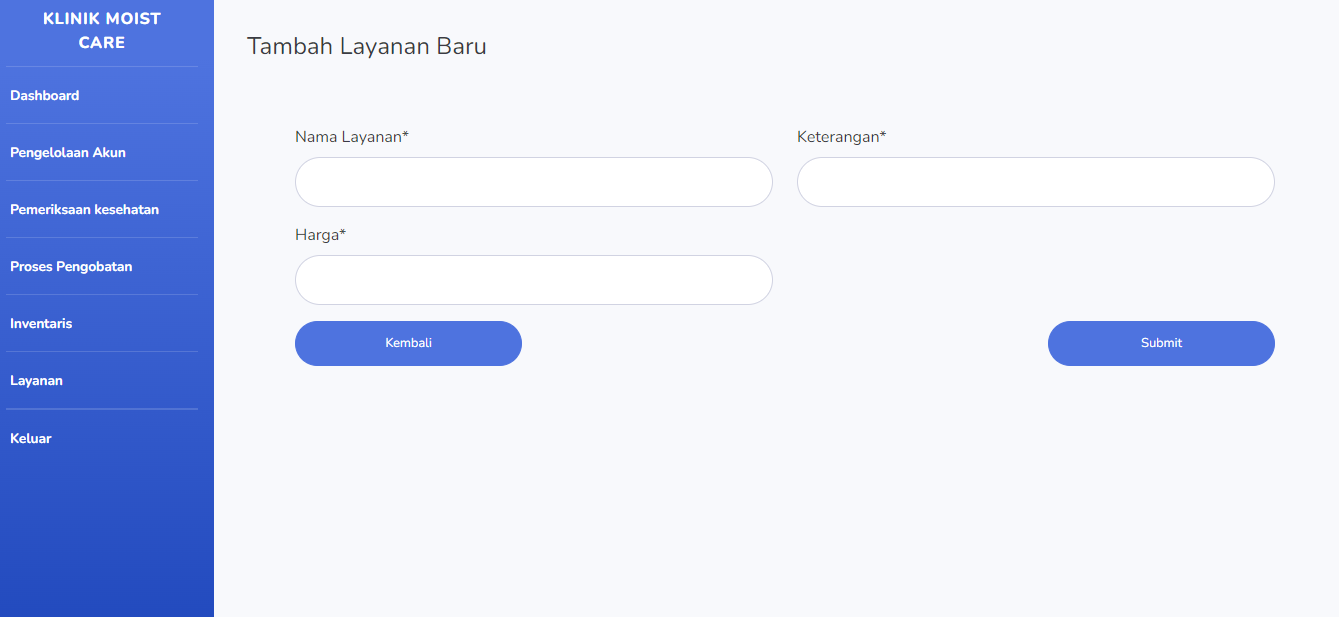
\includegraphics[width=14cm]{gambar/tambah_layanan_view.png}
		\caption{Realisasi \emph{view} tambah layanan klinik} 
		\label{Gambar:usecaseadminjurnalpertama}
	\end{figure}
	
	\item Implementasi \emph{web service} layanan
	
	URL \emph{Routing} yang digunakan untuk layanan klinik adalah jft.web.id/woundapiv2/add\_layanan.
	
	\emph{Code} untuk \emph{web service} tambah layanan klinik ada pada lampiran Y, metode yang digunakan adalah \emph{POST}. admin akan diminta untuk mengisi data yang dibutuhkan untuk menambah layanan, menampilkan pesan "berhasil input layanan", dan menambah 1 layanan ke dalam \emph{database} klinik. Jika gagal akan menampilkan pesan "gagal input layanan".
	
	%\item Implementasi \emph{view} hasil pengkajian luka
	
	%Status dari \emph{task} ini adalah tidak terselesaikan
	
	%\item Implementasi \emph{web service} hasil hasil pengkajian luka
	
	%Status dari \emph{task} ini adalah tidak terselesaikan
	
	%\item Implementasi \emph{view database} foto luka yang dikategorisasikan per perawat
	
	%Status dari \emph{task} ini adalah tidak terselesaikan
	
	%\item Implementasi \emph{web service database} foto luka yang dikategorisasikan per perawat
	
	%Status dari \emph{task} ini adalah tidak terselesaikan
	
	%\item Implementasi \emph{view} pendaftaran berobat
	
	%Status dari \emph{task} ini adalah tidak terselesaikan
	
	%\item Implementasi \emph{web service} pendaftaran berobat
	
	%Status dari \emph{task} ini adalah tidak terselesaikan
	
\end{enumerate}

\subsection{\emph{Sprint}-4}

\emph{Sprint}-4 tidak terencanakan.

\subsection{Laporan akhir pengembangan sistem}
Pada Penelitian ini, fitur pada sistem yang selesai peneliti buat adalah:

\begin{enumerate}
	\item pembuatan akun pasien
	\item \emph{dashboard} klinik
	\item pemeriksaan kesehatan
	\item sebagian proses pengobatan luka (\emph{view} dan \emph{web service} inventaris dan layanan)
\end{enumerate}

Dan fitur pada sistem yang tidak selesai peneliti buat adalah:

\begin{enumerate}
	\item proses pengobatan luka
	\item pendaftaran pasien berobat
	\item pengelolaan antrian
	\item administrasi keuangan
	\item sebagian proses pengobatan luka (\emph{view} dan \emph{web service} hasil pengkajian luka dan \emph{database} foto luka yang dikategorisasikan berdasarkan perawat)
\end{enumerate}

Peneliti tidak dapat menuntaskan pengembangan sistem informasi keperawatan luka karena beberapa hal, yaitu:

\begin{enumerate}
	\item \emph{Lack of skill}
	
	Pada saat pengembangan sistem berlangsung, peneliti juga mempelajari teknologi-teknologi yang diperlukan untuk pengembangan sistem karena peneliti tidak menguasai teknologi yang akan dipakai. Sehingga peneliti membutuhkan waktu yang lebih lama untuk pengembangannya, dimana deskripsi ini berkaitan dengan poin selanjutnya.
	
	\item Waktu yang diberikan untuk merancang sistem yang kurang
	
	Seperti yang sudah dijelaskan pada poin sebelumnya, dikarenakan peneliti membutuhkan waktu yang lebih lama untuk pengembangannya karena  disamping mengembangkan, peneliti juga harus belajar kembali teknologi yang belum dikuasai. sehingga waktu yang direncanakan dalam mengerjakan sistem dirasa sangat kurang untuk peneliti bisa menyelesaikan sistem yang ingin dibuat.
	
\end{enumerate}

% Baris ini digunakan untuk membantu dalam melakukan sitasi
% Karena diapit dengan comment, maka baris ini akan diabaikan
% oleh compiler LaTeX.
\begin{comment}
\bibliography{daftar-pustaka}
\end{comment}